\documentclass[]{book}
\usepackage{lmodern}
\usepackage{amssymb,amsmath}
\usepackage{ifxetex,ifluatex}
\usepackage{fixltx2e} % provides \textsubscript
\ifnum 0\ifxetex 1\fi\ifluatex 1\fi=0 % if pdftex
  \usepackage[T1]{fontenc}
  \usepackage[utf8]{inputenc}
\else % if luatex or xelatex
  \ifxetex
    \usepackage{mathspec}
  \else
    \usepackage{fontspec}
  \fi
  \defaultfontfeatures{Ligatures=TeX,Scale=MatchLowercase}
\fi
% use upquote if available, for straight quotes in verbatim environments
\IfFileExists{upquote.sty}{\usepackage{upquote}}{}
% use microtype if available
\IfFileExists{microtype.sty}{%
\usepackage{microtype}
\UseMicrotypeSet[protrusion]{basicmath} % disable protrusion for tt fonts
}{}
\usepackage[margin=1in]{geometry}
\usepackage{hyperref}
\hypersetup{unicode=true,
            pdftitle={YaRrr! The Pirate's Guide to R},
            pdfauthor={Nathaniel D. Phillips},
            pdfborder={0 0 0},
            breaklinks=true}
\urlstyle{same}  % don't use monospace font for urls
\usepackage{natbib}
\bibliographystyle{apalike}
\usepackage{color}
\usepackage{fancyvrb}
\newcommand{\VerbBar}{|}
\newcommand{\VERB}{\Verb[commandchars=\\\{\}]}
\DefineVerbatimEnvironment{Highlighting}{Verbatim}{commandchars=\\\{\}}
% Add ',fontsize=\small' for more characters per line
\usepackage{framed}
\definecolor{shadecolor}{RGB}{248,248,248}
\newenvironment{Shaded}{\begin{snugshade}}{\end{snugshade}}
\newcommand{\KeywordTok}[1]{\textcolor[rgb]{0.13,0.29,0.53}{\textbf{{#1}}}}
\newcommand{\DataTypeTok}[1]{\textcolor[rgb]{0.13,0.29,0.53}{{#1}}}
\newcommand{\DecValTok}[1]{\textcolor[rgb]{0.00,0.00,0.81}{{#1}}}
\newcommand{\BaseNTok}[1]{\textcolor[rgb]{0.00,0.00,0.81}{{#1}}}
\newcommand{\FloatTok}[1]{\textcolor[rgb]{0.00,0.00,0.81}{{#1}}}
\newcommand{\ConstantTok}[1]{\textcolor[rgb]{0.00,0.00,0.00}{{#1}}}
\newcommand{\CharTok}[1]{\textcolor[rgb]{0.31,0.60,0.02}{{#1}}}
\newcommand{\SpecialCharTok}[1]{\textcolor[rgb]{0.00,0.00,0.00}{{#1}}}
\newcommand{\StringTok}[1]{\textcolor[rgb]{0.31,0.60,0.02}{{#1}}}
\newcommand{\VerbatimStringTok}[1]{\textcolor[rgb]{0.31,0.60,0.02}{{#1}}}
\newcommand{\SpecialStringTok}[1]{\textcolor[rgb]{0.31,0.60,0.02}{{#1}}}
\newcommand{\ImportTok}[1]{{#1}}
\newcommand{\CommentTok}[1]{\textcolor[rgb]{0.56,0.35,0.01}{\textit{{#1}}}}
\newcommand{\DocumentationTok}[1]{\textcolor[rgb]{0.56,0.35,0.01}{\textbf{\textit{{#1}}}}}
\newcommand{\AnnotationTok}[1]{\textcolor[rgb]{0.56,0.35,0.01}{\textbf{\textit{{#1}}}}}
\newcommand{\CommentVarTok}[1]{\textcolor[rgb]{0.56,0.35,0.01}{\textbf{\textit{{#1}}}}}
\newcommand{\OtherTok}[1]{\textcolor[rgb]{0.56,0.35,0.01}{{#1}}}
\newcommand{\FunctionTok}[1]{\textcolor[rgb]{0.00,0.00,0.00}{{#1}}}
\newcommand{\VariableTok}[1]{\textcolor[rgb]{0.00,0.00,0.00}{{#1}}}
\newcommand{\ControlFlowTok}[1]{\textcolor[rgb]{0.13,0.29,0.53}{\textbf{{#1}}}}
\newcommand{\OperatorTok}[1]{\textcolor[rgb]{0.81,0.36,0.00}{\textbf{{#1}}}}
\newcommand{\BuiltInTok}[1]{{#1}}
\newcommand{\ExtensionTok}[1]{{#1}}
\newcommand{\PreprocessorTok}[1]{\textcolor[rgb]{0.56,0.35,0.01}{\textit{{#1}}}}
\newcommand{\AttributeTok}[1]{\textcolor[rgb]{0.77,0.63,0.00}{{#1}}}
\newcommand{\RegionMarkerTok}[1]{{#1}}
\newcommand{\InformationTok}[1]{\textcolor[rgb]{0.56,0.35,0.01}{\textbf{\textit{{#1}}}}}
\newcommand{\WarningTok}[1]{\textcolor[rgb]{0.56,0.35,0.01}{\textbf{\textit{{#1}}}}}
\newcommand{\AlertTok}[1]{\textcolor[rgb]{0.94,0.16,0.16}{{#1}}}
\newcommand{\ErrorTok}[1]{\textcolor[rgb]{0.64,0.00,0.00}{\textbf{{#1}}}}
\newcommand{\NormalTok}[1]{{#1}}
\usepackage{longtable,booktabs}
\usepackage{graphicx,grffile}
\makeatletter
\def\maxwidth{\ifdim\Gin@nat@width>\linewidth\linewidth\else\Gin@nat@width\fi}
\def\maxheight{\ifdim\Gin@nat@height>\textheight\textheight\else\Gin@nat@height\fi}
\makeatother
% Scale images if necessary, so that they will not overflow the page
% margins by default, and it is still possible to overwrite the defaults
% using explicit options in \includegraphics[width, height, ...]{}
\setkeys{Gin}{width=\maxwidth,height=\maxheight,keepaspectratio}
\IfFileExists{parskip.sty}{%
\usepackage{parskip}
}{% else
\setlength{\parindent}{0pt}
\setlength{\parskip}{6pt plus 2pt minus 1pt}
}
\setlength{\emergencystretch}{3em}  % prevent overfull lines
\providecommand{\tightlist}{%
  \setlength{\itemsep}{0pt}\setlength{\parskip}{0pt}}
\setcounter{secnumdepth}{5}
% Redefines (sub)paragraphs to behave more like sections
\ifx\paragraph\undefined\else
\let\oldparagraph\paragraph
\renewcommand{\paragraph}[1]{\oldparagraph{#1}\mbox{}}
\fi
\ifx\subparagraph\undefined\else
\let\oldsubparagraph\subparagraph
\renewcommand{\subparagraph}[1]{\oldsubparagraph{#1}\mbox{}}
\fi

%%% Use protect on footnotes to avoid problems with footnotes in titles
\let\rmarkdownfootnote\footnote%
\def\footnote{\protect\rmarkdownfootnote}

%%% Change title format to be more compact
\usepackage{titling}

% Create subtitle command for use in maketitle
\newcommand{\subtitle}[1]{
  \posttitle{
    \begin{center}\large#1\end{center}
    }
}

\setlength{\droptitle}{-2em}
  \title{YaRrr! The Pirate's Guide to R}
  \pretitle{\vspace{\droptitle}\centering\huge}
  \posttitle{\par}
  \author{Nathaniel D. Phillips}
  \preauthor{\centering\large\emph}
  \postauthor{\par}
  \predate{\centering\large\emph}
  \postdate{\par}
  \date{2017-02-21}

\usepackage{booktabs}
\usepackage{amsthm}
\makeatletter
\def\thm@space@setup{%
  \thm@preskip=8pt plus 2pt minus 4pt
  \thm@postskip=\thm@preskip
}
\makeatother

\usepackage{amsthm}
\newtheorem{theorem}{Theorem}[chapter]
\newtheorem{lemma}{Lemma}[chapter]
\theoremstyle{definition}
\newtheorem{definition}{Definition}[chapter]
\newtheorem{corollary}{Corollary}[chapter]
\newtheorem{proposition}{Proposition}[chapter]
\theoremstyle{definition}
\newtheorem{example}{Example}[chapter]
\theoremstyle{remark}
\newtheorem*{remark}{Remark}
\begin{document}
\maketitle

{
\setcounter{tocdepth}{1}
\tableofcontents
}
\chapter{Preface}\label{intro}

\begin{center}
\includegraphics[width=600px]{images/YaRrr_Cover} \end{center}

The purpose of this book is to help you learn R from the ground-up.

\section{Where did this book come
from?}\label{where-did-this-book-come-from}

Let me make something very, very clear\ldots{}

\emph{I did not write this book}.

This whole story started in the Summer of 2015. I was taking a late
night swim on the Bodensee in Konstanz and saw a rusty object sticking
out of the water. Upon digging it out, I realized it was an ancient
usb-stick with the word YaRrr inscribed on the side. Intrigued, I
brought it home and plugged it into my laptop. Inside the stick, I found
a single pdf file written entirely in pirate-speak. After watching
several pirate movies, I learned enough pirate-speak to begin
translating the text to English. Sure enough, the book turned out to be
an introduction to R called The Pirate's Guide to R.

This book clearly has both massive historical and pedagogical
significance. Most importantly, it turns out that pirates were
programming in R well before the earliest known advent of computers. Of
slightly less significance is that the book has turned out to be a
surprisingly up-to-date and approachable introductory text to R. For
both of these reasons, I felt it was my duty to share the book with the
world.

If you or spot any typos or errors, or have any recommendations for
future versions of the book, please write me at YaRrr.Book@gmail.com or
tweet me @YaRrrBook.

\section{Who is this book for?}\label{who-is-this-book-for}

While this book was originally written for pirates, I think that anyone
who wants to learn R can benefit from this book. If you haven't had an
introductory course in statistics, some of the later statistical
concepts may be difficult, but I'll try my best to add brief
descriptions of new topics when necessary. Likewise, if R is your first
programming language, you'll likely find the first few chapters quite
challenging as you learn the basics of programming. However, if R is
your first programming language, that's totally fine as what you learn
here will help you in learning other languages as well (if you choose
to). Finally, while the techniques in this book apply to most data
analysis problems, because my background is in experimental psychology I
will cater the course to solving analysis problems commonly faced in
psychological research.

\textbf{What this book is}

This book is meant to introduce you to the basic analytical tools in R,
from basic coding and analyses, to data wrangling, plotting, and
statistical inference.

\textbf{What this book is not}

This book does not cover any one topic in extensive detail. If you are
interested in conducting analyses or creating plots not covered in the
book, I'm sure you'll find the answer with a quick Google search!

\section{Why is R so great?}\label{why-is-r-so-great}

As you've already gotten this book, you probably already have some idea
why R is so great. However, in order to help prevent you from giving up
the first time you run into a programming wall, let me give you a few
more reasons:

\begin{enumerate}
\def\labelenumi{\arabic{enumi}.}
\item
  R is 100\% free and as a result, has a huge support community. Unlike
  SPSS, Matlab, Excel and JMP, R is, and always will be completely free.
  This doesn't just help your wallet - it means that a huge community of
  R programmers will constantly develop an distribute new R
  functionality and packages at a speed that leaves all those other
  packages in the dust! Unlike Fight Club, the first rule of R is ``Do
  talk about R!'' The size of the R programming community is staggering.
  If you ever have a question about how to implement something in R, a
  quick
  Poogle\footnote{I am in the process of creating Poogle - Google for Pirates. Kickstarter page coming soon...}
  search will lead you to your answer virtually every single time.
\item
  R is the presnt, and future of statistical programming. To illustrate
  this, look at the following three figures. These are Google trend
  searches for three terms: R Programming, Matlab, and SPSS. Try and
  guess which one is which.
\end{enumerate}

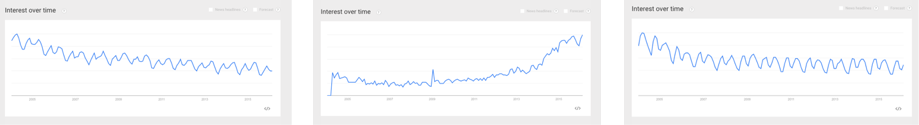
\includegraphics{images/googletrends.png}

\begin{enumerate}
\def\labelenumi{\arabic{enumi}.}
\setcounter{enumi}{2}
\item
  R is incredibly versatile. You can use R to do everything from
  calculating simple summary statistics, to performing complex
  simulations to creating gorgeous plots like the chord diagram on the
  right. If you can imagine an analytical task, you can almost certainly
  implement it in R.
\item
  Using RStudio, a program to help you write R code, You can easily and
  seamlessly combine R code, analyses, plots, and written text into
  elegant documents all in one place using Sweave (R and Latex) or
  RMarkdown. In fact, I translated this entire book (the text,
  formatting, plots, code\ldots{}yes, everything) in RStudio using
  Sweave. With RStudio and Sweave, instead of trying to manage two or
  three programs, say Excel, Word and (sigh) SPSS, where you find
  yourself spending half your time copying, pasting and formatting data,
  images and test, you can do everything in one place so nothing gets
  misread, mistyped, or forgotten.
\end{enumerate}

\begin{Shaded}
\begin{Highlighting}[]
\NormalTok{circlize::}\KeywordTok{chordDiagram}\NormalTok{(}\KeywordTok{matrix}\NormalTok{(}\KeywordTok{sample}\NormalTok{(}\DecValTok{10}\NormalTok{), }
                              \DataTypeTok{nrow =} \DecValTok{2}\NormalTok{, }\DataTypeTok{ncol =} \DecValTok{5}\NormalTok{))}
\end{Highlighting}
\end{Shaded}

\begin{figure}[htbp]
\centering
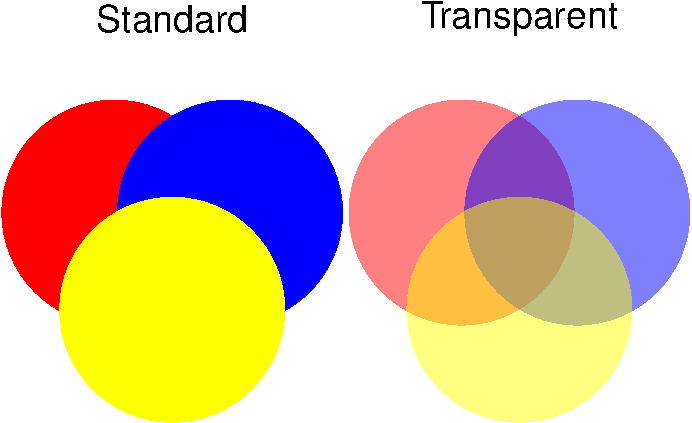
\includegraphics{YaRrr_files/figure-latex/unnamed-chunk-3-1.pdf}
\caption{\label{fig:unnamed-chunk-3}A super cool chord diagram from the
circlize package}
\end{figure}

\begin{enumerate}
\def\labelenumi{\arabic{enumi}.}
\setcounter{enumi}{4}
\item
  Analyses conducted in R are transparent, easily shareable, and
  reproducible. If you ask an SPSS user how they conducted a specific
  analyses, they will either A) Not remember, B) Try (nervously) to
  construct an analysis procedure on the spot that makes sense - which
  may or may not correspond to what they actually did months or years
  ago, or C) Ask you what you are doing in their house. I used to
  primarily use SPSS, so I speak from experience on this. If you ask an
  R user (who uses good programming techniques!) how they conducted an
  analysis, they should always be able to show you the exact code they
  used. Of course, this doesn't mean that they used the appropriate
  analysis or interpreted it correctly, but with all the original code,
  any problems should be completely transparent!
\item
  And most importantly of all, R is the programming language of choice
  for pirates.
\end{enumerate}

\section{R is like a
relationship\ldots{}}\label{r-is-like-a-relationship}

Yes, R is very much like a relationship. Like relationships, there are
two major truths to R programming:

\begin{figure}

{\centering 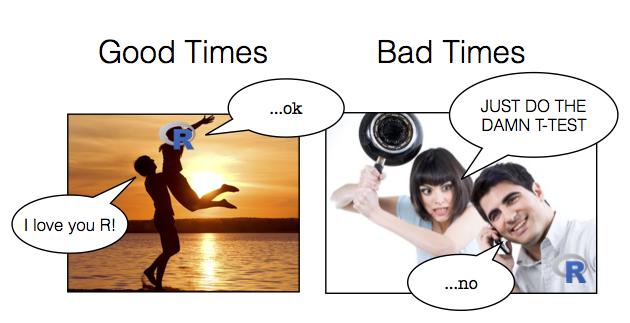
\includegraphics{images/rrelationship} 

}

\caption{Yep, R will become both your best friend and your worst nightmare. The bad times will make the good times oh so much sweeter.}\label{fig:unnamed-chunk-4}
\end{figure}

\begin{enumerate}
\def\labelenumi{\arabic{enumi}.}
\item
  There is nothing more \emph{frustrating} than when your code does
  \emph{not} work
\item
  There is nothing more \emph{satisfying} than when your code
  \emph{does} work!
\end{enumerate}

Anything worth doing, from losing weight to getting a degree, takes
time. Learning R is no different. Especially if this is your first
experience programming, you are going to experience a \emph{lot} of
headaches when you get started. You will run into error after error and
pound your fists against the table screaming: ``WHY ISN'T MY CODE
WORKING?!?!? There must be something wrong with this stupid
software!!!'' You will spend hours trying to find a bug in your code,
only to find that - frustratingly enough, you had had an extra space or
missed a comma somewhere. You'll then wonder why you ever decided to
learn R when (::sigh::) SPSS was so ``nice and easy.''

\begin{figure}

{\centering 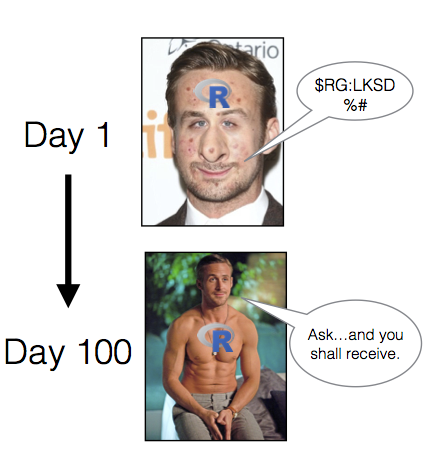
\includegraphics{images/gosling} 

}

\caption{When you first meet R, it will look so fugly that you'll wonder if this is all some kind of sick joke. But trust me, once you learn how to talk to it, and clean it up a bit, all your friends will be crazy jealous.}\label{fig:unnamed-chunk-5}
\end{figure}

\textbf{Fun Fact!} SPSS stands for ``Shitty Piece of Shitty Shit''. True
story.

This is perfectly normal! Don't get discouraged and DON'T GO BACK TO
SPSS! That would be quitting on exercise altogether because you had a
tough workout.

Trust me, as you gain more programming experience, you'll experience
fewer and fewer bugs (though they'll never go away completely). Once you
get over the initial barriers, you'll find yourself conducting analyses
much, much faster than you ever did before.

\section{Who am I?}\label{who-am-i}

\begin{figure}

{\centering 
\includegraphics[width=7.49in]{images/beer} 

}

\caption{Like a pirate, I work best with a mug of beer within arms' reach.}\label{fig:unnamed-chunk-6}
\end{figure}

My name is Nathaniel -- not Nathan\ldots{}not Nate\ldots{}and
\emph{definitely} not Nat. I am a psychologist with a background in
statistics and judgment and decision making. You can find my R (and
non-R) related musings at \url{http://ndphillips.github.io}

\chapter{Getting Started}\label{started}

\section{Installing (Base) R and
RStudio}\label{installing-base-r-and-rstudio}

First things first, let's download both Base R and Rstudio. Again, R is
the basic software which contains the R programming language. RStudio is
software that makes R programming easier. Of course, they are totally
free and open source.

\begin{figure}
\includegraphics[width=200px]{images/rlogo} \end{figure}

\begin{longtable}[]{@{}ll@{}}
\toprule
Operating System & Link\tabularnewline
\midrule
\endhead
Windows &
\url{http://cran.r-project.org/bin/windows/base/}\tabularnewline
Mac & \url{http://cran.r-project.org/bin/macosx/}\tabularnewline
\bottomrule
\end{longtable}

Once you've installed base R on your computer, try opening it. When you
do you should see a screen like the one in Figure \ref{fig:rscreenshot}
(this is the Mac version). As you can see, base R is very much
bare-bones software. It's kind of the equivalent of a simple text editor
that comes with your computer.

\textbackslash{}begin\{figure\}

\{\centering 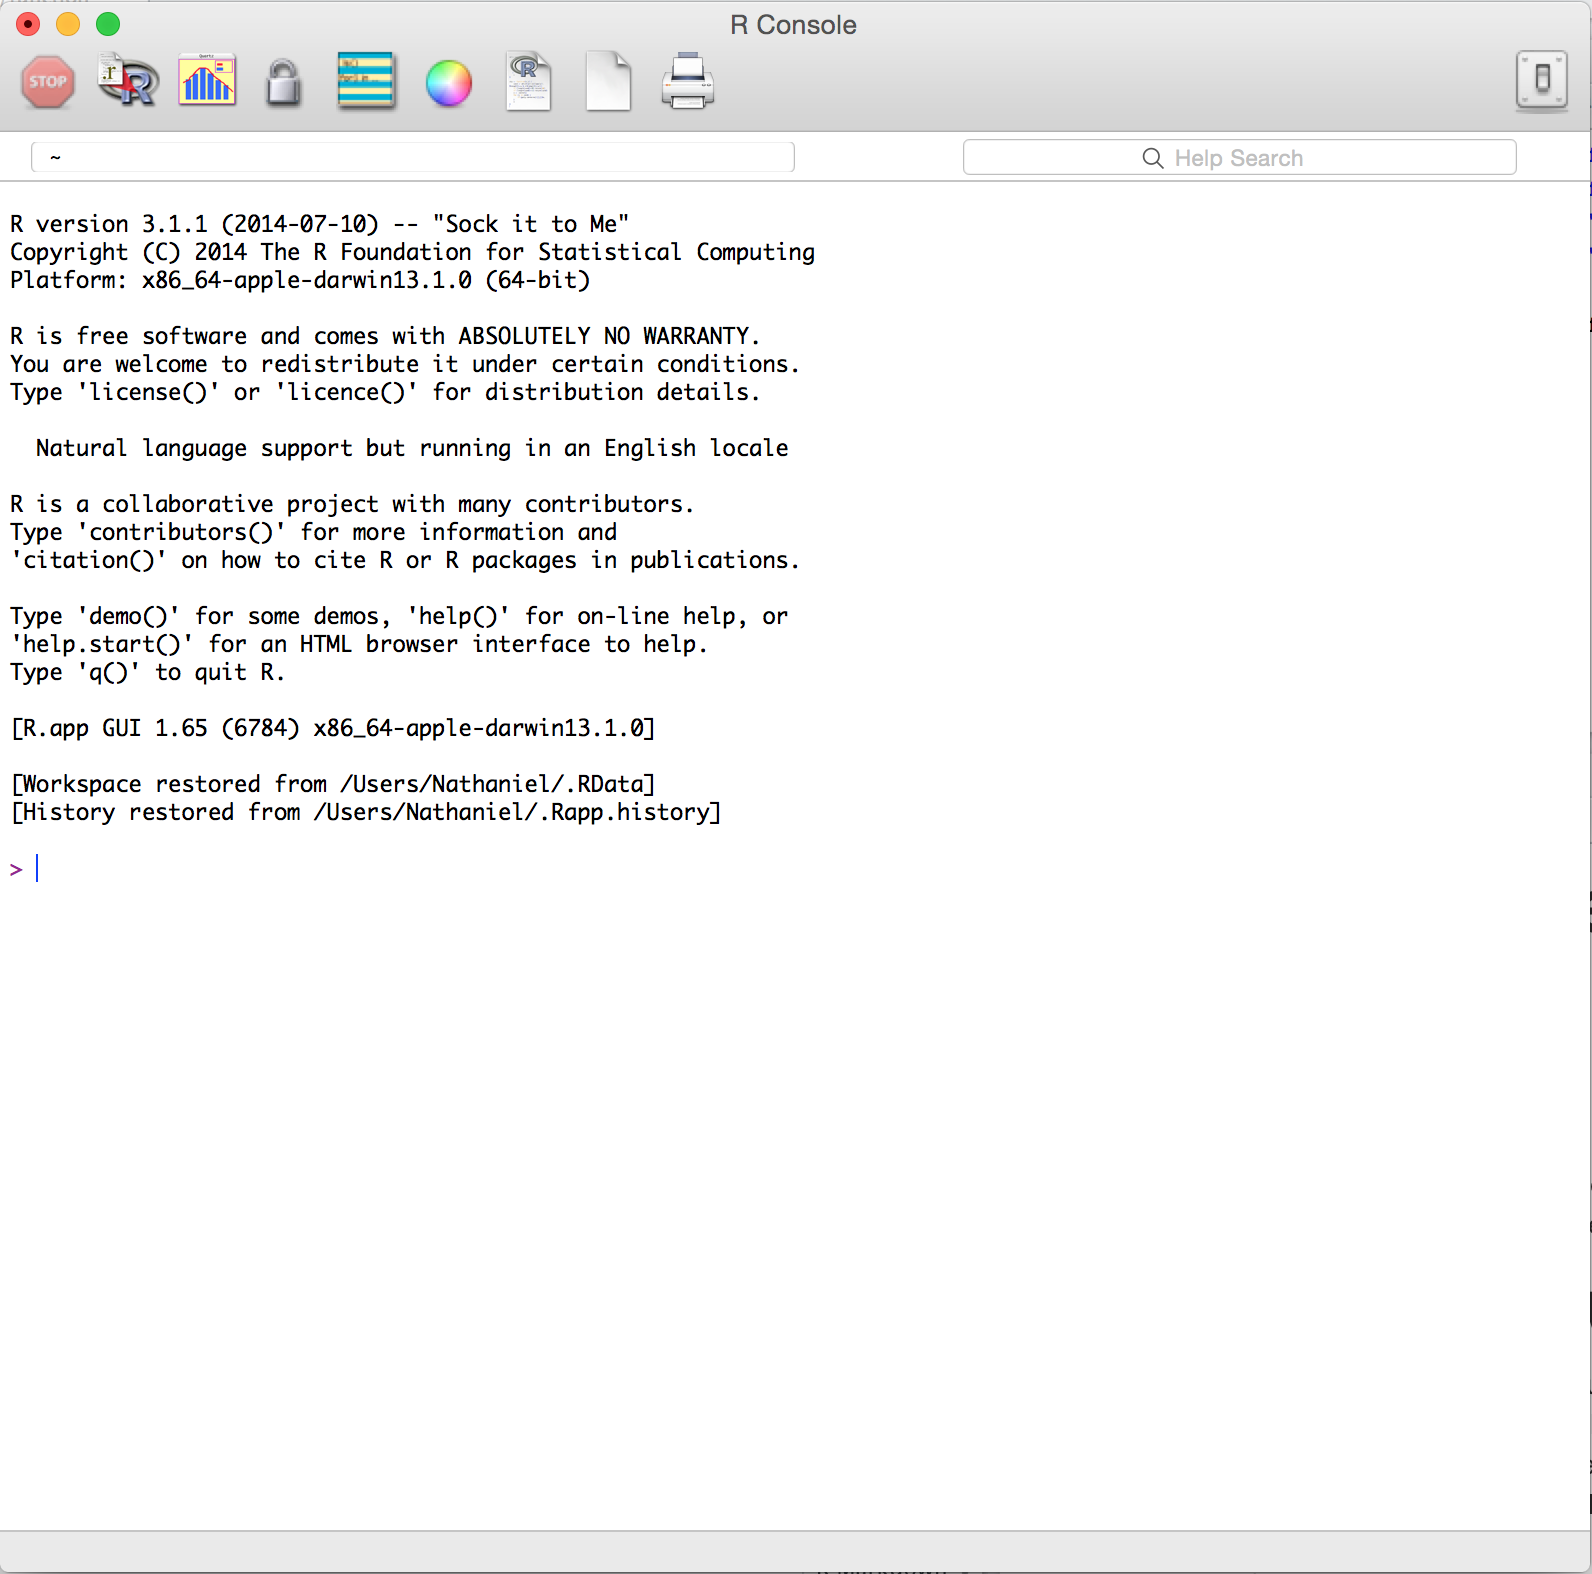
\includegraphics[width=400px]{images/RScreenshot}

\}

\textbackslash{}caption\{\{Here is how the base R application looks.
While you can use the base R application alone, most people I know use
RStudio -- software that helps you to write and use R code more
efficiently!\}\label{fig:unnamed-chunk-8} \textbackslash{}end\{figure\}

While you can do pretty much everything you want within base R, you'll
find that most people these days do their R programming in an
application called RStudio. RStudio is a graphical user interface
(GUI)-like interface for R that makes programming in R a bit easier. In
fact, once you've installed RStudio, you'll likely never need to open
the base R application again. To download and install RStudio (around
40mb), go to one of the links above and follow the instructions.

\begin{figure}

\includegraphics[width=200px]{images/RStudio} \end{figure}

\begin{longtable}[]{@{}ll@{}}
\toprule
Operating System & Link\tabularnewline
\midrule
\endhead
All &
\url{http://www.rstudio.com/products/rstudio/download/}\tabularnewline
\bottomrule
\end{longtable}

Let's go ahead and boot up RStudio and see how she looks!

\section{The four RStudio Windows}\label{the-four-rstudio-windows}

When you open RStudio, you'll see the following four windows (also
called panes) shown in in Figure \ref{fig:rstudiowindows}. However, your
windows might be in a different order that those in Figure
\ref{fig:rstudiowindows}. If you'd like, you can change the order of the
windows under RStudio preferences. You can also change their shape by
either clicking the minimize or maximize buttons on the top right of
each panel, or by clicking and dragging the middle of the borders of the
windows.

\begin{figure}
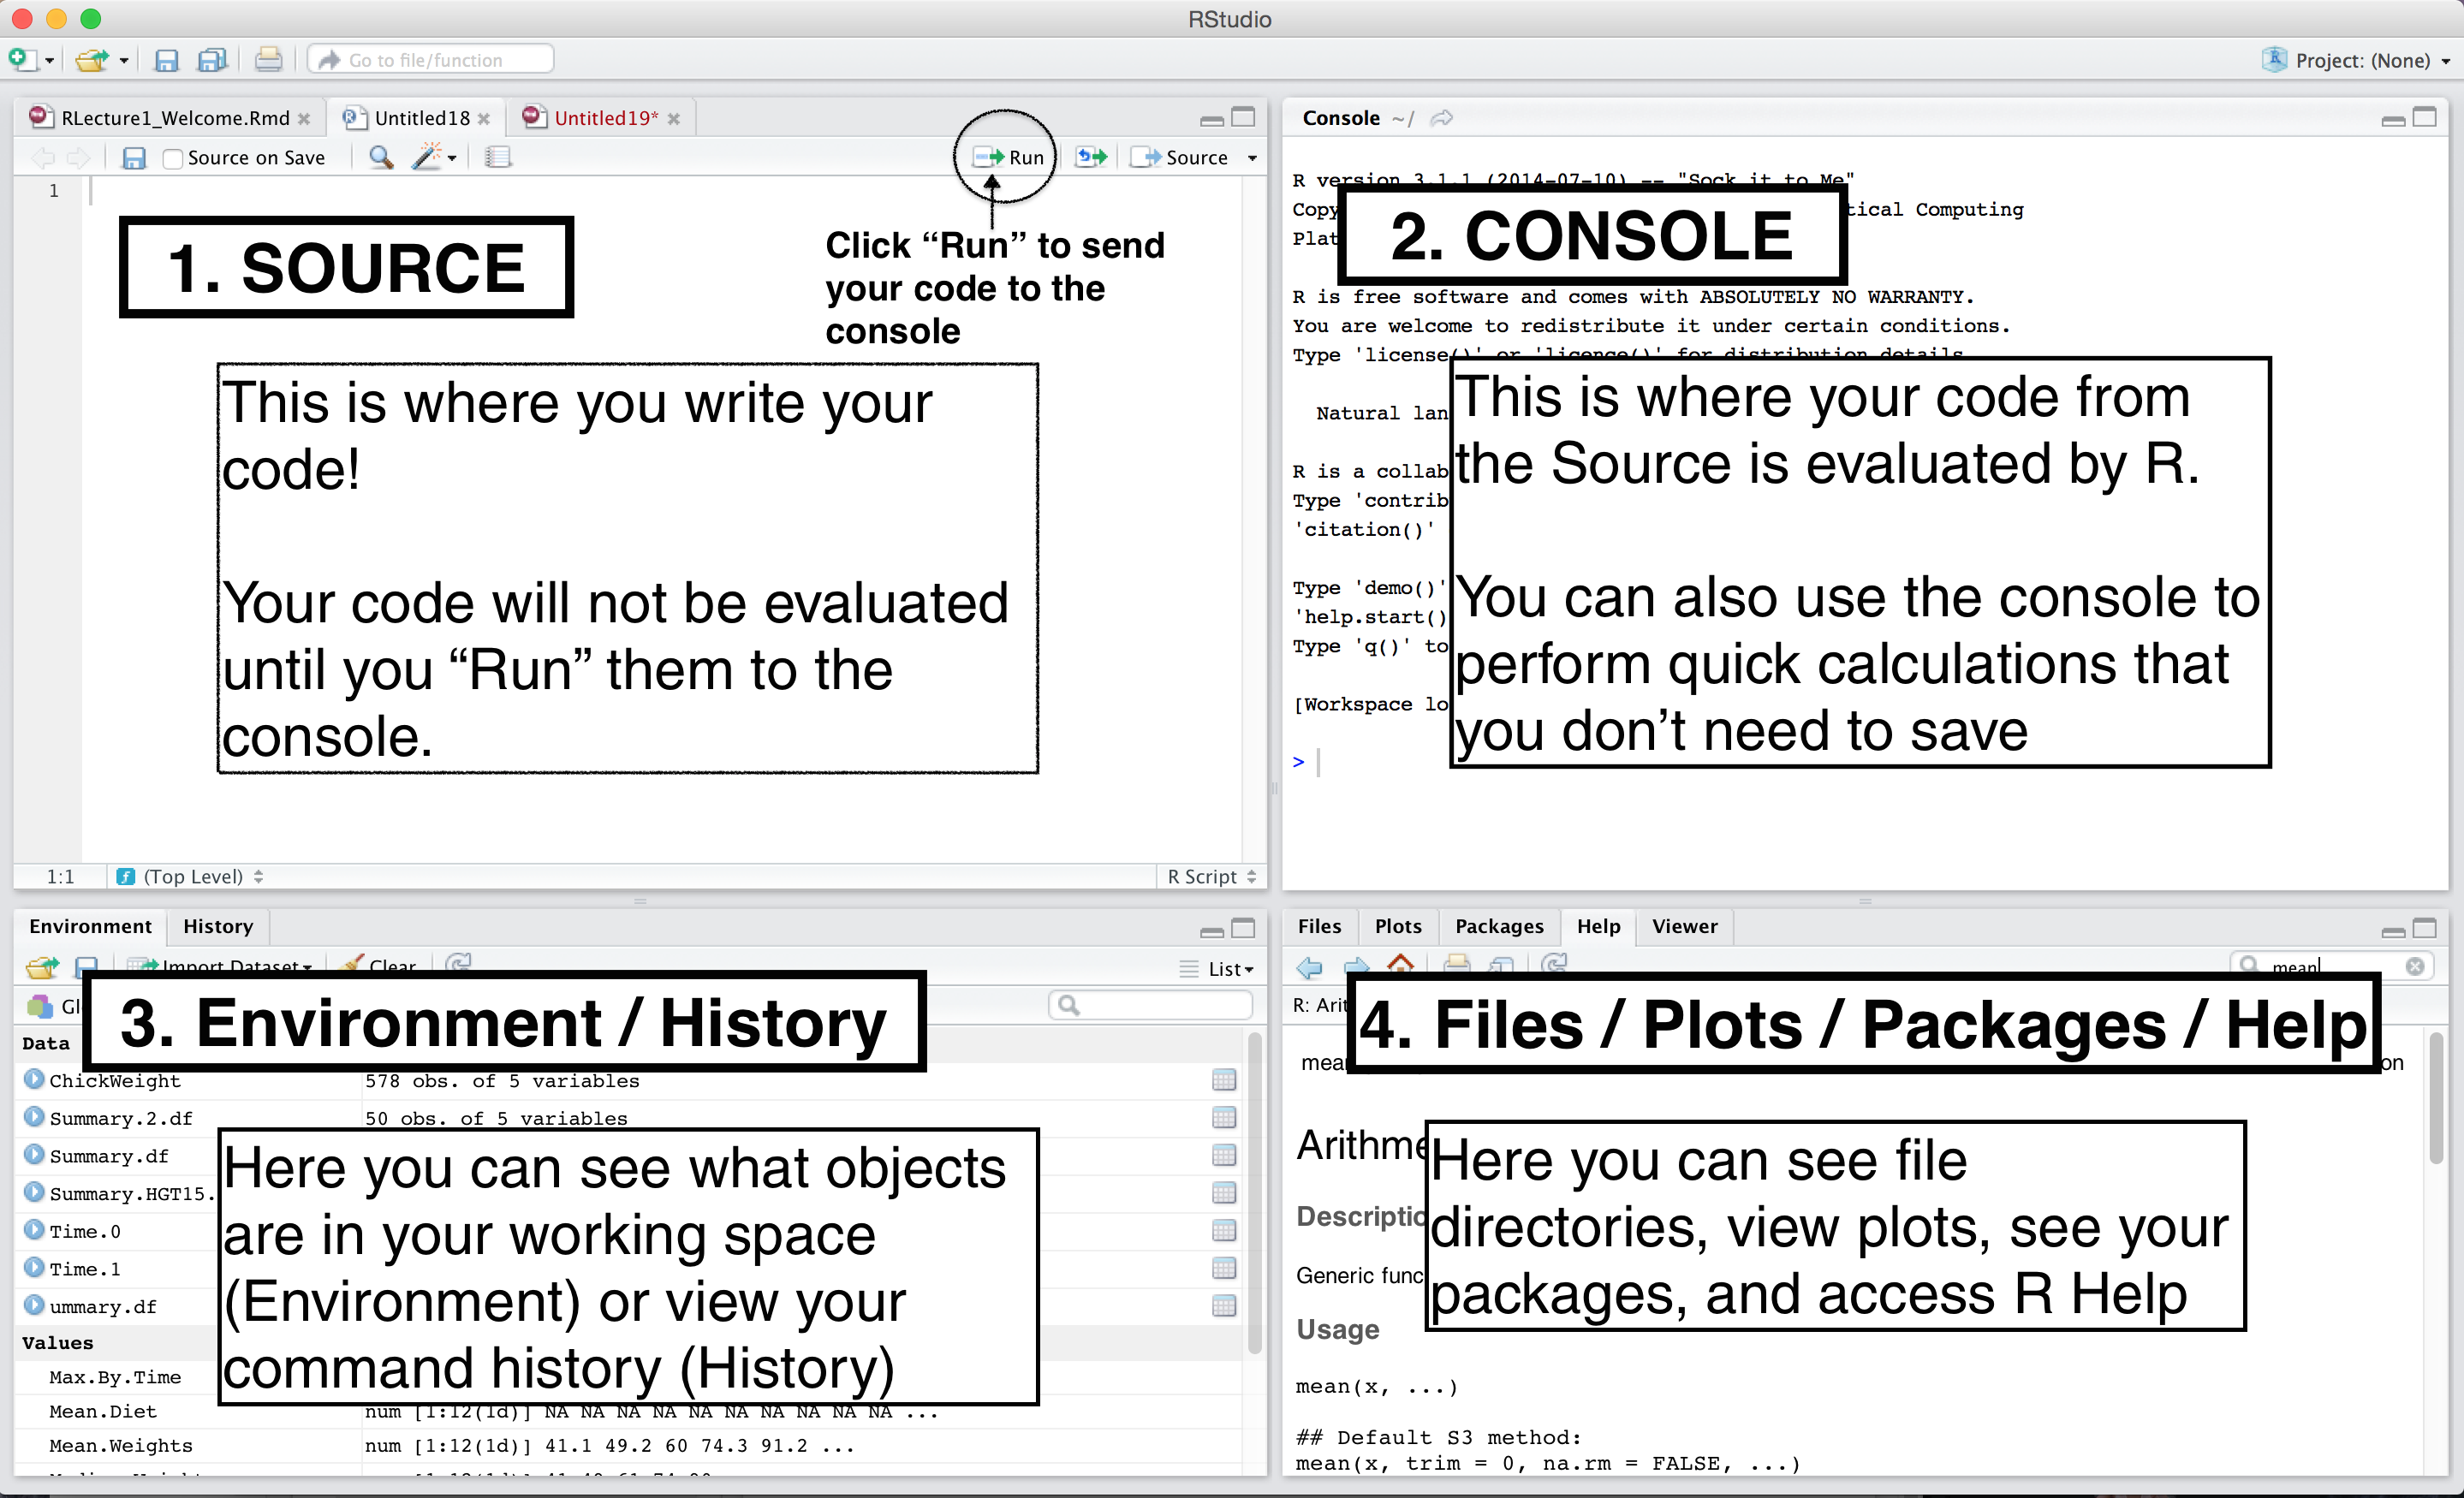
\includegraphics[width=600px]{images/RStudio_Screenshot_Labels} \caption{The four panes of RStudio.}\label{fig:rstudiowindows}
\end{figure}

Now, let's see what each window does in detail.

\subsection{Source - Your notepad for
code}\label{source---your-notepad-for-code}

\begin{figure}
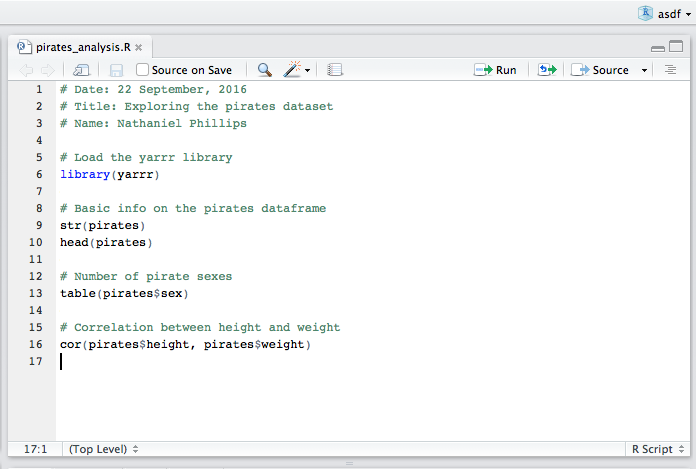
\includegraphics[width=600px]{images/piratesanalysisss} \caption{The Source contains all of your individual R scripts.}\label{fig:sourcewindow}
\end{figure}

The source pane is where you create and edit ``R Scripts" - your
collections of code. Don't worry, R scripts are just text files with the
``.R'' extension. When you open RStudio, it will automatically start a
new Untitled script. Before you start typing in an untitled R script,
you should always save the file under a new file name (like,
``2015PirateSurvey.R''). That way, if something on your computer crashes
while you're working, R will have your code waiting for you when you
re-open RStudio.

You'll notice that when you're typing code in a script in the Source
panel, R won't actually evaluate the code as you type. To have R
actually evaluate your code, you need to first `send' the code to the
Console (we'll talk about this in the next section).

There are many ways to send your code from the Source to the console.
The slowest way is to copy and paste. A faster way is to highlight the
code you wish to evaluate and clicking on the ``Run'' button on the top
right of the Source. Alternatively, you can use the hot-key ``Command +
Return'' on Mac, or ``Control + Enter'' on PC to send all highlighted
code to the console.

\subsection{Console: R's Heart}\label{console-rs-heart}

\begin{figure}
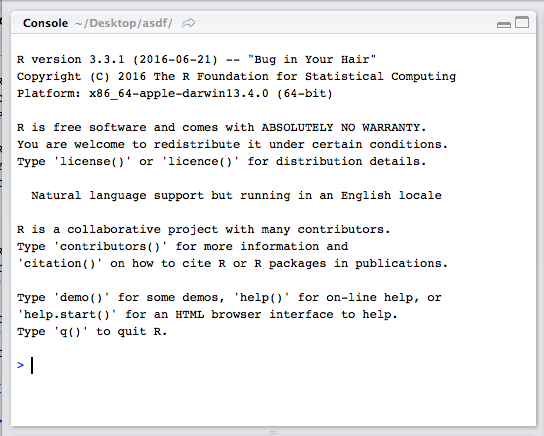
\includegraphics[width=600px]{images/consoless} \caption{The console the calculation heart of R. All of your code will (eventually) go through here.}\label{fig:consolewindow}
\end{figure}

The console is the heart of R. Here is where R actually evaluates code.
At the beginning of the console you'll see the character \texttt{>}.
This is a prompt that tells you that R is ready for new code. You can
type code directly into the console after the \texttt{>} prompt and get
an immediate response. For example, if you type 1+1 into the console and
press enter, you'll see that R immediately gives an output of 2.

\begin{Shaded}
\begin{Highlighting}[]
\DecValTok{1+1}
\end{Highlighting}
\end{Shaded}

\begin{verbatim}
## [1] 2
\end{verbatim}

Try calculating 1+1 by typing the code directly into the console - then
press Enter. You should see the result {[}1{]} 2. Don't worry about the
{[}1{]} for now, we'll get to that later. For now, we're happy if we
just see the 2. Then, type the same code into the Source, and then send
the code to the Console by highlighting the code and clicking the ``Run"
button on the top right hand corner of the Source window. Alternatively,
you can use the hot-key ``Command + Return'' on Mac or ``Control +
Enter'' on Windows.

\textbf{Tip}: Try to write most of your code in a document in the
Source. Only type directly into the Console to de-bug or do quick
analyses.\}

So as you can see, you can execute code either by running it from the
Source or by typing it directly into the Console. However, 99\% most of
the time, you should be using the Source rather than the Console. The
reason for this is straightforward: If you type code into the console,
it won't be saved (though you can look back on your command History).
And if you make a mistake in typing code into the console, you'd have to
re-type everything all over again. Instead, it's better to write all
your code in the Source. When you are ready to execute some code, you
can then send ``Run'' it to the console.

\subsection{Environment / History}\label{environment-history}

\begin{figure}
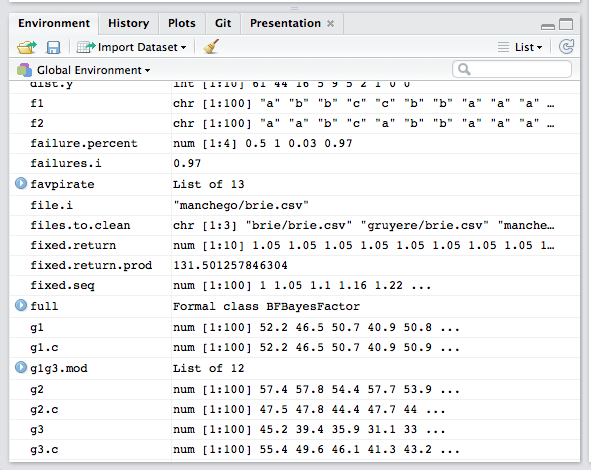
\includegraphics[width=600px]{images/environmentss} \caption{The environment panel shows you all the objects you have defined in your current workspace. You'll learn more about workspaces in Chapter 7.}\label{fig:environment}
\end{figure}

The Environment tab of this panel shows you the names of all the data
objects (like vectors, matrices, and dataframes) that you've defined in
your current R session. You can also see information like the number of
observations and rows in data objects. The tab also has a few clickable
actions like ``Import Dataset" which will open a graphical user
interface (GUI) for important data into R. However, I almost never look
at this menu.

The History tab of this panel simply shows you a history of all the code
you've previously evaluated in the Console. To be honest, I never look
at this. In fact, I didn't realize it was even there until I started
writing this tutorial.

As you get more comfortable with R, you might find the Environment /
History panel useful. But for now you can just ignore it. If you want to
declutter your screen, you can even just minimize the window by clicking
the minimize button on the top right of the panel.

\subsection{Files / Plots / Packages /
Help}\label{files-plots-packages-help}

The Files / Plots / Packages / Help panel shows you lots of helpful
information. Let's go through each tab in detail:

\begin{enumerate}
\def\labelenumi{\arabic{enumi}.}
\item
  Files - The files panel gives you access to the file directory on your
  harddrive. One nice feature of the ``Files'' panel is that you can use
  it to set your working directory - once you navigate to a folder you
  want to read and save files to, click ``More'' and then ``Set As
  Working Directory.'' We'll talk about working directories in more
  detail soon.
\item
  Plots - The Plots panel (no big surprise), shows all your plots. There
  are buttons for opening the plot in a separate window and exporting
  the plot as a pdf or jpeg (though you can also do this with code using
  the \texttt{pdf()} or \texttt{jpeg()} functions.)
\end{enumerate}

Let's see how plots are displayed in the Plots panel. Run the code on
the right to display a histogram of the weights of chickens stored in
the \texttt{ChickWeight} dataset. When you do, you should see a plot
similar to the one in Figure \ref{fig:plotpanel} show up in the Plots
panel.

\begin{Shaded}
\begin{Highlighting}[]
\KeywordTok{hist}\NormalTok{(}\DataTypeTok{x =} \NormalTok{ChickWeight$weight,}
     \DataTypeTok{main =} \StringTok{"Chicken Weights"}\NormalTok{,}
     \DataTypeTok{xlab =} \StringTok{"Weight"}\NormalTok{,}
     \DataTypeTok{col =} \StringTok{"skyblue"}\NormalTok{,}
     \DataTypeTok{border =} \StringTok{"white"}\NormalTok{)}
\end{Highlighting}
\end{Shaded}

\begin{figure}
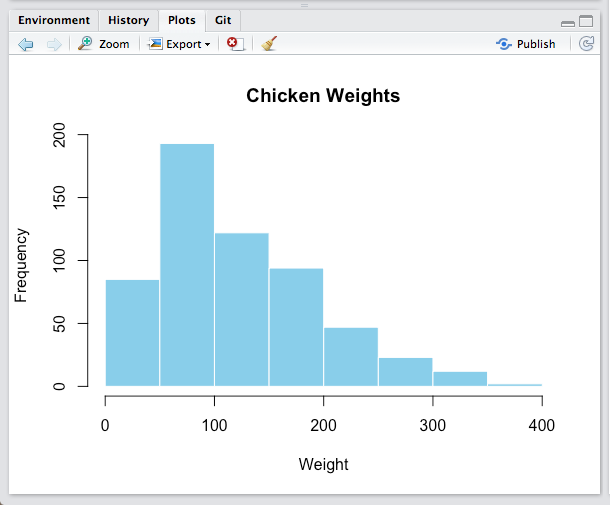
\includegraphics[width=600px]{images/plotpanelss} \caption{The plot panel contains all of your plots, like this histogram of the distribution of chicken weights.}\label{fig:plotpanel}
\end{figure}

\begin{enumerate}
\def\labelenumi{\arabic{enumi}.}
\setcounter{enumi}{2}
\item
  Packages - Shows a list of all the R packages installed on your
  harddrive and indicates whether or not they are currently loaded.
  Packages that are loaded in the current session are checked while
  those that are installed but not yet loaded are unchecked. We'll
  discuss packages in more detail in the next section.
\item
  Help - Help menu for R functions. You can either type the name of a
  function in the search window, or use the code \texttt{?function.name}
  to search for a function with the name \texttt{function.name}
\end{enumerate}

\begin{Shaded}
\begin{Highlighting}[]
\NormalTok{?hist   }\CommentTok{# How does the histogram function work?}
\NormalTok{?t.test }\CommentTok{# What about a t-test?}
\end{Highlighting}
\end{Shaded}

\section{Packages}\label{packages}

When you download and install R for the first time, you are installing
the Base R software. Base R will will contain most of the functions
you'll use on a daily basis like \texttt{mean()} and \texttt{hist()}.
However, only functions written by the original authors of the R
language will appear here. If you want to access data and code written
by other people, you'll need to install it as a \emph{package}. An R
package is simply a bunch of data, from functions, to help menus, to
vignettes (examples), stored in one neat package.

\begin{figure}

{\centering 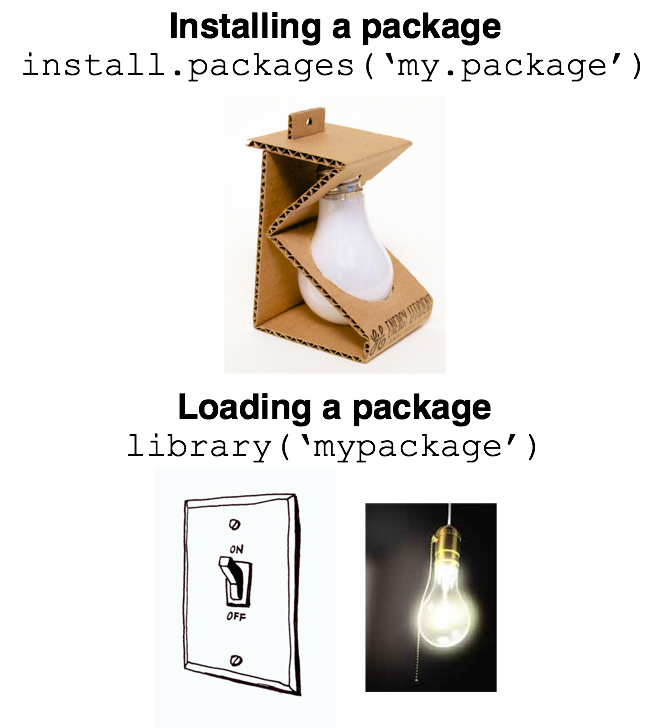
\includegraphics[width=300px]{images/packagebulb} 

}

\caption{An R package is light a lightbulb. First you need to order it with install.packages(). Then, every time you want to use it, you need to turn it on with library()}\label{fig:package}
\end{figure}

A package is like a lightbulb. In order to use it, you first need to
order it to your house (i.e.; your computer) by \emph{installing} it.
Once you've installed a package, you never need to install it again.
However, every time you want to actually use the package, you need to
turn it on by \emph{loading} it. Here's how to do it.

\subsection{Installing a new package}\label{installing-a-new-package}

Installing a package simply means downloading the package code onto your
personal computer. There are two main ways to install new packages. The
first, and most common, method is to download them from the
Comprehensive R Archive Network (CRAN). CRAN is the central repository
for R packages. To install a new R package from CRAN, you can simply run
the code \texttt{install.packages("name")}, where ``name'' is the name
of the package. For example, to download the \texttt{yarrr} package,
which contains several data sets and functions we will use in this book,
you should run the following:

\begin{figure}

{\centering 
\includegraphics[width=200px]{images/cran} 

}

\caption{CRAN (Comprehensive R Archive Network) is the main source of R packages}\label{fig:cran}
\end{figure}

\begin{Shaded}
\begin{Highlighting}[]
\CommentTok{# Install the yarrr package from CRAN}
\CommentTok{#   You only need to install a package once!}
\KeywordTok{install.packages}\NormalTok{(}\StringTok{"yarrr"}\NormalTok{)}
\end{Highlighting}
\end{Shaded}

When you run \texttt{install.packages("name")} R will download the
package from CRAN. If everything works, you should see some information
about where the package is being downloaded from, in addition to a
progress bar.

\begin{figure}

{\centering 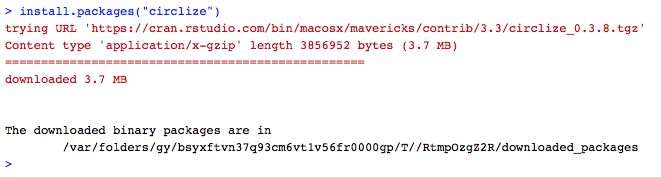
\includegraphics[width=500px]{images/installingpackages} 

}

\caption{When you install a new package, you'll see some random text like this you the download progress. You don't need to memorize this.}\label{fig:installingpackages}
\end{figure}

Like ordering a lightbulb, once you've installed a package on your
computer you never need to install it again (unless you want to try to
install a new version of the package). However, every time you want to
use it, you need to turn it on by loading it.

\subsection{Loading a package}\label{loading-a-package}

Once you've installed a package, it's on your computer. However, just
because it's on your computer doesn't mean R is ready to use it. If you
want to use something, like a function or dataset, from a package you
\emph{always} need to \emph{load} the package in your R session first.
Just like a lightbulb, you need to turn it on to use it!

To load a package, you use the \texttt{library()} function. For example,
now that we've installed the \texttt{yarrr} package, we can load it with
\texttt{library("yarrr")}:

\begin{Shaded}
\begin{Highlighting}[]
\CommentTok{# Load the yarrr package so I can use it!}
\CommentTok{#   You have to load a package in every new R session!}
\KeywordTok{library}\NormalTok{(}\StringTok{"yarrr"}\NormalTok{)}
\end{Highlighting}
\end{Shaded}

Now that you've loaded the \texttt{yarrr} package, you can use any of
its functions! One of the coolest functions in this package is called
\texttt{pirateplot()}. Rather than telling you what a pirateplot is,
let's just make one. Run the following code chunk to make your own
pirateplot. Don't worry about the specifics of the code below, you'll
learn more about how all this works later. For now, just run the code
and marvel at your pirateplot.

\begin{Shaded}
\begin{Highlighting}[]
\CommentTok{# Make a pirateplot using the pirateplot() function}
\CommentTok{#  from the yarrr package!}

\KeywordTok{pirateplot}\NormalTok{(}\DataTypeTok{formula =} \NormalTok{weight ~}\StringTok{ }\NormalTok{Time, }
           \DataTypeTok{data =} \NormalTok{ChickWeight,}
           \DataTypeTok{pal =} \StringTok{"xmen"}\NormalTok{)}
\end{Highlighting}
\end{Shaded}

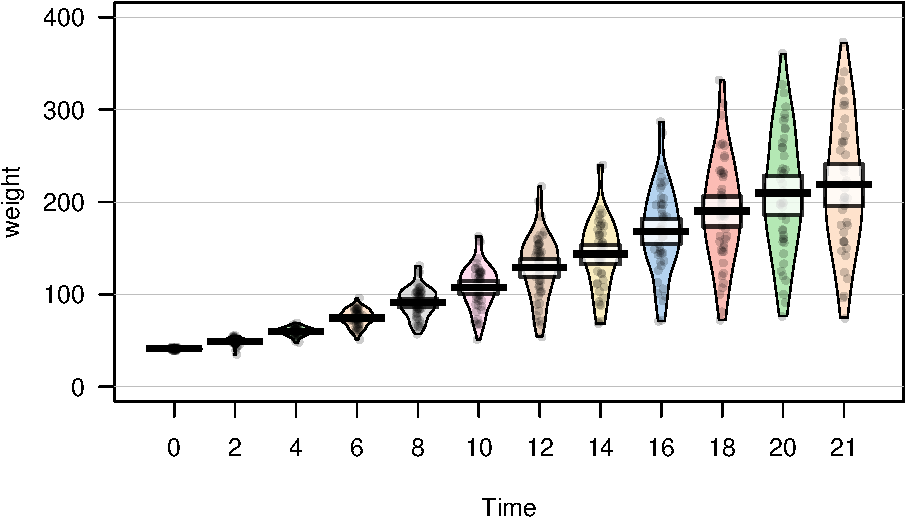
\includegraphics{YaRrr_files/figure-latex/unnamed-chunk-15-1.pdf}

There is one way in R to temporarily load a package without using the
\texttt{library()} function. To do this, you can simply use the notation
\texttt{package::function} notation. This notation simply tells R to
load the package just for this one chunk of code. For example, I could
use the \texttt{pirateplot} function from \texttt{yarrr} package as
follows:

\begin{Shaded}
\begin{Highlighting}[]
\CommentTok{# Use the pirateplot() function without loading the yarrr package first}
\NormalTok{yarrr::}\KeywordTok{pirateplot}\NormalTok{(}\DataTypeTok{formula =} \NormalTok{weight ~}\StringTok{ }\NormalTok{Diet,}
                  \DataTypeTok{data =} \NormalTok{ChickWeight)}
\end{Highlighting}
\end{Shaded}

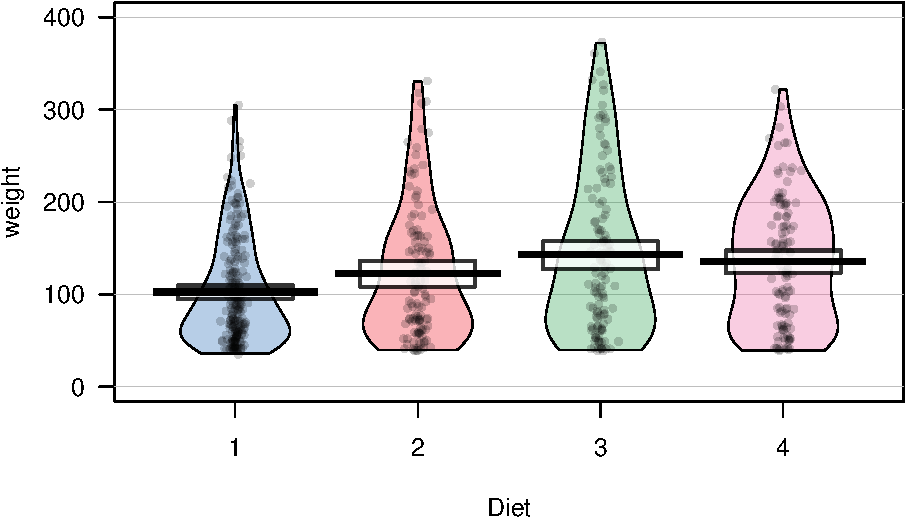
\includegraphics{YaRrr_files/figure-latex/unnamed-chunk-16-1.pdf}

Again, you can think about the \texttt{package::function} method as a
way to temporarily loading a package for a single line of code. One
benefit of using the \texttt{package::function} notation is that it's
immediately clear to anyone reading the code which package contains the
function. However, a drawback is that if you are using a function from a
package often, it forces you to constantly retype the package name. You
can use whichever method makes sense for you.

\section{Cheatsheets and getting
help}\label{cheatsheets-and-getting-help}

\subsection{R Cheatsheets}\label{r-cheatsheets}

\begin{figure}

{\centering 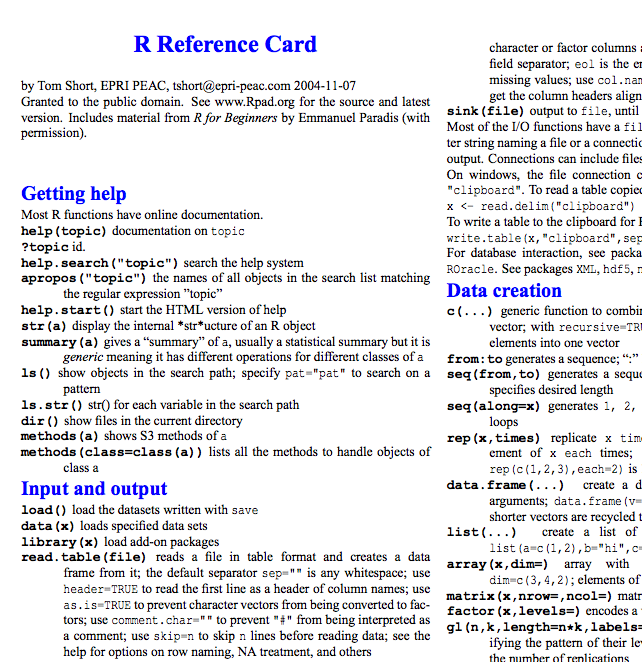
\includegraphics[width=500px]{images/rreferencess} 

}

\caption{The R reference card written by Tom Short is absolutely indispensable!}\label{fig:rreferencecard}
\end{figure}

Over the course of this book, you will be learning \emph{lots} of new
functions. Wouldn't it be nice if someone created a Cheatsheet /
Dictionary of many common R functions? Yes it would, and thankfully
several friendly R programmers have done just that. Below is a table of
some of them that I recommend. I highly encourage you to print these out
and start highlighting functions as you learn them!

\begin{longtable}[]{@{}ll@{}}
\toprule
\begin{minipage}[b]{0.29\columnwidth}\raggedright\strut
CheatSheet\strut
\end{minipage} & \begin{minipage}[b]{0.13\columnwidth}\raggedright\strut
Link\strut
\end{minipage}\tabularnewline
\midrule
\endhead
\begin{minipage}[t]{0.29\columnwidth}\raggedright\strut
R Basics by Tom Short\strut
\end{minipage} & \begin{minipage}[t]{0.13\columnwidth}\raggedright\strut
\url{https://cran.r-project.org/doc/contrib/Short-refcard.pdf}\strut
\end{minipage}\tabularnewline
\begin{minipage}[t]{0.29\columnwidth}\raggedright\strut
R Basics by Mhairi McNeill\strut
\end{minipage} & \begin{minipage}[t]{0.13\columnwidth}\raggedright\strut
\url{http://github.com/rstudio/cheatsheets/raw/master/source/pdfs/base-r.pdf}\strut
\end{minipage}\tabularnewline
\begin{minipage}[t]{0.29\columnwidth}\raggedright\strut
Advanced R by Arianne Colton and Sean Chen\strut
\end{minipage} & \begin{minipage}[t]{0.13\columnwidth}\raggedright\strut
\href{https://www.rstudio.com/wp-content/uploads/2016/02/advancedR.pdf}{hhttps://www.rstudio.com/wp-content/uploads/2016/02/advancedR.pdf}\strut
\end{minipage}\tabularnewline
\begin{minipage}[t]{0.29\columnwidth}\raggedright\strut
Plotting\strut
\end{minipage} & \begin{minipage}[t]{0.13\columnwidth}\raggedright\strut
\url{https://www.rstudio.com/wp-content/uploads/2016/10/how-big-is-your-graph.pdf}\strut
\end{minipage}\tabularnewline
\bottomrule
\end{longtable}

\subsection{Getting R help online}\label{getting-r-help-online}

Here are some resources for R help and inspiration that I can highly
recommend

\begin{enumerate}
\def\labelenumi{\arabic{enumi}.}
\item
  \url{http://www.r-bloggers.com}: R bloggers is my go-to place to
  discover the latest and greatest with R.
\item
  \url{http://blog.revolutionanalytics.com}: Revolution analytics always
  has great R related material.
\item
  \url{http://www.kaggle.com}: Kaggle is a really cool website that
  posts data analysis challenges that anyone can try to solve. It also
  contains a wide range of real-world datasets and tutorials.
\item
  \url{https://www.r-bloggers.com/learning-statistics-on-youtube/}: If
  you like to learn with YouTube, this page contains many links to R
  related YouTube channels.
\end{enumerate}

\chapter{Jump In!}\label{jumpin}

\begin{figure}

{\centering 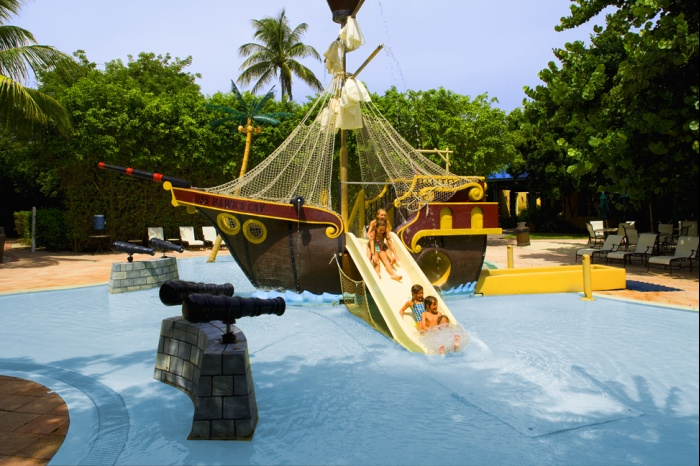
\includegraphics[width=400px]{images/pirateswimming} 

}

\caption{Despite what you might find at family friendly waterparks -- this is NOT how real pirate swimming lessons look.}\label{fig:unnamed-chunk-18}
\end{figure}

What's the first exercise on the first day of pirate swimming lessons?
While it would be cute if they all had little inflatible pirate ships to
swim around in -- unfortunately this is not the case. Instead, those
baby pirates take a walk off their baby planks so they can get a taste
of what they're in for. Turns out, learning R is the same way. Let's
jump in. In this chapter, you'll see how easy it is to calculate basic
statistics and create plots in R. Don't worry if the code you're running
doesn't make immediate sense -- just marvel at how easy it is to do this
in R!

In this section, we'll analyze a dataset called\ldots{}wait for
it\ldots{}pirates! The dataset contains data from a survey of 1,000
pirates. The data is contained in the \texttt{yarrr} package, so make
sure you've installed and loaded the package:

\begin{Shaded}
\begin{Highlighting}[]
\CommentTok{# Install the yarrr package}
\KeywordTok{install.packages}\NormalTok{(}\StringTok{'yarrr'}\NormalTok{)}

\CommentTok{# Load the package}
\KeywordTok{library}\NormalTok{(yarrr)}
\end{Highlighting}
\end{Shaded}

\section{Exploring data}\label{exploring-data}

Next, we'll look at the help menu for the pirates dataset using the
question mark \texttt{?pirates}. When you run this, you should see a
small help window open up in RStudio that gives you some information
about the dataset.

\begin{Shaded}
\begin{Highlighting}[]
\NormalTok{?pirates}
\end{Highlighting}
\end{Shaded}

First, let's take a look at the first few rows of the dataset using the
\texttt{head()} function. This will show you the first few rows of the
data.

\begin{Shaded}
\begin{Highlighting}[]
\CommentTok{# Look at the first few rows of the data}
\KeywordTok{head}\NormalTok{(pirates)}
\NormalTok{##   id    sex age height weight headband college tattoos tchests parrots}
\NormalTok{## 1  1   male  28    173     70      yes   JSSFP       9       0       0}
\NormalTok{## 2  2   male  31    209    106      yes   JSSFP       9      11       0}
\NormalTok{## 3  3   male  26    170     77      yes    CCCC      10      10       1}
\NormalTok{## 4  4 female  31    144     58       no   JSSFP       2       0       2}
\NormalTok{## 5  5 female  41    158     58      yes   JSSFP       9       6       4}
\NormalTok{## 6  6   male  26    190     85      yes    CCCC       7      19       0}
\NormalTok{##   favorite.pirate sword.type eyepatch sword.time beard.length}
\NormalTok{## 1    Jack Sparrow    cutlass        1       0.58           16}
\NormalTok{## 2    Jack Sparrow    cutlass        0       1.11           21}
\NormalTok{## 3    Jack Sparrow    cutlass        1       1.44           19}
\NormalTok{## 4    Jack Sparrow   scimitar        1      36.11            2}
\NormalTok{## 5            Hook    cutlass        1       0.11            0}
\NormalTok{## 6    Jack Sparrow    cutlass        1       0.59           17}
\NormalTok{##             fav.pixar grogg}
\NormalTok{## 1      Monsters, Inc.    11}
\NormalTok{## 2              WALL-E     9}
\NormalTok{## 3          Inside Out     7}
\NormalTok{## 4          Inside Out     9}
\NormalTok{## 5          Inside Out    14}
\NormalTok{## 6 Monsters University     7}
\end{Highlighting}
\end{Shaded}

You can look at the names of the columns in the dataset with the
\texttt{names()} function

\begin{Shaded}
\begin{Highlighting}[]
\CommentTok{# What are the names of the columns?}
\KeywordTok{names}\NormalTok{(pirates)}
\NormalTok{##  [1] "id"              "sex"             "age"            }
\NormalTok{##  [4] "height"          "weight"          "headband"       }
\NormalTok{##  [7] "college"         "tattoos"         "tchests"        }
\NormalTok{## [10] "parrots"         "favorite.pirate" "sword.type"     }
\NormalTok{## [13] "eyepatch"        "sword.time"      "beard.length"   }
\NormalTok{## [16] "fav.pixar"       "grogg"}
\end{Highlighting}
\end{Shaded}

Finally, you can also view the entire dataset in a separate window using
the \texttt{View()} function:

\begin{Shaded}
\begin{Highlighting}[]
\CommentTok{# View the entire dataset in a new window}
\KeywordTok{View}\NormalTok{(pirates)}
\end{Highlighting}
\end{Shaded}

\section{Descriptive statistics}\label{descriptive-statistics}

Now let's calculate some basic statistics on the entire dataset. We'll
calculate the mean age, maximum height, and number of pirates of each
sex:

\begin{Shaded}
\begin{Highlighting}[]
\CommentTok{# What is the mean age?}
\KeywordTok{mean}\NormalTok{(pirates$age)}
\NormalTok{## [1] 27}

\CommentTok{# What was the tallest pirate?}
\KeywordTok{max}\NormalTok{(pirates$height)}
\NormalTok{## [1] 209}

\CommentTok{# How many pirates are there of each sex?}
\KeywordTok{table}\NormalTok{(pirates$sex)}
\NormalTok{## }
\NormalTok{## female   male  other }
\NormalTok{##    464    490     46}
\end{Highlighting}
\end{Shaded}

Now, let's calculate statistics for different groups of pirates. For
example, the following code will use the \texttt{aggregate()} function
to calculate the mean age of pirates, separately for each sex.

\begin{Shaded}
\begin{Highlighting}[]
\CommentTok{# Calculate the mean age, separately for each sex}
\KeywordTok{aggregate}\NormalTok{(}\DataTypeTok{formula =} \NormalTok{age ~}\StringTok{ }\NormalTok{sex,}
          \DataTypeTok{data =} \NormalTok{pirates,}
          \DataTypeTok{FUN =} \NormalTok{mean)}
\NormalTok{##      sex age}
\NormalTok{## 1 female  30}
\NormalTok{## 2   male  25}
\NormalTok{## 3  other  27}
\end{Highlighting}
\end{Shaded}

\section{Plotting}\label{plotting}

Cool stuff, now let's make a plot! We'll plot the relationship between
pirate's height and weight using the \texttt{plot()} function. We'll
also include a blue regression line to measure the strength of the
relationship.

\begin{Shaded}
\begin{Highlighting}[]
\CommentTok{# Create scatterplot}
\KeywordTok{plot}\NormalTok{(}\DataTypeTok{x =} \NormalTok{pirates$height,        }\CommentTok{# X coordinates}
     \DataTypeTok{y =} \NormalTok{pirates$weight,        }\CommentTok{# y-coordinates}
     \DataTypeTok{main =} \StringTok{'My first scatterplot of pirate data!'}\NormalTok{,}
     \DataTypeTok{xlab =} \StringTok{'Height (in cm)'}\NormalTok{,   }\CommentTok{# x-axis label}
     \DataTypeTok{ylab =} \StringTok{'Weight (in kg)'}\NormalTok{,   }\CommentTok{# y-axis label}
     \DataTypeTok{pch =} \DecValTok{16}\NormalTok{,                  }\CommentTok{# Filled circles}
     \DataTypeTok{col =} \KeywordTok{gray}\NormalTok{(.}\DecValTok{0}\NormalTok{, .}\DecValTok{1}\NormalTok{))        }\CommentTok{# Transparent gray}

\KeywordTok{grid}\NormalTok{()        }\CommentTok{# Add gridlines}

\CommentTok{# Create a linear regression model}
\NormalTok{model <-}\StringTok{ }\KeywordTok{lm}\NormalTok{(}\DataTypeTok{formula =} \NormalTok{weight ~}\StringTok{ }\NormalTok{height, }
            \DataTypeTok{data =} \NormalTok{pirates)}

\KeywordTok{abline}\NormalTok{(model, }\DataTypeTok{col =} \StringTok{'blue'}\NormalTok{)      }\CommentTok{# Add regression to plot}
\end{Highlighting}
\end{Shaded}

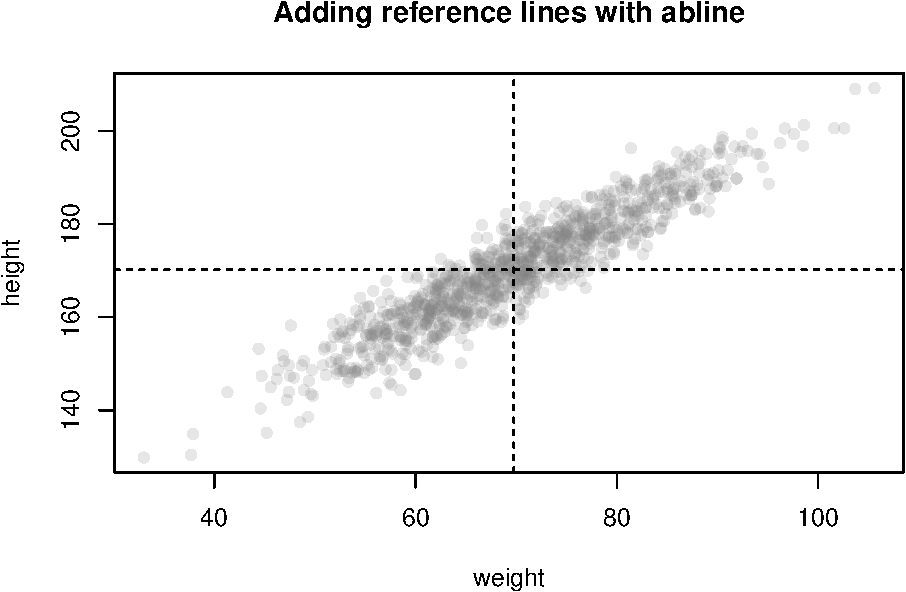
\includegraphics{YaRrr_files/figure-latex/unnamed-chunk-26-1.pdf}

Scatterplots are great for showing the relationship between two
continuous variables, but what if your independent variable is not
continuous? In this case, pirateplots are a good option. Let's create a
pirateplot using the \texttt{pirateplot()} function to show the
distribution of pirate's age based on their favorite sword:

\begin{Shaded}
\begin{Highlighting}[]
\KeywordTok{pirateplot}\NormalTok{(}\DataTypeTok{formula =} \NormalTok{age ~}\StringTok{ }\NormalTok{sword.type, }
           \DataTypeTok{data =} \NormalTok{pirates,}
           \DataTypeTok{main =} \StringTok{"Pirateplot of ages by favorite sword"}\NormalTok{)}
\end{Highlighting}
\end{Shaded}

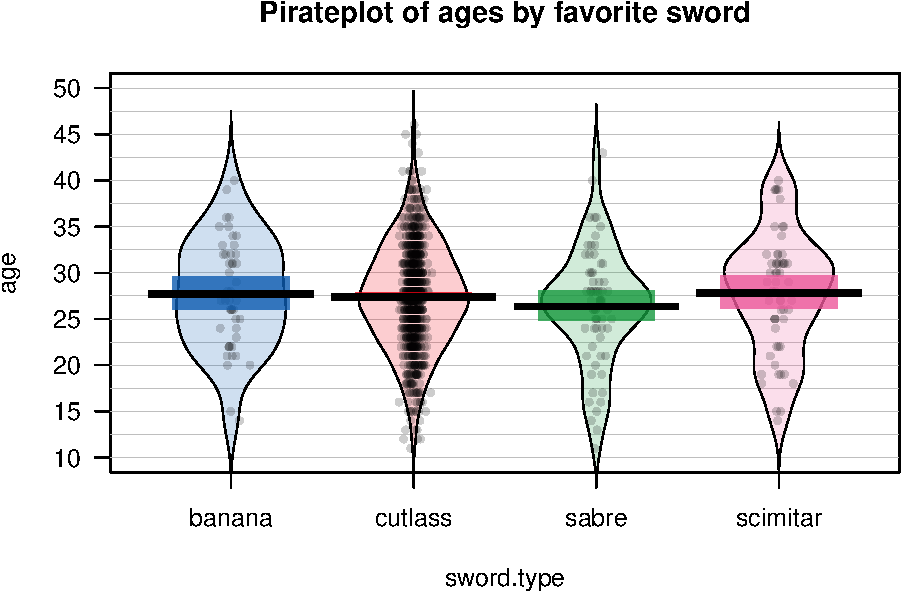
\includegraphics{YaRrr_files/figure-latex/unnamed-chunk-27-1.pdf}

\section{Hypothesis tests}\label{hypothesis-tests}

Now, let's do some basic hypothesis tests. First, let's conduct a
two-sample t-test to see if there is a significant difference between
the ages of pirates who do wear a headband, and those who do not:

\begin{Shaded}
\begin{Highlighting}[]
\CommentTok{# Age by headband t-test}
\KeywordTok{t.test}\NormalTok{(}\DataTypeTok{formula =} \NormalTok{age ~}\StringTok{ }\NormalTok{headband,}
       \DataTypeTok{data =} \NormalTok{pirates,}
       \DataTypeTok{alternative =} \StringTok{'two.sided'}\NormalTok{)}
\NormalTok{## }
\NormalTok{##  Welch Two Sample t-test}
\NormalTok{## }
\NormalTok{## data:  age by headband}
\NormalTok{## t = 0.4, df = 100, p-value = 0.7}
\NormalTok{## alternative hypothesis: true difference in means is not equal to 0}
\NormalTok{## 95 percent confidence interval:}
\NormalTok{##  -1.0  1.5}
\NormalTok{## sample estimates:}
\NormalTok{##  mean in group no mean in group yes }
\NormalTok{##                28                27}
\end{Highlighting}
\end{Shaded}

With a p-value of 0.7259, we don't have sufficient evidence say there is
a difference in the men age of pirates who wear headbands and those that
do not.

Next, let's test if there a significant correlation between a pirate's
height and weight using the \texttt{cor.test()} function:

\begin{Shaded}
\begin{Highlighting}[]
\KeywordTok{cor.test}\NormalTok{(}\DataTypeTok{formula =} \NormalTok{~}\StringTok{ }\NormalTok{height +}\StringTok{ }\NormalTok{weight,}
         \DataTypeTok{data =} \NormalTok{pirates)}
\NormalTok{## }
\NormalTok{##  Pearson's product-moment correlation}
\NormalTok{## }
\NormalTok{## data:  height and weight}
\NormalTok{## t = 80, df = 1000, p-value <2e-16}
\NormalTok{## alternative hypothesis: true correlation is not equal to 0}
\NormalTok{## 95 percent confidence interval:}
\NormalTok{##  0.92 0.94}
\NormalTok{## sample estimates:}
\NormalTok{##  cor }
\NormalTok{## 0.93}
\end{Highlighting}
\end{Shaded}

We got a p-value of \texttt{p\ \textless{}\ 2.2e-16}, that's scientific
notation for \texttt{p\ \textless{}\ .00000000000000016} -- which is
pretty much 0. Thus, we'd conclude that there is a significant
(positive) relationship between a pirate's height and weight.

Now, let's do an ANOVA testing if there is a difference between the
number of tattoos pirates have based on their favorite sword

\begin{Shaded}
\begin{Highlighting}[]
\CommentTok{# Create tattoos model}
\NormalTok{tat.sword.lm <-}\StringTok{ }\KeywordTok{lm}\NormalTok{(}\DataTypeTok{formula =} \NormalTok{tattoos ~}\StringTok{ }\NormalTok{sword.type,}
                   \DataTypeTok{data =} \NormalTok{pirates)}

\CommentTok{# Get ANOVA table}
\KeywordTok{anova}\NormalTok{(tat.sword.lm)}
\NormalTok{## Analysis of Variance Table}
\NormalTok{## }
\NormalTok{## Response: tattoos}
\NormalTok{##             Df Sum Sq Mean Sq F value Pr(>F)    }
\NormalTok{## sword.type   3   1588     529    54.1 <2e-16 ***}
\NormalTok{## Residuals  996   9743      10                   }
\NormalTok{## ---}
\NormalTok{## Signif. codes:  0 '***' 0.001 '**' 0.01 '*' 0.05 '.' 0.1 ' ' 1}
\end{Highlighting}
\end{Shaded}

Sure enough, we see another very small p-value of
\texttt{p\ \textless{}\ 2.2e-16}, suggesting that the number of tattoos
pirate's have are different based on their favorite sword.

\section{Regression}\label{regression}

Finally, let's run a regression analysis to see if a pirate's age,
weight, and number of tattoos (s)he has predicts how many treasure
chests he/she's found:

\begin{Shaded}
\begin{Highlighting}[]
\CommentTok{# Create a linear regression model: DV = tchests, IV = age, weight, tattoos}
\NormalTok{tchests.model <-}\StringTok{ }\KeywordTok{lm}\NormalTok{(}\DataTypeTok{formula =} \NormalTok{tchests ~}\StringTok{ }\NormalTok{age +}\StringTok{ }\NormalTok{weight +}\StringTok{ }\NormalTok{tattoos,}
                    \DataTypeTok{data =} \NormalTok{pirates)}

\CommentTok{# Show summary statistics}
\KeywordTok{summary}\NormalTok{(tchests.model)}
\NormalTok{## }
\NormalTok{## Call:}
\NormalTok{## lm(formula = tchests ~ age + weight + tattoos, data = pirates)}
\NormalTok{## }
\NormalTok{## Residuals:}
\NormalTok{##    Min     1Q Median     3Q    Max }
\NormalTok{## -33.30 -15.83  -6.86   8.41 119.97 }
\NormalTok{## }
\NormalTok{## Coefficients:}
\NormalTok{##             Estimate Std. Error t value Pr(>|t|)    }
\NormalTok{## (Intercept)   5.1908     7.1844    0.72     0.47    }
\NormalTok{## age           0.7818     0.1344    5.82    8e-09 ***}
\NormalTok{## weight       -0.0901     0.0718   -1.25     0.21    }
\NormalTok{## tattoos       0.2540     0.2255    1.13     0.26    }
\NormalTok{## ---}
\NormalTok{## Signif. codes:  0 '***' 0.001 '**' 0.01 '*' 0.05 '.' 0.1 ' ' 1}
\NormalTok{## }
\NormalTok{## Residual standard error: 24 on 996 degrees of freedom}
\NormalTok{## Multiple R-squared:  0.0406, Adjusted R-squared:  0.0377 }
\NormalTok{## F-statistic:   14 on 3 and 996 DF,  p-value: 5.75e-09}
\end{Highlighting}
\end{Shaded}

It looks like the only significant predictor of the number of treasure
chests that a pirate has found is his/her age. There does not seem to be
significant effect of weight or tattoos.

\section{Bayesian Statistics}\label{bayesian-statistics}

Now, let's repeat some of our previous analyses with Bayesian versions.
First we'll install and load the \texttt{BayesFactor} package which
contains the Bayesian statistics functions we'll use:

\begin{Shaded}
\begin{Highlighting}[]
\CommentTok{# Install and load the BayesFactor package}
\KeywordTok{install.packages}\NormalTok{(}\StringTok{'BayesFactor'}\NormalTok{)}
\KeywordTok{library}\NormalTok{(BayesFactor)}
\end{Highlighting}
\end{Shaded}

Now that the packages is installed and loaded, we're good to go! Let's
do a Bayesian version of our earlier t-test asking if pirates who wear a
headband are older or younger than those who do not.

\begin{Shaded}
\begin{Highlighting}[]
\CommentTok{# Bayesian t-test comparing the age of pirates with and without headbands}
\KeywordTok{ttestBF}\NormalTok{(}\DataTypeTok{formula =} \NormalTok{age ~}\StringTok{ }\NormalTok{headband,}
        \DataTypeTok{data =} \NormalTok{pirates)}
\NormalTok{## Bayes factor analysis}
\NormalTok{## --------------}
\NormalTok{## [1] Alt., r=0.707 : 0.12 ±0%}
\NormalTok{## }
\NormalTok{## Against denominator:}
\NormalTok{##   Null, mu1-mu2 = 0 }
\NormalTok{## ---}
\NormalTok{## Bayes factor type: BFindepSample, JZS}
\end{Highlighting}
\end{Shaded}

It looks like we got a Bayes factor of 0.12 which is strong evidence
\emph{for} the null hypothesis (that the mean age does not differ
between pirates with and without headbands)

\section{Wasn't that easy?!}\label{wasnt-that-easy}

Wait\ldots{}wait\ldots{}WAIT! Did you seriously just calculate
descriptive statistics, a t-test, an ANOVA, and a regression, create a
scatterplot and a pirateplot, AND do both a Bayesian t-test and
regression analysis. Yup. Imagine how long it would have taken to
explain how to do all that in SPSS. And while you haven't really learned
how R works yet, I'd bet my beard that you could easily alter the
previous code to do lots of other analyses. Of course, don't worry if
some or all of the previous code didn't make sense. Soon\ldots{}it will
all be clear.

Now that you've jumped in, let's learn how to swim.

\chapter{The Basics}\label{basics}

If you're like most people, you think of R as a statistics program.
However, while R is definitely the coolest, most badass, pirate-y way to
conduct statistics -- it's not really a program. Rather, it's a
programming \textit{language} that was written by and for statisticians.
To learn more about the history of R\ldots{}just\ldots{}you
know\ldots{}Google it.

\begin{figure}

{\centering 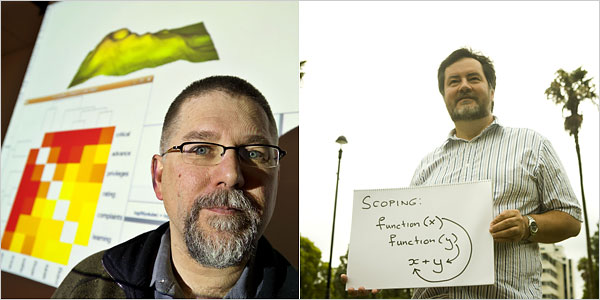
\includegraphics[width=400px]{images/rauthors} 

}

\caption{Ross Ihaka and Robert Gentlemen. You have these two pirates to thank for creating R! You might not think much of them now, but by the end of this book there's a good chance you'll be dressing up as one of them on Halloween.}\label{fig:unnamed-chunk-35}
\end{figure}

In this chapter, we'll go over the basics of the R language and the
RStudio programming environment.

\section{The command-line (Console)}\label{the-command-line-console}

\begin{figure}

{\centering 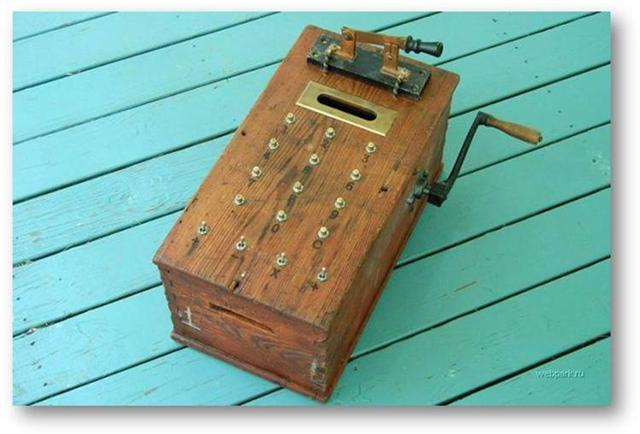
\includegraphics[width=400px]{images/woodcalc} 

}

\caption{Yep. R is really just a fancy calculator. This R programming device was found on a shipwreck on the Bodensee in Germany. I stole it from a museum and made a pretty sweet plot with it. But I don't want to show it to you.}\label{fig:unnamed-chunk-36}
\end{figure}

R code, on its own, is just text. You can write R code in a new script
within R or RStudio, or in any text editor. Hell, you can write R code
on Twitter if you want. However, just writing the code won't do the
whole job -- in order for your code to be executed (aka, interpreted)
you need to send it to R's \textit{command-line interpreter}. In
RStudio, the command-line interpreter is called the Console.

\begin{figure}

{\centering 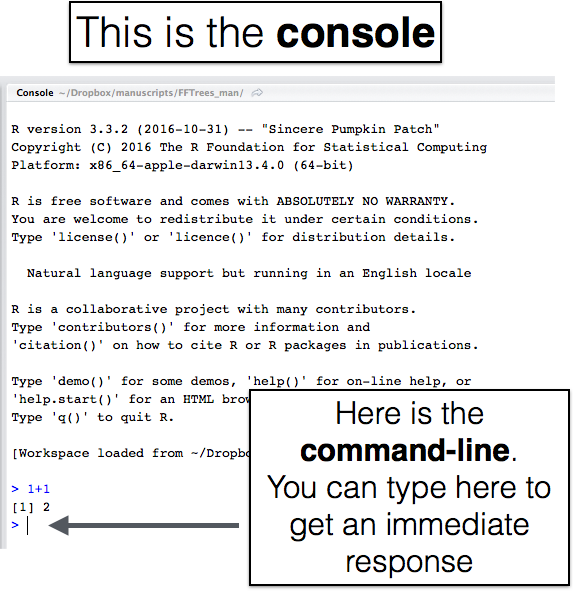
\includegraphics[width=600px]{images/commandline} 

}

\caption{You can always type code directly into the command line to get an immediate response.}\label{fig:unnamed-chunk-37}
\end{figure}

In R, the command-line interpreter starts with the \textgreater{}
symbol. This is called the \textit{prompt}. Why is it called the prompt?
Well, it's ``prompting'' you to feed it with some R code. The fastest
way to have R evaluate code is to type your R code directly into the
command-line interpreter. For example, if you type \texttt{1+1} into the
interpreter and hit enter you'll see the following

\begin{Shaded}
\begin{Highlighting}[]
\DecValTok{1+1}
\NormalTok{## [1] 2}
\end{Highlighting}
\end{Shaded}

As you can see, R returned the (thankfully correct) value of 2. You'll
notice that the console also returns the text {[}1{]}. This is just
telling you you the index of the value next to it. Don't worry about
this for now, it will make more sense later. As you can see, R can,
thankfully, do basic calculations. In fact, at its heart, R is
technically just a fancy calculator. But that's like saying Michael
Jordan is \emph{just} a fancy ball bouncer or Donald Trump is
\emph{just} a orange with a dead fox on his head. It (and they), are
much more than that.

\section{Writing R scripts in an
editor}\label{writing-r-scripts-in-an-editor}

There are certainly many cases where it makes sense to type code
directly into the console. For example, to open a help menu for a new
function with the ? command, to take a quick look at a dataset with the
\texttt{head()} function, or to do simple calculations like
\texttt{1+1}, you should type directly into the console. However, the
problem with writing all your code in the console is that nothing that
you write will be saved. So if you make an error, or want to make a
change to some earlier code, you have to type it all over again. Not
very efficient. For this (and many more reasons), you'll should write
any important code that you want to save as an R script. An R script is
just a bunch of R code in a single file. You can write an R script in
any text editor, but you should save it with the \texttt{.R} suffix to
make it clear that it contains R code.\} in an editor.

In RStudio, you'll write your R code in the\ldots{}wait for
it\ldots{}\emph{Source} window. To start writing a new R script in
RStudio, click File -- New File -- R Script.

\textbf{Shortcut!} To create a new script in R, you can also use the
command--shift--N shortcut on Mac. I don't know what it is on
PC\ldots{}and I don't want to know.

When you open a new script, you'll see a blank page waiting for you to
write as much R code as you'd like. In Figure \ref{fig:editor}, I have a
new script called \texttt{examplescript} with a few random calculations.

\begin{figure}

{\centering 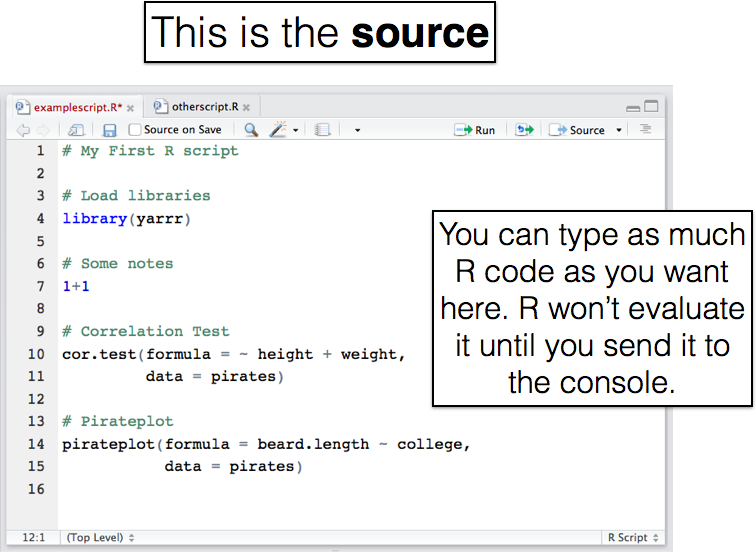
\includegraphics[width=600px]{images/sourcess} 

}

\caption{Here's how a new script looks in the editor window on RStudio. The code you type won't be executed until you send it to the console.}\label{fig:editor}
\end{figure}

You can have several R scripts open in the source window in separate
tabs (like I have above).

\subsection{Send code from an editor to the
console}\label{send-code-from-an-editor-to-the-console}

When you type code into an R script, you'll notice that, unlike typing
code into the Console, nothing happens. In order for R to interpret the
code, you need to send it from the Editor to the Console. There are a
few ways to do this, here are the three most common ways:

\begin{enumerate}
\def\labelenumi{\arabic{enumi}.}
\item
  Copy the code from the Editor (or anywhere that has valid R code), and
  paste it into the Console (using Command--V).
\item
  Highlight the code you want to run (with your mouse or by holding
  Shift), then use the Command--Return shortcut (see Figure
  \ref{fig:commandreturn}).
\item
  Place the cursor on a single line you want to run, then use the
  Command--Return shortcut to run just that line.
\end{enumerate}

\begin{figure}

{\centering 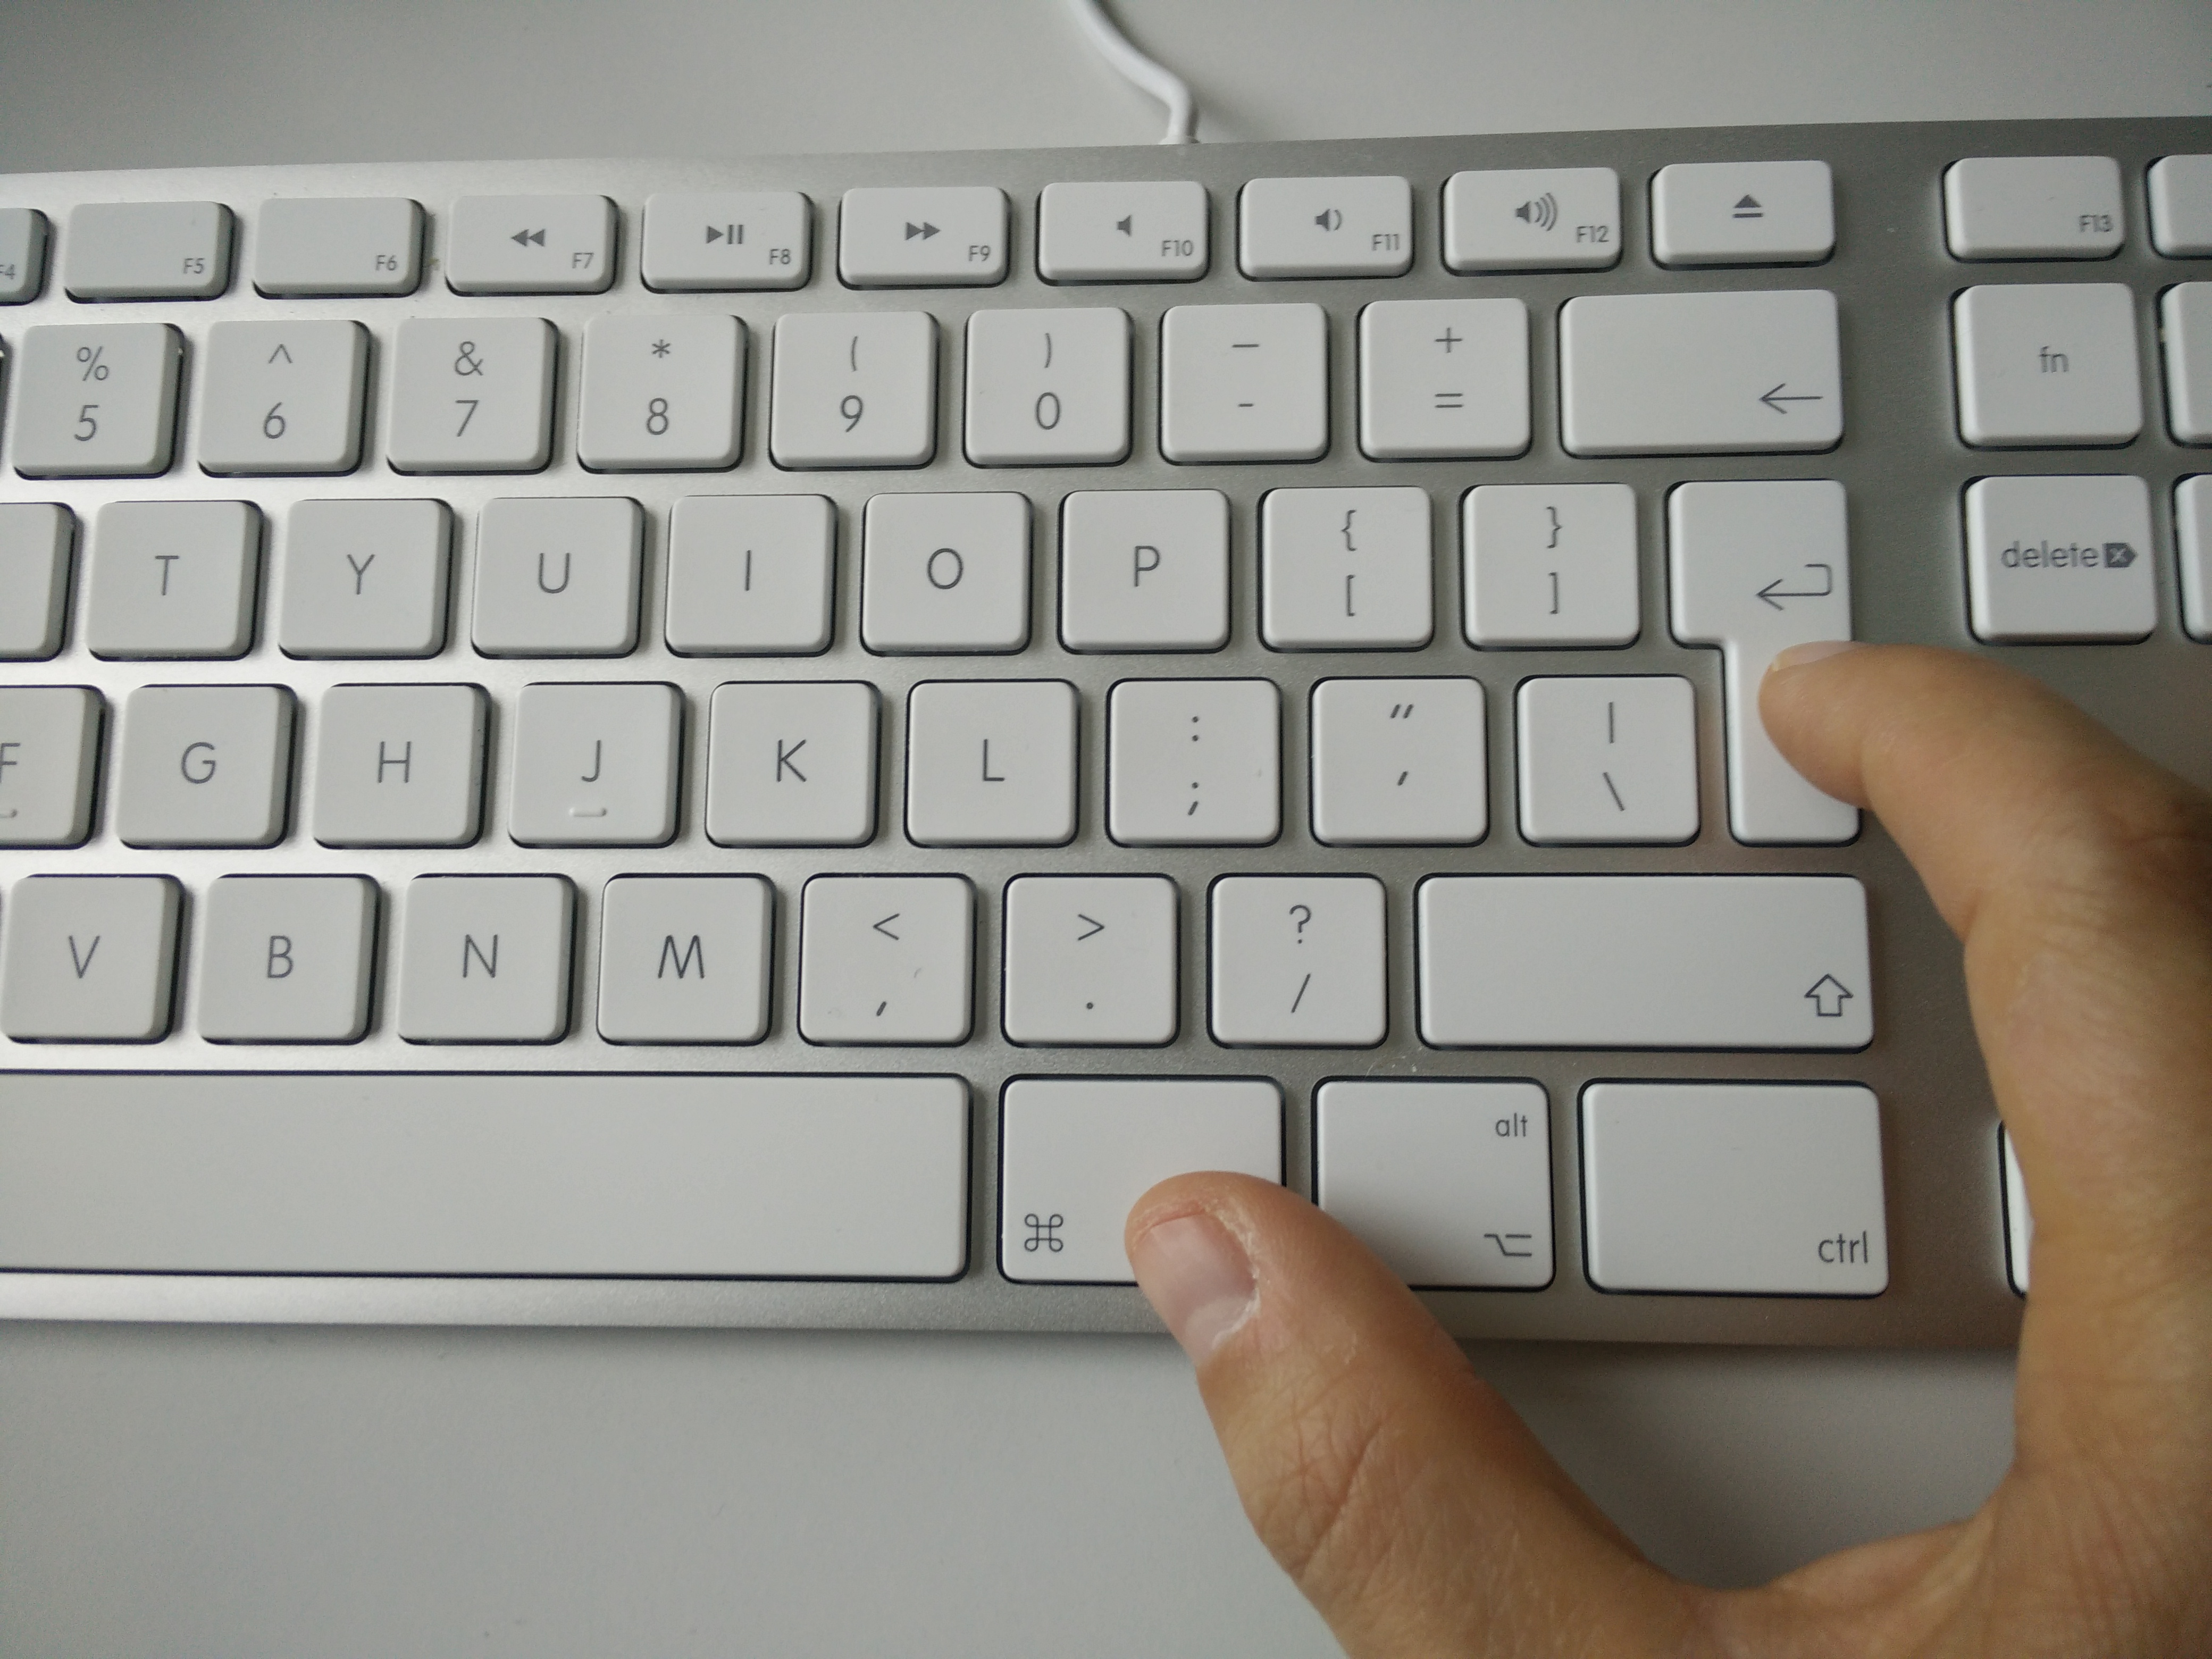
\includegraphics[width=400px]{images/commandreturn} 

}

\caption{Ah...the Command--Return shortcut (Control--Enter on PC) to send highlighted code from the Editor to the Console. Get used to this shortcut people. You're going to be using this a lot}\label{fig:commandreturn}
\end{figure}

99\% of the time, I use method 2, where I highlight the code I want,
then use the Command--Return shortcut . However, method 3 is great for
trouble-shooting code line-by-line.

\section{A brief style guide: Commenting and
spacing}\label{a-brief-style-guide-commenting-and-spacing}

Like all programming languages, R isn't just meant to be read by a
computer, it's also meant to be read by other humans -- or very
well-trained dolphins. For this reason, it's important that your code
looks nice and is understandable to other people and your future self.
To keep things brief, I won't provide a complete style guide -- instead
I'll focus on the two most critical aspects of good style: commenting
and spacing.

For a list of recommendations on how to make your code easier to follow,
check out Google's own company R Style guide at
\url{https://google-styleguide.googlecode.com/svn/trunk/Rguide.xml}

\begin{figure}

{\centering 
\includegraphics[width=400px]{images/futureself} 

}

\caption{As Stan discovered in season six of South Park, your future self is a lazy, possibly intoxicated moron. So do your future self a favor and make your code look nice. Also maybe go for a run once in a while.}\label{fig:futureself}
\end{figure}

\subsection{Commenting code with the \# (pound)
sign}\label{commenting-code-with-the-pound-sign}

Comments are completely ignored by R and are just there for whomever is
reading the code. You can use comments to explain what a certain line of
code is doing, or just to visually separate meaningful chunks of code
from each other. Comments in R are designated by a \# (pound) sign.
Whenever R encounters a \# sign, it will ignore \textbf{all} the code
after the \# sign on that line. Additionally, in most coding editors
(like RStudio) the editor will display comments in a separate color than
standard R code to remind you that it's a comment:

Here is an example of a short script that is nicely commented. Try to
make your scripts look like this!

\begin{Shaded}
\begin{Highlighting}[]
\CommentTok{# Author: Pirate Jack}
\CommentTok{# Title: My nicely commented R Script}
\CommentTok{# Date: None today :(}

\CommentTok{# Step 1: Load the yarrr package}
\KeywordTok{library}\NormalTok{(yarrr)}

\CommentTok{# Step 2: See the column names in the movies dataset}
\KeywordTok{names}\NormalTok{(movies)}

\CommentTok{# Step 3: Calculations}

\CommentTok{# What percent of movies are sequels?}
\KeywordTok{mean}\NormalTok{(movies$sequel, }\DataTypeTok{na.rm =} \NormalTok{T)}

\CommentTok{# How much did Pirate's of the Caribbean: On Strager Tides make?}
\NormalTok{movies$revenue.all[movies$name ==}\StringTok{ 'Pirates of the Caribbean: On Stranger Tides'}\NormalTok{]}
\end{Highlighting}
\end{Shaded}

I cannot stress enough how important it is to comment your code! Trust
me, even if you don't plan on sharing your code with anyone else, keep
in mind that your future self will be reading it in the future.

\subsection{Spacing}\label{spacing}

Howwouldyouliketoreadabookiftherewerenospacesbetweenwords?
I'mguessingyouwouldn't.
Soeverytimeyouwritecodewithoutproperspacing,rememberthissentence.

Commenting isn't the only way to make your code legible. It's important
to make appropriate use of spaces and line breaks. For example, I
include spaces between arithmetic operators (like =, + and -) and after
commas (which we'll get to later). For example, look at the following
code:

\begin{figure}

{\centering 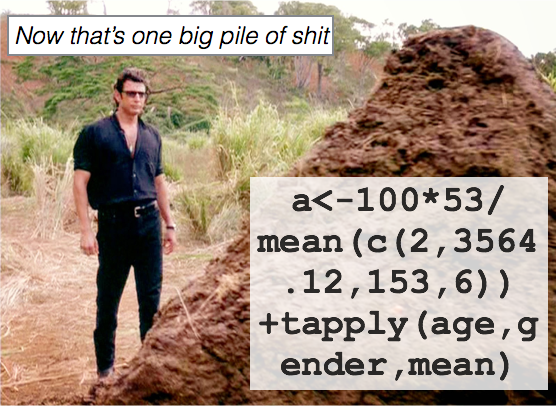
\includegraphics[width=400px]{images/pileofshit} 

}

\caption{Don't make your code look like what a sick Triceratops with diarrhea left behind for Jeff Goldblum.}\label{fig:pileofshit}
\end{figure}

\begin{Shaded}
\begin{Highlighting}[]
\CommentTok{# Shitty looking code}
\NormalTok{a<-(}\DecValTok{100+3}\NormalTok{)-}\DecValTok{2}
\KeywordTok{mean}\NormalTok{(}\KeywordTok{c}\NormalTok{(a/}\DecValTok{100}\NormalTok{,}\FloatTok{642564624.34}\NormalTok{))}
\KeywordTok{t.test}\NormalTok{(}\DataTypeTok{formula=}\NormalTok{revenue.all~sequel,}\DataTypeTok{data=}\NormalTok{movies)}
\KeywordTok{plot}\NormalTok{(}\DataTypeTok{x=}\NormalTok{movies$budget,}\DataTypeTok{y=}\NormalTok{movies$dvd.usa,}\DataTypeTok{main=}\StringTok{"myplot"}\NormalTok{)}
\end{Highlighting}
\end{Shaded}

That code looks like shit. Don't write code like that. It makes my eyes
hurt. Now, let's use some liberal amounts of commenting and spacing to
make it look less shitty.

\begin{Shaded}
\begin{Highlighting}[]
\CommentTok{# Some meaningless calculations. Not important}

\NormalTok{a <-}\StringTok{ }\NormalTok{(}\DecValTok{100} \NormalTok{+}\StringTok{ }\DecValTok{3}\NormalTok{) -}\StringTok{ }\DecValTok{2}
\KeywordTok{mean}\NormalTok{(}\KeywordTok{c}\NormalTok{(a /}\StringTok{ }\DecValTok{100}\NormalTok{, }\FloatTok{642564624.34}\NormalTok{))}

\CommentTok{# t.test comparing revenue of sequels v non-sequels}

\KeywordTok{t.test}\NormalTok{(}\DataTypeTok{formula =} \NormalTok{revenue.all ~}\StringTok{ }\NormalTok{sequel,}
       \DataTypeTok{data =} \NormalTok{movies)}

\CommentTok{# A scatterplot of budget and dvd revenue. }
\CommentTok{#  Hard to see a relationship}

\KeywordTok{plot}\NormalTok{(}\DataTypeTok{x =} \NormalTok{movies$budget,}
     \DataTypeTok{y =} \NormalTok{movies$dvd.usa,}
     \DataTypeTok{main =} \StringTok{"myplot"}\NormalTok{)}
\end{Highlighting}
\end{Shaded}

See how much better that second chunk of code looks? Not only do the
comments tell us the purpose behind the code, but there are spaces and
line-breaks separating distinct elements.

\section{Objects and functions}\label{objects-and-functions}

To understand how R works, you need to know that R revolves around two
things: objects and functions. Almost everything in R is either an
object or a function. In the following code chunk, I'll define a simple
object called \texttt{tattoos} using a function \texttt{c()}:

\begin{Shaded}
\begin{Highlighting}[]
\CommentTok{# 1: Create a vector object called tattoos}
\NormalTok{tattoos <-}\StringTok{ }\KeywordTok{c}\NormalTok{(}\DecValTok{4}\NormalTok{, }\DecValTok{67}\NormalTok{, }\DecValTok{23}\NormalTok{, }\DecValTok{4}\NormalTok{, }\DecValTok{10}\NormalTok{, }\DecValTok{35}\NormalTok{)}

\CommentTok{# 2: Apply the mean() function to the tattoos object}
\KeywordTok{mean}\NormalTok{(tattoos)}
\NormalTok{## [1] 24}
\end{Highlighting}
\end{Shaded}

What is an object? An object is a thing -- like a number, a dataset, a
summary statistic like a mean or standard deviation, or a statistical
test. Objects come in many different shapes and sizes in R. There are
simple objects like \textit{scalars} which represent single numbers,
\textbf{vectors} (like our \texttt{tattoos} object above) which
represent several numbers, more complex objects like \textbf{dataframes}
which represent tables of data, and even more complex objects like
\textbf{hypothesis tests} or \textbf{regression} which contain all sorts
of statistical information.

Different types of objects have different \emph{attributes}. For
example, a vector of data has a length attribute (i.e.; how many numbers
are in the vector), while a hypothesis test has many attributes such as
a test-statistic and a p-value. Don't worry if this is a bit confusing
now -- it will all become clearer when you meet these new objects in
person in later chapters. For now, just know that objects in R are
things, and different objects have different attributes.

What is a function? A function is a \emph{procedure} that typically
takes one or more objects as arguments (aka, inputs), does something
with those objects, then returns a new object. For example, the
\texttt{mean()} function we used above takes a vector object, like
\texttt{tattoos}, of numeric data as an argument, calculates the
arithmetic mean of those data, then returns a single number (a scalar)
as a result.A great thing about R is that you can easily create your own
functions that do whatever you want -- but we'll get to that much later
in the book. Thankfully, R has hundreds (thousands?) of built-in
functions that perform most of the basic analysis tasks you can think
of.

99\% of the time you are using R, you will do the following: 1) Define
objects. 2) Apply functions to those objects. 3) Repeat!. Seriously,
that's about it. However, as you'll soon learn, the hard part is knowing
how to define objects they way you want them, and knowing which
function(s) will accomplish the task you want for your objects.

\subsection{Numbers versus characters}\label{numbers-versus-characters}

For the most part, objects in R come in one of two flavors:
\textbf{numeric} and \textbf{character}. It is very important to keep
these two separate as certain functions, like \texttt{mean()}, and
\texttt{max()} will only work for numeric objects, while functions like
\texttt{grep()} and \texttt{strtrim()} only work for character objects.

A numeric object is just a number like \texttt{1}, \texttt{10} or
\texttt{3.14}. You don't have to do anything special to create a numeric
object, just type it like you were using a calculator.

\begin{Shaded}
\begin{Highlighting}[]
\CommentTok{# These are all numeric objects}
\DecValTok{1}
\DecValTok{10}
\FloatTok{3.14}
\end{Highlighting}
\end{Shaded}

A \textbf{character} object is a name like \texttt{"Madisen"},
\texttt{"Brian"}, or \texttt{"University\ of\ Konstanz"}. To specify a
character object, you need to include quotation marks \texttt{""} around
the text.

\begin{Shaded}
\begin{Highlighting}[]
\CommentTok{# These are all character objects}
\StringTok{"Madisen"}
\StringTok{"Brian"}
\StringTok{"10"}
\end{Highlighting}
\end{Shaded}

If you try to perform a function or operation meant for a numeric object
on a character object (and vice-versa), R will yell at you. For example,
here's what happens when I try to take the mean of the two character
objects \texttt{"1"} and \texttt{"10"}:

\begin{Shaded}
\begin{Highlighting}[]
\CommentTok{# This will return an error because the arguments are not numeric!}
\KeywordTok{mean}\NormalTok{(}\KeywordTok{c}\NormalTok{(}\StringTok{"1"}\NormalTok{, }\StringTok{"10"}\NormalTok{))}
\end{Highlighting}
\end{Shaded}

Warning message: argument is not numeric or logical, returning NA

If I make sure that the arguments are numeric (by not including the
quotation marks), I won't receive the error:

\begin{Shaded}
\begin{Highlighting}[]
\CommentTok{# This is ok!}
\KeywordTok{mean}\NormalTok{(}\KeywordTok{c}\NormalTok{(}\DecValTok{1}\NormalTok{, }\DecValTok{10}\NormalTok{))}
\NormalTok{## [1] 5.5}
\end{Highlighting}
\end{Shaded}

\subsection{Creating new objects with
\textless{}-}\label{creating-new-objects-with--}

By now you know that you can use R to do simple calculations. But to
really take advantage of R, you need to know how to create and
manipulate objects. All of the data, analyses, and even plots, you use
and create are, or can be, saved as objects in R. For example the
\texttt{movies} dataset which we've used before is an object stored in
the \texttt{yarrr} package. This object was defined in the
\texttt{yarrr} package with the name \texttt{movies}. When you loaded
the \texttt{yarrr} package with the
\texttt{library(\textquotesingle{}yarrr\textquotesingle{})} command, you
told R to give you access to the \texttt{movies} object. Once the object
was loaded, we could use it to calculate descriptive statistics,
hypothesis tests, and to create plots.

To create new objects in R, you need to do \emph{object assignment}.
Object assignment is our way of storing information, such as a number or
a statistical test, into something we can easily refer to later. This is
a pretty big deal. Object assignment allows us to store data objects
under relevant names which we can then use to slice and dice specific
data objects anytime we'd like to.

To do an assignment, we use the almighty \texttt{\textless{}-} operator
called \emph{assign} To assign something to a new object (or to change
an existing object), use the notation
\texttt{object\ \textless{}-\ ...}\}, where \texttt{object} is the new
(or updated) object, and \texttt{...} is whatever you want to store in
\texttt{object}. Let's start by creating a very simple object called
\texttt{a} and assigning the value of 100 to it:

\marginnote{Good object names strike a balance between being easy to type (i.e.; short names) and interpret. If you have several datasets, it's probably not a good idea to name them \texttt{a}, \texttt{b}, \texttt{c} because you'll forget which is which. However, using long names like \texttt{March2015Group1OnlyFemales} will give you carpel tunnel syndrome.}

\begin{Shaded}
\begin{Highlighting}[]
\CommentTok{# Create a new object called a with a value of 100}
\NormalTok{a <-}\StringTok{ }\DecValTok{100}
\end{Highlighting}
\end{Shaded}

Once you run this code, you'll notice that R doesn't tell you anything.
However, as long as you didn't type something wrong, R should now have a
new object called \texttt{a} which contains the number 100. If you want
to see the value, you need to call the object by just executing its
name. This will print the value of the object to the console:

\begin{Shaded}
\begin{Highlighting}[]
\CommentTok{# Print the object a}
\NormalTok{a}
\NormalTok{## [1] 100}
\end{Highlighting}
\end{Shaded}

Now, R will print the value of \texttt{a} (in this case 100) to the
console. If you try to evaluate an object that is not yet defined, R
will return an error. For example, let's try to print the object
\texttt{b} which we haven't yet defined:

\begin{Shaded}
\begin{Highlighting}[]
\NormalTok{b}
\end{Highlighting}
\end{Shaded}

Error: object `b' not found

As you can see, R yelled at us because the object \texttt{b} hasn't been
defined yet.

Once you've defined an object, you can combine it with other objects
using basic arithmetic. Let's create objects \texttt{a} and \texttt{b}
and play around with them.

\begin{Shaded}
\begin{Highlighting}[]
\NormalTok{a <-}\StringTok{ }\DecValTok{1}
\NormalTok{b <-}\StringTok{ }\DecValTok{100}

\CommentTok{# What is a + b?}
\NormalTok{a +}\StringTok{ }\NormalTok{b}
\NormalTok{## [1] 101}

\CommentTok{# Assign a + b to a new object (c)}
\NormalTok{c <-}\StringTok{ }\NormalTok{a +}\StringTok{ }\NormalTok{b}

\CommentTok{# What is c?}
\NormalTok{c}
\NormalTok{## [1] 101}
\end{Highlighting}
\end{Shaded}

\subsubsection{To change an object, you must assign it
again!}\label{to-change-an-object-you-must-assign-it-again}

Normally I try to avoid excessive emphasis, but because this next
sentence is so important, I have to just go for it. Here it goes\ldots{}

\textbf{To change an object, you \textit{must} assign it again!}

No matter what you do with an object, if you don't assign it again, it
won't change. For example, let's say you have an object \texttt{z} with
a value of 0. You'd like to add 1 to \texttt{z} in order to make it 1.
To do this, you might want to just enter \texttt{z\ +\ 1} -- but that
won't do the job. Here's what happens if you \textbf{don't} assign it
again:

\begin{Shaded}
\begin{Highlighting}[]
\NormalTok{z <-}\StringTok{ }\DecValTok{0}
\NormalTok{z +}\StringTok{ }\DecValTok{1}
\NormalTok{## [1] 1}
\end{Highlighting}
\end{Shaded}

Ok! Now let's see the value of \texttt{z}

\begin{Shaded}
\begin{Highlighting}[]
\NormalTok{z}
\NormalTok{## [1] 0}
\end{Highlighting}
\end{Shaded}

Damn! As you can see, the value of z is still 0! What went wrong? Oh
yeah\ldots{}

\textbf{To change an object, you \emph{must} assign it again!}

The problem is that when we wrote \texttt{z\ +\ 1} on the second line, R
thought we just wanted it to calculate and print the value of
\texttt{z\ +\ 1}, without storing the result as a new \texttt{z} object.
If we want to actually update the value of \texttt{z}, we need to
reassign the result back to \texttt{z} as follows:

\begin{Shaded}
\begin{Highlighting}[]
\NormalTok{z <-}\StringTok{ }\DecValTok{0}
\NormalTok{z <-}\StringTok{ }\NormalTok{z +}\StringTok{ }\DecValTok{1}  \CommentTok{# Now I'm REALLY changing z}
\NormalTok{z}
\NormalTok{## [1] 1}
\end{Highlighting}
\end{Shaded}

Phew, z is now 1. Because we used assignment, z has been updated. About
freaking time.

\subsection{How to name objects}\label{how-to-name-objects}

You can create object names using any combination of letters and a few
special characters (like \texttt{.} and \texttt{\_}). Here are some
valid object names

\begin{Shaded}
\begin{Highlighting}[]
\CommentTok{# Valid object names}
\NormalTok{group.mean <-}\StringTok{ }\FloatTok{10.21}
\NormalTok{my.age <-}\StringTok{ }\DecValTok{32}
\NormalTok{FavoritePirate <-}\StringTok{ "Jack Sparrow"}
\NormalTok{sum}\FloatTok{.1}\NormalTok{.to}\FloatTok{.5} \NormalTok{<-}\StringTok{ }\DecValTok{1} \NormalTok{+}\StringTok{ }\DecValTok{2} \NormalTok{+}\StringTok{ }\DecValTok{3} \NormalTok{+}\StringTok{ }\DecValTok{4} \NormalTok{+}\StringTok{ }\DecValTok{5}
\end{Highlighting}
\end{Shaded}

All the object names above are perfectly valid. Now, let's look at some
examples of \emph{invalid} object names. These object names are all
invalid because they either contain spaces, start with numbers, or have
invalid characters:

\begin{Shaded}
\begin{Highlighting}[]
\CommentTok{# Invalid object names!}
\NormalTok{famale ages <-}\StringTok{ }\DecValTok{50} \CommentTok{# spaces}
\NormalTok{5experiment <-}\StringTok{ }\DecValTok{50} \CommentTok{# starts with a number}
\NormalTok{a!}\StringTok{ }\ErrorTok{<}\NormalTok{-}\StringTok{ }\DecValTok{50} \CommentTok{# has an invalid character}
\end{Highlighting}
\end{Shaded}

If you try running the code above in R, you will receive a warning
message starting with

Error: unexpected symbol

. Anytime you see this warning in R, it almost always means that you
have a naming error of some kind.

\subsubsection{R is case-sensitive!}\label{r-is-case-sensitive}

\begin{figure}

{\centering 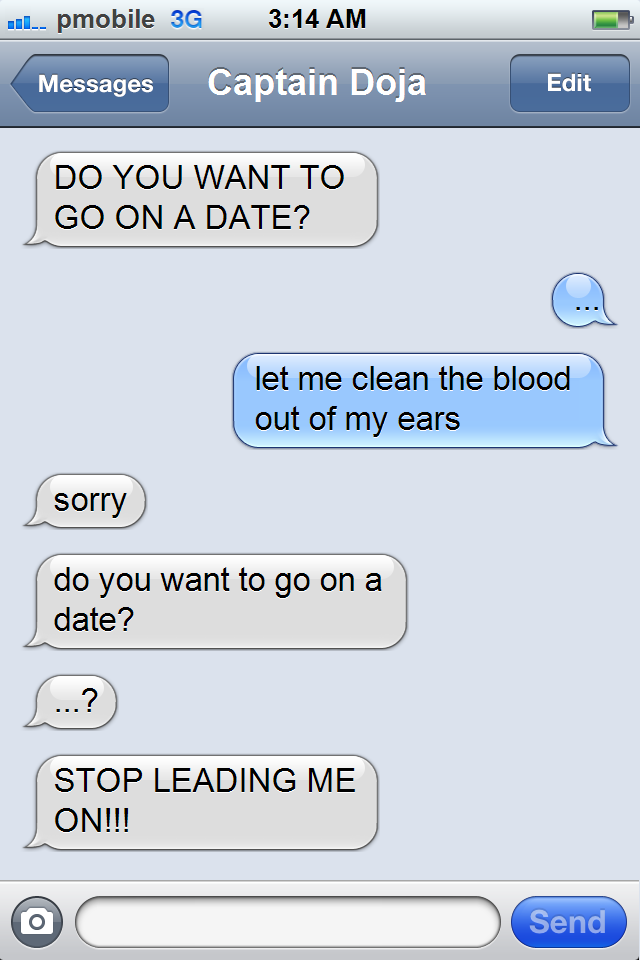
\includegraphics[width=300px]{images/datetext} 

}

\caption{Like a text message, you should probably watch your use of capitalization in R.}\label{fig:datetext}
\end{figure}

Like English, R is case-sensitive -- it R treats capital letters
differently from lower-case letters. For example, the four following
objects \texttt{Plunder}, \texttt{plunder} and \texttt{PLUNDER} are
totally different objects in R:

\begin{Shaded}
\begin{Highlighting}[]
\CommentTok{# These are all different objects}
\NormalTok{Plunder <-}\StringTok{ }\DecValTok{1}
\NormalTok{plunder <-}\StringTok{ }\DecValTok{100}
\NormalTok{PLUNDER <-}\StringTok{ }\DecValTok{5}
\end{Highlighting}
\end{Shaded}

I try to avoid using too many capital letters in object names because
they require me to hold the shift key. This may sound silly, but you'd
be surprised how much easier it is to type \texttt{mydata} than
\texttt{MyData} 100 times.

\subsection{Example: Pirates of The
Caribbean}\label{example-pirates-of-the-caribbean}

Let's do a more practical example -- we'll define an object called
\texttt{blackpearl.usd} which has the global revenue of Pirates of the
Caribbean: Curse of the Black Pearl in U.S. dollars. A quick Google
search showed me that the revenue was \$634,954,103. I'll create the new
object using assignment:

\begin{Shaded}
\begin{Highlighting}[]
\NormalTok{blackpearl.usd <-}\StringTok{ }\DecValTok{634954103}
\end{Highlighting}
\end{Shaded}

Now, my fellow European pirates might want to know how much this is in
Euros. Let's create a new object called \texttt{\{blackpearl.eur} which
converts our original value to Euros by multiplying the original amount
by 0.88 (assuming 1 USD = 0.88 EUR)

\begin{Shaded}
\begin{Highlighting}[]
\NormalTok{blackpearl.eur <-}\StringTok{ }\NormalTok{blackpearl.usd *}\StringTok{ }\FloatTok{0.88}
\NormalTok{blackpearl.eur}
\NormalTok{## [1] 5.6e+08}
\end{Highlighting}
\end{Shaded}

It looks like the movie made 558,759,611 in Euros. Not bad. Now, let's
see how much more Pirates of the Caribbean 2: Dead Man's Chest made
compared to ``Curse of the Black Pearl.'' Another Google search
uncovered that Dead Man's Chest made \$1,066,215,812 (that wasn't a
mistype, the freaking movie made over a billion dollars).

\begin{Shaded}
\begin{Highlighting}[]
\NormalTok{deadman.usd <-}\StringTok{ }\DecValTok{1066215812}
\end{Highlighting}
\end{Shaded}

Now, I'll divide \texttt{deadman.usd} by \texttt{blackpearl.usd}:

\begin{Shaded}
\begin{Highlighting}[]
\NormalTok{deadman.usd /}\StringTok{ }\NormalTok{blackpearl.usd}
\NormalTok{## [1] 1.7}
\end{Highlighting}
\end{Shaded}

It looks like ``Dead Man's Chest'' made 168\% as much as ``Curse of the
Black Pearl'' - not bad for two movies based off of a ride from
Disneyland.

\section{Test your R might!}\label{test-your-r-might}

\begin{enumerate}
\def\labelenumi{\arabic{enumi}.}
\item
  Create a new R script. Using comments, write your name, the date, and
  `'Testing my Chapter 2 R Might'' at the top of the script. Write your
  answers to the rest of these exercises on this script, and be sure to
  copy and paste the original questions using comments! Your script
  should \textit{only} contain valid R code and comments.
\item
  Which (if any) of the following objects names is/are invalid?
\end{enumerate}

\begin{Shaded}
\begin{Highlighting}[]
\NormalTok{thisone <-}\StringTok{ }\DecValTok{1}
\NormalTok{THISONE <-}\StringTok{ }\DecValTok{2}
\NormalTok{1This <-}\StringTok{ }\DecValTok{3}
\NormalTok{this.one <-}\StringTok{ }\DecValTok{4}
\NormalTok{This}\FloatTok{.1} \NormalTok{<-}\StringTok{ }\DecValTok{5}
\NormalTok{ThIS.....ON...E <-}\StringTok{ }\DecValTok{6}
\NormalTok{This!On!e <-}\StringTok{ }\DecValTok{7}
\NormalTok{lkjasdfkjsdf <-}\StringTok{ }\DecValTok{8}
\end{Highlighting}
\end{Shaded}

\begin{enumerate}
\def\labelenumi{\arabic{enumi}.}
\setcounter{enumi}{2}
\item
  2015 was a good year for pirate booty - your ship collected 100,800
  gold coins. Create an object called \texttt{gold.in.2015} and assign
  the correct value to it.
\item
  Oops, during the last inspection we discovered that one of your
  pirates Skippy McGee hid 800 gold coins in his underwear. Go ahead and
  add those gold coins to the object \texttt{gold.in.2015}. Next, create
  an object called \texttt{plank.list} with the name of the pirate
  thief.
\item
  Look at the code below. What will R return after the third line? Make
  a prediction, then test the code yourself.
\end{enumerate}

\begin{Shaded}
\begin{Highlighting}[]
\NormalTok{a <-}\StringTok{ }\DecValTok{10}
\NormalTok{a +}\StringTok{ }\DecValTok{10}
\NormalTok{a}
\end{Highlighting}
\end{Shaded}

\chapter{Scalers and vectors}\label{scalersvectors}

\begin{figure}

{\centering 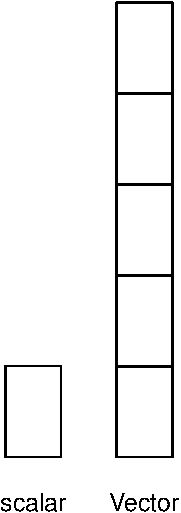
\includegraphics{YaRrr_files/figure-latex/scalervector-1} 

}

\caption{Visual depiction of a scalar and vector. Deep shit. Wait until we get to matrices - you're going to lose it.}\label{fig:scalervector}
\end{figure}

\begin{Shaded}
\begin{Highlighting}[]
\CommentTok{# Crew information}
\NormalTok{captain.name <-}\StringTok{ "Jack"}
\NormalTok{captain.age <-}\StringTok{ }\DecValTok{33}

\NormalTok{crew.names <-}\StringTok{ }\KeywordTok{c}\NormalTok{(}\StringTok{"Heath"}\NormalTok{, }\StringTok{"Vincent"}\NormalTok{, }\StringTok{"Maya"}\NormalTok{, }\StringTok{"Becki"}\NormalTok{)}
\NormalTok{crew.ages <-}\StringTok{ }\KeywordTok{c}\NormalTok{(}\DecValTok{19}\NormalTok{, }\DecValTok{35}\NormalTok{, }\DecValTok{22}\NormalTok{, }\DecValTok{44}\NormalTok{)}
\NormalTok{crew.sex <-}\StringTok{ }\KeywordTok{c}\NormalTok{(}\KeywordTok{rep}\NormalTok{(}\StringTok{"M"}\NormalTok{, }\DataTypeTok{times =} \DecValTok{2}\NormalTok{), }\KeywordTok{rep}\NormalTok{(}\StringTok{"F"}\NormalTok{, }\DataTypeTok{times =} \DecValTok{2}\NormalTok{))}
\NormalTok{crew.ages.decade <-}\StringTok{ }\NormalTok{crew.ages /}\StringTok{ }\DecValTok{10}

\CommentTok{# Earnings over first 10 days at sea}
\NormalTok{days <-}\StringTok{ }\DecValTok{1}\NormalTok{:}\DecValTok{10}
\NormalTok{gold <-}\StringTok{ }\KeywordTok{seq}\NormalTok{(}\DataTypeTok{from =} \DecValTok{10}\NormalTok{, }\DataTypeTok{to =} \DecValTok{100}\NormalTok{, }\DataTypeTok{by =} \DecValTok{10}\NormalTok{)}
\NormalTok{silver <-}\StringTok{ }\KeywordTok{rep}\NormalTok{(}\DecValTok{50}\NormalTok{, }\DataTypeTok{times =} \DecValTok{10}\NormalTok{)}
\NormalTok{total <-}\StringTok{ }\NormalTok{gold +}\StringTok{ }\NormalTok{silver}
\end{Highlighting}
\end{Shaded}

People are not objects. But R is full of them. Here are some of the
basic ones.

\section{Scalars}\label{scalars}

The simplest object type in R is a \textbf{scalar}. A scalar object is
just a single value like a number or a name. In the previous chapter we
defined several scalar objects. Here are examples of numeric scalars:

\begin{Shaded}
\begin{Highlighting}[]
\CommentTok{# Examples of numeric scalers}
\NormalTok{a <-}\StringTok{ }\DecValTok{100}
\NormalTok{b <-}\StringTok{ }\DecValTok{3} \NormalTok{/}\StringTok{ }\DecValTok{100}
\NormalTok{c <-}\StringTok{ }\NormalTok{(a +}\StringTok{ }\NormalTok{b) /}\StringTok{ }\NormalTok{b}
\end{Highlighting}
\end{Shaded}

Scalars don't have to be numeric, they can also be \textbf{characters}
(also known as strings). In R, you denote characters using quotation
marks. Here are examples of character scalars:

\begin{Shaded}
\begin{Highlighting}[]
\CommentTok{# Examples of character scalers}
\NormalTok{d <-}\StringTok{ "ship"}
\NormalTok{e <-}\StringTok{ "cannon"}
\NormalTok{f <-}\StringTok{ "Do any modern armies still use cannons?"}
\end{Highlighting}
\end{Shaded}

As you can imagine, R treats numeric and character scalars differently.
For example, while you can do basic arithmetic operations on numeric
scalars -- they won't work on character scalars. If you try to perform
numeric operations (like addition) on character scalars, you'll get an
error like this one:

\begin{Shaded}
\begin{Highlighting}[]
\NormalTok{a <-}\StringTok{ "1"}
\NormalTok{b <-}\StringTok{ "2"}
\NormalTok{a +}\StringTok{ }\NormalTok{b}
\end{Highlighting}
\end{Shaded}

Error in a + b: non-numeric argument to binary operator

If you see an error like this one, it means that you're trying to apply
numeric operations to character objects. That's just sick and wrong.

\section{Vectors}\label{vectors}

Now let's move onto \texttt{vectors}. A vector object is just a
combination of several scalars stored as a single object. For example,
the numbers from one to ten could be a vector of length 10, and the
characters in the English alphabet could be a vector of length 26. Like
scalars, vectors can be either numeric or character (but not both!).

There are many ways to create vectors in R. Here are the methods we will
cover in this chapter:

\begin{longtable}[]{@{}lll@{}}
\caption{Functions to create vectors.}\tabularnewline
\toprule
\begin{minipage}[b]{0.34\columnwidth}\raggedright\strut
Function\strut
\end{minipage} & \begin{minipage}[b]{0.39\columnwidth}\raggedright\strut
Example\strut
\end{minipage} & \begin{minipage}[b]{0.15\columnwidth}\raggedright\strut
Result\strut
\end{minipage}\tabularnewline
\midrule
\endfirsthead
\toprule
\begin{minipage}[b]{0.34\columnwidth}\raggedright\strut
Function\strut
\end{minipage} & \begin{minipage}[b]{0.39\columnwidth}\raggedright\strut
Example\strut
\end{minipage} & \begin{minipage}[b]{0.15\columnwidth}\raggedright\strut
Result\strut
\end{minipage}\tabularnewline
\midrule
\endhead
\begin{minipage}[t]{0.34\columnwidth}\raggedright\strut
\texttt{c(a,\ b,\ ...)}\strut
\end{minipage} & \begin{minipage}[t]{0.39\columnwidth}\raggedright\strut
\texttt{c(1,\ 5,\ 9)}\strut
\end{minipage} & \begin{minipage}[t]{0.15\columnwidth}\raggedright\strut
1, 5, 9\strut
\end{minipage}\tabularnewline
\begin{minipage}[t]{0.34\columnwidth}\raggedright\strut
\texttt{a:b}\strut
\end{minipage} & \begin{minipage}[t]{0.39\columnwidth}\raggedright\strut
\texttt{1:5}\strut
\end{minipage} & \begin{minipage}[t]{0.15\columnwidth}\raggedright\strut
1, 2, 3, 4, 5\strut
\end{minipage}\tabularnewline
\begin{minipage}[t]{0.34\columnwidth}\raggedright\strut
\texttt{seq(from,\ to,\ by,\ length.out)}\strut
\end{minipage} & \begin{minipage}[t]{0.39\columnwidth}\raggedright\strut
\texttt{seq(from\ =\ 0,\ to\ =\ 6,\ by\ =\ 2)}\strut
\end{minipage} & \begin{minipage}[t]{0.15\columnwidth}\raggedright\strut
0, 2, 4, 6\strut
\end{minipage}\tabularnewline
\begin{minipage}[t]{0.34\columnwidth}\raggedright\strut
\texttt{rep(x,\ times,\ each,\ length.out)}\strut
\end{minipage} & \begin{minipage}[t]{0.39\columnwidth}\raggedright\strut
\texttt{rep(c(7,\ 8),\ times\ =\ 2,\ each\ =\ 2)}\strut
\end{minipage} & \begin{minipage}[t]{0.15\columnwidth}\raggedright\strut
7, 7, 8, 8, 7, 7, 8, 8\strut
\end{minipage}\tabularnewline
\bottomrule
\end{longtable}

The simplest way to create a vector is with the \texttt{c()} function.
The c here stands for concatenate, which means ``bring them together''.
The \texttt{c()} function takes several scalars as arguments, and
returns a vector containing those objects. When using c(), place a comma
in between the objects (scalars or vectors) you want to combine:

Let's use the \texttt{c()} function to create a vector called \texttt{a}
containing the integers from 1 to 5.

\begin{Shaded}
\begin{Highlighting}[]
\CommentTok{# Create an object a with the integers from 1 to 5}
\NormalTok{a <-}\StringTok{ }\KeywordTok{c}\NormalTok{(}\DecValTok{1}\NormalTok{, }\DecValTok{2}\NormalTok{, }\DecValTok{3}\NormalTok{, }\DecValTok{4}\NormalTok{, }\DecValTok{5}\NormalTok{)}

\CommentTok{# Print the result}
\NormalTok{a}
\NormalTok{## [1] 1 2 3 4 5}
\end{Highlighting}
\end{Shaded}

As you can see, R has stored all 5 numbers in the object \texttt{a}.
Thanks R!

You can also create longer vectors by combining vectors you have already
defined. Let's create a vector of the numbers from 1 to 10 by first
generating a vector \texttt{a} from 1 to 5, and a vector \texttt{b} from
6 to 10 then combine them into a single vector \texttt{x}:

\begin{Shaded}
\begin{Highlighting}[]
\NormalTok{a <-}\StringTok{ }\KeywordTok{c}\NormalTok{(}\DecValTok{1}\NormalTok{, }\DecValTok{2}\NormalTok{, }\DecValTok{3}\NormalTok{, }\DecValTok{4}\NormalTok{, }\DecValTok{5}\NormalTok{)}
\NormalTok{b <-}\StringTok{ }\KeywordTok{c}\NormalTok{(}\DecValTok{6}\NormalTok{, }\DecValTok{7}\NormalTok{, }\DecValTok{8}\NormalTok{, }\DecValTok{9}\NormalTok{, }\DecValTok{10}\NormalTok{)}
\NormalTok{x <-}\StringTok{ }\KeywordTok{c}\NormalTok{(a, b)}
\NormalTok{x}
\NormalTok{##  [1]  1  2  3  4  5  6  7  8  9 10}
\end{Highlighting}
\end{Shaded}

You can also create character vectors by using the \texttt{c()} function
to combine character scalars into character vectors:

\begin{figure}

{\centering 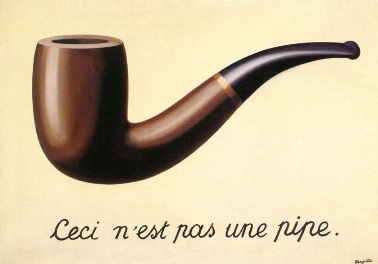
\includegraphics[width=400px]{images/magrittepipe} 

}

\caption{This is not a pipe. It is a character vector.}\label{fig:unnamed-chunk-70}
\end{figure}

\begin{Shaded}
\begin{Highlighting}[]
\NormalTok{char.vec <-}\StringTok{ }\KeywordTok{c}\NormalTok{(}\StringTok{"Leci"}\NormalTok{, }\StringTok{"nest"}\NormalTok{, }\StringTok{"pas"}\NormalTok{, }\StringTok{"une"}\NormalTok{, }\StringTok{"pipe"}\NormalTok{)}
\NormalTok{char.vec}
\NormalTok{## [1] "Leci" "nest" "pas"  "une"  "pipe"}
\end{Highlighting}
\end{Shaded}

While the \texttt{c()} function is the most straightforward way to
create a vector, it's also one of the most tedious. For example, let's
say you wanted to create a vector of all integers from 1 to 100. You
definitely don't want to have to type all the numbers into a c()
operator. Thankfully, R has many simple built-in functions for
generating numeric vectors. Let's start with three of them:
\texttt{a:b}, \texttt{seq()}, and \texttt{rep()}:

\subsection{a:b}\label{ab}

The \texttt{a:b} function takes two numeric scalars \texttt{a} and
\texttt{b} as arguments, and returns a vector of numbers from the
starting point \texttt{a} to the ending point \texttt{b} in steps of 1.

Here are some examples of the \texttt{a:b} function in action. As you'll
see, you can go backwards or forwards, or make sequences between
non-integers:

\begin{Shaded}
\begin{Highlighting}[]
\DecValTok{1}\NormalTok{:}\DecValTok{10}
\NormalTok{##  [1]  1  2  3  4  5  6  7  8  9 10}
\DecValTok{10}\NormalTok{:}\DecValTok{1}
\NormalTok{##  [1] 10  9  8  7  6  5  4  3  2  1}
\FloatTok{2.5}\NormalTok{:}\FloatTok{8.5}
\NormalTok{## [1] 2.5 3.5 4.5 5.5 6.5 7.5 8.5}
\end{Highlighting}
\end{Shaded}

\subsection{seq()}\label{seq}

\begin{longtable}[]{@{}ll@{}}
\toprule
\begin{minipage}[b]{0.35\columnwidth}\raggedright\strut
Argument\strut
\end{minipage} & \begin{minipage}[b]{0.41\columnwidth}\raggedright\strut
Definition\strut
\end{minipage}\tabularnewline
\midrule
\endhead
\begin{minipage}[t]{0.35\columnwidth}\raggedright\strut
\texttt{from}\strut
\end{minipage} & \begin{minipage}[t]{0.41\columnwidth}\raggedright\strut
The start of the sequence\strut
\end{minipage}\tabularnewline
\begin{minipage}[t]{0.35\columnwidth}\raggedright\strut
\texttt{to}\strut
\end{minipage} & \begin{minipage}[t]{0.41\columnwidth}\raggedright\strut
The end of the sequence\strut
\end{minipage}\tabularnewline
\begin{minipage}[t]{0.35\columnwidth}\raggedright\strut
\texttt{by}\strut
\end{minipage} & \begin{minipage}[t]{0.41\columnwidth}\raggedright\strut
The step-size of the sequence\strut
\end{minipage}\tabularnewline
\begin{minipage}[t]{0.35\columnwidth}\raggedright\strut
\texttt{length.out}\strut
\end{minipage} & \begin{minipage}[t]{0.41\columnwidth}\raggedright\strut
The desired length of the final sequence (only use if you don't specify
\texttt{by})\strut
\end{minipage}\tabularnewline
\bottomrule
\end{longtable}

The \texttt{seq()} function is a more flexible version of \texttt{a:b}.
Like \texttt{a:b}, \texttt{seq()} allows you to create a sequence from a
starting number to an ending number. However, \texttt{seq()\}}, has
additional arguments that allow you to specify either the size of the
steps between numbers, or the total length of the sequence:

The \texttt{seq()} function has two new arguments \texttt{by} and
\texttt{length.out}. If you use the \texttt{by} argument, the sequence
will be in steps of the input to the \texttt{by} argument:

\begin{Shaded}
\begin{Highlighting}[]
\CommentTok{# Create the numbers from 1 to 10 in steps of 1}
\KeywordTok{seq}\NormalTok{(}\DataTypeTok{from =} \DecValTok{1}\NormalTok{, }\DataTypeTok{to =} \DecValTok{10}\NormalTok{, }\DataTypeTok{by =} \DecValTok{1}\NormalTok{)}
\NormalTok{##  [1]  1  2  3  4  5  6  7  8  9 10}

\CommentTok{# Integers from 0 to 100 in steps of 10}
\KeywordTok{seq}\NormalTok{(}\DataTypeTok{from =} \DecValTok{0}\NormalTok{, }\DataTypeTok{to =} \DecValTok{100}\NormalTok{, }\DataTypeTok{by =} \DecValTok{10}\NormalTok{)}
\NormalTok{##  [1]   0  10  20  30  40  50  60  70  80  90 100}
\end{Highlighting}
\end{Shaded}

If you use the \texttt{length.out} argument, the sequence will have
length equal to \texttt{length.out}.

\begin{Shaded}
\begin{Highlighting}[]
\CommentTok{# Create 10 numbers from 1 to 5}
\KeywordTok{seq}\NormalTok{(}\DataTypeTok{from =} \DecValTok{1}\NormalTok{, }\DataTypeTok{to =} \DecValTok{5}\NormalTok{, }\DataTypeTok{length.out =} \DecValTok{10}\NormalTok{)}
\NormalTok{##  [1] 1.0 1.4 1.9 2.3 2.8 3.2 3.7 4.1 4.6 5.0}

\CommentTok{# 3 numbers from 0 to 100}
\KeywordTok{seq}\NormalTok{(}\DataTypeTok{from =} \DecValTok{0}\NormalTok{, }\DataTypeTok{to =} \DecValTok{100}\NormalTok{, }\DataTypeTok{length.out =} \DecValTok{3}\NormalTok{)}
\NormalTok{## [1]   0  50 100}
\end{Highlighting}
\end{Shaded}

\subsection{rep()}\label{rep}

\begin{longtable}[]{@{}ll@{}}
\toprule
Argument & Definition\tabularnewline
\midrule
\endhead
\texttt{x} & A scalar or vector of values to repeat\tabularnewline
\texttt{times} & The number of times to repeat x\tabularnewline
\texttt{each} & The number of times to repeat each value within
x\tabularnewline
\texttt{length.out} & The desired length of the final
sequence\tabularnewline
\bottomrule
\end{longtable}

\begin{figure}

{\centering 
\includegraphics[width=400px]{images/rep} 

}

\caption{Not a good depiction of a rep in R.}\label{fig:rep}
\end{figure}

The \texttt{rep()} function allows you to repeat a scalar (or vector) a
specified number of times, or to a desired length. Let's do some reps.

\begin{Shaded}
\begin{Highlighting}[]
\KeywordTok{rep}\NormalTok{(}\DataTypeTok{x =} \DecValTok{3}\NormalTok{, }\DataTypeTok{times =} \DecValTok{10}\NormalTok{)}
\NormalTok{##  [1] 3 3 3 3 3 3 3 3 3 3}
\KeywordTok{rep}\NormalTok{(}\DataTypeTok{x =} \KeywordTok{c}\NormalTok{(}\DecValTok{1}\NormalTok{, }\DecValTok{2}\NormalTok{), }\DataTypeTok{each =} \DecValTok{3}\NormalTok{)}
\NormalTok{## [1] 1 1 1 2 2 2}
\KeywordTok{rep}\NormalTok{(}\DataTypeTok{x =} \DecValTok{1}\NormalTok{:}\DecValTok{3}\NormalTok{, }\DataTypeTok{length.out =} \DecValTok{10}\NormalTok{)}
\NormalTok{##  [1] 1 2 3 1 2 3 1 2 3 1}
\end{Highlighting}
\end{Shaded}

As you can see, you can can include an \texttt{a:b} call within a
\texttt{rep()}!

You can even combine the \texttt{times} and \texttt{each} arguments
within a single \texttt{rep()} function. For example, here's how to
create the sequence \{1, 1, 2, 2, 3, 3, 1, 1, 2, 2, 3, 3\} with one call
to \texttt{rep()}:

\begin{Shaded}
\begin{Highlighting}[]
\KeywordTok{rep}\NormalTok{(}\DataTypeTok{x =} \DecValTok{1}\NormalTok{:}\DecValTok{3}\NormalTok{, }\DataTypeTok{each =} \DecValTok{2}\NormalTok{, }\DataTypeTok{times =} \DecValTok{2}\NormalTok{)}
\NormalTok{##  [1] 1 1 2 2 3 3 1 1 2 2 3 3}
\end{Highlighting}
\end{Shaded}

\textbf{Warning! Vectors contain either numbers or characters, not both}

A vector can only contain one type of scalar: either numeric or
character. If you try to create a vector with numeric and character
scalars, then R will convert \emph{all} of the numeric scalars to
characters. In the next code chunk, I'll create a new vector called
\texttt{my.vec} that contains a mixture of numeric and character
scalars.

\begin{Shaded}
\begin{Highlighting}[]
\NormalTok{my.vec <-}\StringTok{ }\KeywordTok{c}\NormalTok{(}\StringTok{"a"}\NormalTok{, }\DecValTok{1}\NormalTok{, }\StringTok{"b"}\NormalTok{, }\DecValTok{2}\NormalTok{, }\StringTok{"c"}\NormalTok{, }\DecValTok{3}\NormalTok{)}
\NormalTok{my.vec}
\NormalTok{## [1] "a" "1" "b" "2" "c" "3"}
\end{Highlighting}
\end{Shaded}

As you can see from the output, \texttt{my.vec} is stored as a character
vector where all the numbers are converted to characters.

\section{Generating random data}\label{generating-random-data}

Because R is a language built for statistics, it contains many functions
that allow you generate random data -- either from a vector of data that
you specify (like Heads or Tails from a coin), or from an established
\emph{probability distribution}, like the Normal or Uniform
distribution.

In the next section we'll go over the standard \texttt{sample()}
function for drawing random values from a vector. We'll then cover some
of the most commonly used probability distributions: Normal and Uniform.

\subsection{sample()}\label{sample}

\begin{longtable}[]{@{}ll@{}}
\toprule
\begin{minipage}[b]{0.14\columnwidth}\raggedright\strut
Argument\strut
\end{minipage} & \begin{minipage}[b]{0.61\columnwidth}\raggedright\strut
Definition\strut
\end{minipage}\tabularnewline
\midrule
\endhead
\begin{minipage}[t]{0.14\columnwidth}\raggedright\strut
\texttt{x}\strut
\end{minipage} & \begin{minipage}[t]{0.61\columnwidth}\raggedright\strut
A vector of outcomes you want to sample from. For example, to simulate
coin flips, you'd enter \texttt{x\ =\ c("H",\ "T")}\strut
\end{minipage}\tabularnewline
\begin{minipage}[t]{0.14\columnwidth}\raggedright\strut
\texttt{size}\strut
\end{minipage} & \begin{minipage}[t]{0.61\columnwidth}\raggedright\strut
The number of samples you want to draw. The default is the length of
\texttt{x}.\strut
\end{minipage}\tabularnewline
\begin{minipage}[t]{0.14\columnwidth}\raggedright\strut
\texttt{replace}\strut
\end{minipage} & \begin{minipage}[t]{0.61\columnwidth}\raggedright\strut
Should sampling be done with replacement? If FALSE (the default value),
then each outcome in \texttt{x} can only be drawn once. If TRUE, then
each outcome in \texttt{x} can be drawn multiple times.\strut
\end{minipage}\tabularnewline
\begin{minipage}[t]{0.14\columnwidth}\raggedright\strut
\texttt{prob}\strut
\end{minipage} & \begin{minipage}[t]{0.61\columnwidth}\raggedright\strut
A vector of probabilities of the same length as \texttt{x} indicating
how likely each outcome in \texttt{x} is. The vector of probabilities
you give as an argument should add up to one. If you don't specify the
\texttt{prob} argument, all outcomes will be equally likely.\strut
\end{minipage}\tabularnewline
\bottomrule
\end{longtable}

The \texttt{sample()} function allows you to draw random samples of
elements (scalars) from a vector. For example, if you want to simulate
the 100 flips of a fair coin, you can tell the sample function to sample
100 values from the vector {[}``Heads'', ``Tails''{]}. Or, if you need
to randomly assign people to either a ``Control'' or ``Test'' condition
in an experiment, you can randomly sample values from the vector
{[}``Control'', ``Test''{]}:

Let's use \texttt{sample()} to draw 10 samples from a vector of integers
from 1 to 10.

\begin{Shaded}
\begin{Highlighting}[]
\CommentTok{# From the integers 1:10, draw 5 numbers}
\KeywordTok{sample}\NormalTok{(}\DataTypeTok{x =} \DecValTok{1}\NormalTok{:}\DecValTok{10}\NormalTok{, }\DataTypeTok{size  =} \DecValTok{5}\NormalTok{)}
\NormalTok{## [1] 4 7 1 8 2}
\end{Highlighting}
\end{Shaded}

\subsubsection{replace = TRUE}\label{replace-true}

If you don't specify the \texttt{replace} argument, R will assume that
you are sampling \emph{without} replacement. In other words, each
element can only be sampled once. If you want to sample with
replacement, use the \texttt{replace\ =\ TRUE} argument:

Think about replacement like drawing balls from a bag. Sampling
\emph{with} replacement (\texttt{replace\ =\ TRUE}) means that each time
you draw a ball, you return the ball back into the bag before drawing
another ball. Sampling \emph{without} replacement
(\texttt{replace\ =\ FALSE}) means that after you draw a ball, you
remove that ball from the bag so you can never draw it again.

\begin{Shaded}
\begin{Highlighting}[]
\CommentTok{# Draw 30 samples from the integers 1:5 with replacement}
\KeywordTok{sample}\NormalTok{(}\DataTypeTok{x =} \DecValTok{1}\NormalTok{:}\DecValTok{5}\NormalTok{, }\DataTypeTok{size =} \DecValTok{10}\NormalTok{, }\DataTypeTok{replace =} \OtherTok{TRUE}\NormalTok{)}
\NormalTok{##  [1] 4 3 2 2 2 4 4 4 5 3}
\end{Highlighting}
\end{Shaded}

If you try to draw a large sample from a vector \textit{without}
replacement, R will return an error because it runs out of things to
draw:

\begin{Shaded}
\begin{Highlighting}[]
\CommentTok{# You CAN'T draw 10 samples without replacement from}
\CommentTok{#  a vector with length 5}
\KeywordTok{sample}\NormalTok{(}\DataTypeTok{x =} \DecValTok{1}\NormalTok{:}\DecValTok{5}\NormalTok{, }\DataTypeTok{size =} \DecValTok{10}\NormalTok{)}
\end{Highlighting}
\end{Shaded}

Error: cannot take a sample larger than the population when `replace =
FALSE'

To fix this, just tell R that you want to sample with replacement:

\begin{Shaded}
\begin{Highlighting}[]
\CommentTok{# You CAN draw 10 samples with replacement from a}
\CommentTok{#  vector of length 5}
\KeywordTok{sample}\NormalTok{(}\DataTypeTok{x =} \DecValTok{1}\NormalTok{:}\DecValTok{5}\NormalTok{, }\DataTypeTok{size =} \DecValTok{10}\NormalTok{, }\DataTypeTok{replace =} \OtherTok{TRUE}\NormalTok{)}
\NormalTok{##  [1] 2 3 4 2 5 5 5 2 1 3}
\end{Highlighting}
\end{Shaded}

To specify how likely each element in the vector \texttt{x} should be
selected, use the \texttt{prob} argument. The length of the
\texttt{prob} argument should be as long as the \texttt{x} argument. For
example, let's draw 10 samples (with replacement) from the vector
{[}``a'', ``b''{]}, but we'll make the probability of selecting ``a'' to
be .90, and the probability of selecting ``b'' to be .10

\begin{Shaded}
\begin{Highlighting}[]
\KeywordTok{sample}\NormalTok{(}\DataTypeTok{x =} \KeywordTok{c}\NormalTok{(}\StringTok{"a"}\NormalTok{, }\StringTok{"b"}\NormalTok{), }
       \DataTypeTok{prob =} \KeywordTok{c}\NormalTok{(.}\DecValTok{9}\NormalTok{, .}\DecValTok{1}\NormalTok{),}
       \DataTypeTok{size =} \DecValTok{10}\NormalTok{, }
       \DataTypeTok{replace =} \OtherTok{TRUE}\NormalTok{)}
\NormalTok{##  [1] "a" "a" "a" "a" "a" "a" "a" "a" "a" "a"}
\end{Highlighting}
\end{Shaded}

\subsubsection{Ex: Simulating coin
flips}\label{ex-simulating-coin-flips}

Let's simulate 10 flips of a fair coin, were the probably of getting
either a Head or Tail is .50. Because all values are equally likely, we
don't need to specify the \texttt{prob} argument

\begin{Shaded}
\begin{Highlighting}[]
\KeywordTok{sample}\NormalTok{(}\DataTypeTok{x =} \KeywordTok{c}\NormalTok{(}\StringTok{"H"}\NormalTok{, }\StringTok{"T"}\NormalTok{), }\CommentTok{# The possible values of the coin}
       \DataTypeTok{size =} \DecValTok{10}\NormalTok{,  }\CommentTok{# 10 flips}
       \DataTypeTok{replace =} \OtherTok{TRUE}\NormalTok{) }\CommentTok{# Sampling with replacement}
\NormalTok{##  [1] "T" "T" "H" "H" "H" "T" "H" "T" "T" "T"}
\end{Highlighting}
\end{Shaded}

Now let's change it by simulating flips of a biased coin, where the
probability of Heads is 0.8, and the probability of Tails is 0.2.
Because the probabilities of each outcome are no longer equal, we'll
need to specify them with the \texttt{prob} argument:

\begin{Shaded}
\begin{Highlighting}[]
\KeywordTok{sample}\NormalTok{(}\DataTypeTok{x =} \KeywordTok{c}\NormalTok{(}\StringTok{"H"}\NormalTok{, }\StringTok{"T"}\NormalTok{),}
       \DataTypeTok{prob =} \KeywordTok{c}\NormalTok{(.}\DecValTok{8}\NormalTok{, .}\DecValTok{2}\NormalTok{), }\CommentTok{# Make the coin biased for Heads}
       \DataTypeTok{size =} \DecValTok{10}\NormalTok{,}
       \DataTypeTok{replace =} \OtherTok{TRUE}\NormalTok{)}
\NormalTok{##  [1] "H" "H" "T" "T" "H" "T" "T" "H" "H" "H"}
\end{Highlighting}
\end{Shaded}

As you can see, our function returned a vector of 10 values
corresponding to our sample size of 10.

\subsubsection{Ex: Coins from a chest}\label{ex-coins-from-a-chest}

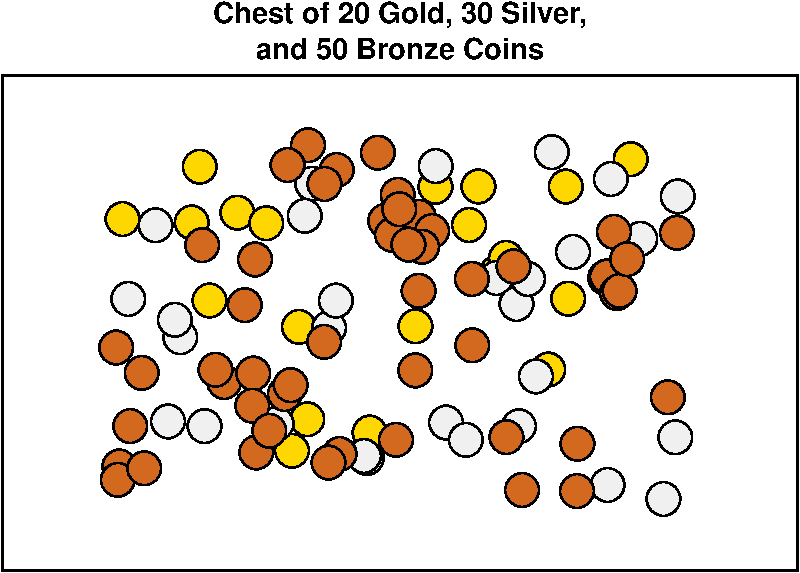
\includegraphics{YaRrr_files/figure-latex/unnamed-chunk-85-1.pdf}

Now, let's sample drawing coins from a treasure chest Let's say the
chest has 100 coins: 20 gold, 30 silver, and 50 bronze. Let's draw 10
random coins from this chest.

\begin{Shaded}
\begin{Highlighting}[]
\CommentTok{# Create chest with the 100 coins}

\NormalTok{chest <-}\StringTok{ }\KeywordTok{c}\NormalTok{(}\KeywordTok{rep}\NormalTok{(}\StringTok{"gold"}\NormalTok{, }\DecValTok{20}\NormalTok{),}
         \KeywordTok{rep}\NormalTok{(}\StringTok{"silver"}\NormalTok{, }\DecValTok{30}\NormalTok{),}
         \KeywordTok{rep}\NormalTok{(}\StringTok{"bronze"}\NormalTok{, }\DecValTok{50}\NormalTok{))}

\CommentTok{# Draw 10 coins from the chest}
\KeywordTok{sample}\NormalTok{(}\DataTypeTok{x =} \NormalTok{chest,}
       \DataTypeTok{size =} \DecValTok{10}\NormalTok{)}
\NormalTok{##  [1] "bronze" "silver" "bronze" "silver" "silver" "gold"   "gold"  }
\NormalTok{##  [8] "silver" "silver" "bronze"}
\end{Highlighting}
\end{Shaded}

The output of the \texttt{sample()} function above is a vector of 10
strings indicating the type of coin we drew on each sample. And like any
random sampling function, this code will likely give you different
results every time you run it! See how long it takes you to get 10 gold
coins\ldots{}

In the next section, we'll cover how to generate random data from
specified \emph{probability distributions}. What is a probability
distribution? Well, it's simply an equation -- also called a likelihood
function -- that indicates how likely certain numerical values are to be
drawn.

We can use probability distributions to represent different types of
data. For example, imagine you need to hire a new group of pirates for
your crew. You have the option of hiring people form one of two
different pirate training colleges that produce pirates of varying
quality. One college ``Pirate Training Unlimited'' might tend to pirates
that are generally ok - never great but never terrible. While another
college ``Unlimited Pirate Training'' might produce pirates with a wide
variety of quality, from very low to very high. In
Figure\textasciitilde{}\ref{fig:piratecollege} I plotted 5 example
pirates from each college, where each pirate is shown as a ball with a
number written on it. As you can see, pirates from PTU all tend to be
clustered between 40 and 60 (not terrible but not great), while pirates
from UPT are all over the map, from 0 to 100. We can use probability
distributions (in this case, the uniform distribution) to mathematically
define how likely any possible value is to be drawn at random from a
distribution. We could describe Pirate Training Unlimited with a uniform
distribution with a small range, and Unlimited Pirate Training with a
second uniform distribution with a wide range.

\begin{figure}[htbp]
\centering
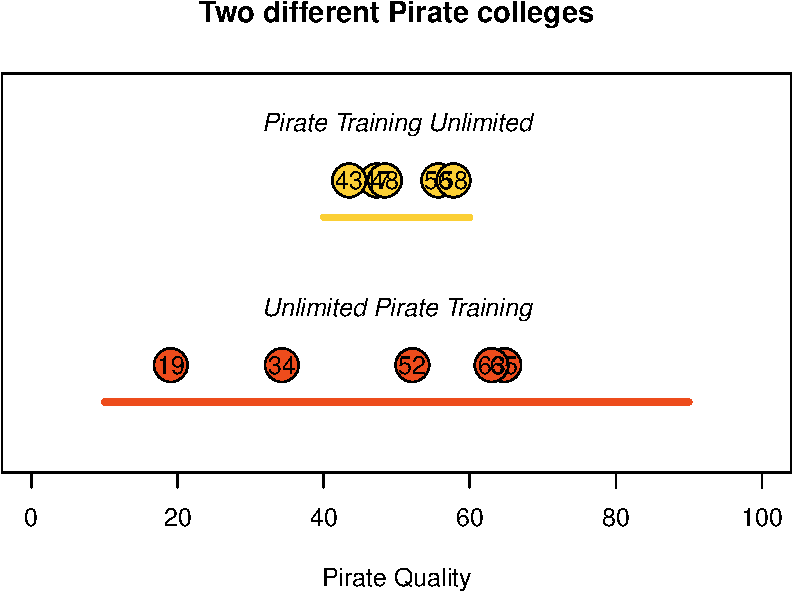
\includegraphics{YaRrr_files/figure-latex/piratecollege-1.pdf}
\caption{\label{fig:piratecollege}Sampling 5 potential pirates from two
different pirate colleges. Pirate Training Unlimited (PTU) consistently
produces average pirates (with scores between 40 and 60), while
Unlimited Pirate Training (UPT), produces a wide range of pirates from 0
to 100.}
\end{figure}

In the next two sections, I'll cover the two most common distributions:
The Normal and the Uniform. However, R contains many more distributions
than just these two. To see them all, look at the help menu for
Distributions:

\begin{Shaded}
\begin{Highlighting}[]
\CommentTok{# See all distributions included in Base R}
\NormalTok{?Distributions}
\end{Highlighting}
\end{Shaded}

\subsection{Normal (Gaussian)}\label{normal-gaussian}

\begin{figure}[htbp]
\centering
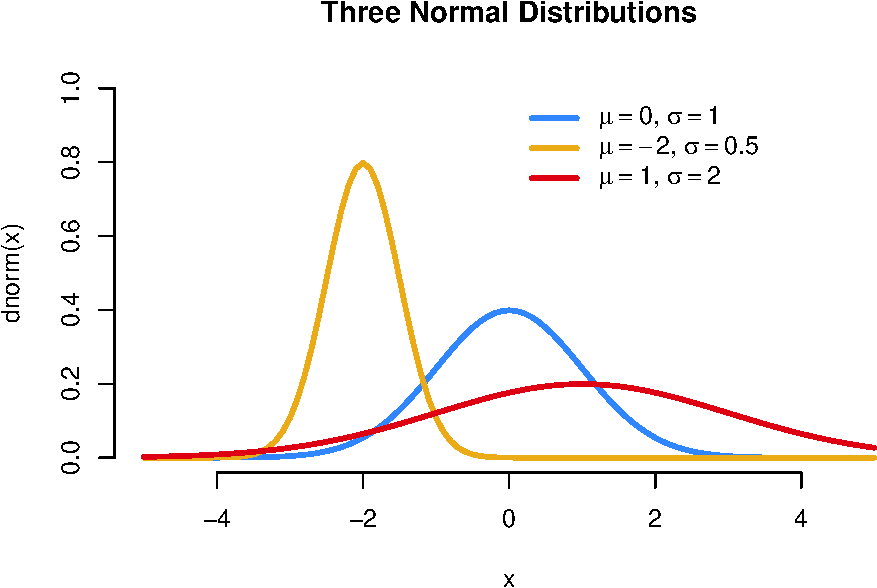
\includegraphics{YaRrr_files/figure-latex/normaldist-1.pdf}
\caption{\label{fig:normaldist}Three different normal distributions with
different means and standard deviations}
\end{figure}

\begin{longtable}[]{@{}ll@{}}
\toprule
Argument & Definition\tabularnewline
\midrule
\endhead
\texttt{n} & The number of observations to draw from the
distribution.\tabularnewline
\texttt{mean} & The mean of the distribution.\tabularnewline
\texttt{sd} & The standard deviation of the distribution.\tabularnewline
\bottomrule
\end{longtable}

The Normal (a.k.a ``Gaussian'') distribution is probably the most
important distribution in all of statistics. The Normal distribution is
bell-shaped, and has two parameters: a mean and a standard deviation. To
generate samples from a normal distribution in R, we use the function
\texttt{rnorm()}

\begin{Shaded}
\begin{Highlighting}[]
\CommentTok{# 5 samples from a Normal dist with mean = 0, sd = 1}
\KeywordTok{rnorm}\NormalTok{(}\DataTypeTok{n =} \DecValTok{5}\NormalTok{, }\DataTypeTok{mean =} \DecValTok{0}\NormalTok{, }\DataTypeTok{sd =} \DecValTok{1}\NormalTok{)}
\NormalTok{## [1]  0.54 -1.32 -0.16  0.16 -0.52}

\CommentTok{# 3 samples from a Normal dist with mean = -10, sd = 15}
\KeywordTok{rnorm}\NormalTok{(}\DataTypeTok{n =} \DecValTok{3}\NormalTok{, }\DataTypeTok{mean =} \NormalTok{-}\DecValTok{10}\NormalTok{, }\DataTypeTok{sd =} \DecValTok{15}\NormalTok{)}
\NormalTok{## [1] -42.0   5.2 -14.0}
\end{Highlighting}
\end{Shaded}

Again, because the sampling is done randomly, you'll get different
values each time you run \texttt{rnorm()}

\subsection{Uniform}\label{uniform}

\begin{figure}[htbp]
\centering
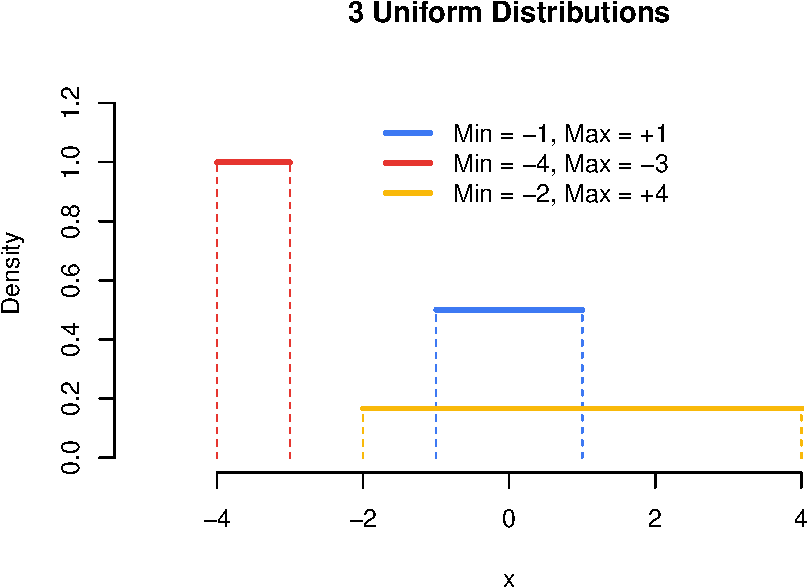
\includegraphics{YaRrr_files/figure-latex/uniformdist-1.pdf}
\caption{\label{fig:uniformdist}The Uniform distribution - known
colloquially as the Anthony Davis distribution.}
\end{figure}

Next, let's move on to the Uniform distribution. The Uniform
distribution gives equal probability to all values between its minimum
and maximum values. In other words, everything between its lower and
upper bounds are equally likely to occur. To generate samples from a
uniform distribution,use the function \texttt{runif()}, the function has
3 arguments:

\begin{longtable}[]{@{}ll@{}}
\toprule
\begin{minipage}[b]{0.14\columnwidth}\raggedright\strut
Argument\strut
\end{minipage} & \begin{minipage}[b]{0.61\columnwidth}\raggedright\strut
Definition\strut
\end{minipage}\tabularnewline
\midrule
\endhead
\begin{minipage}[t]{0.14\columnwidth}\raggedright\strut
\texttt{n}\strut
\end{minipage} & \begin{minipage}[t]{0.61\columnwidth}\raggedright\strut
The number of observations to draw from the distribution.\strut
\end{minipage}\tabularnewline
\begin{minipage}[t]{0.14\columnwidth}\raggedright\strut
\texttt{min}\strut
\end{minipage} & \begin{minipage}[t]{0.61\columnwidth}\raggedright\strut
The lower bound of the Uniform distribution from which samples are
drawn\strut
\end{minipage}\tabularnewline
\begin{minipage}[t]{0.14\columnwidth}\raggedright\strut
\texttt{max}\strut
\end{minipage} & \begin{minipage}[t]{0.61\columnwidth}\raggedright\strut
The upper bound of the Uniform distribution from which samples are
drawn\strut
\end{minipage}\tabularnewline
\bottomrule
\end{longtable}

Here are some samples from two different Uniform distributions:

\begin{Shaded}
\begin{Highlighting}[]
\CommentTok{# 5 samples from Uniform dist with bounds at 0 and 1}
\KeywordTok{runif}\NormalTok{(}\DataTypeTok{n =} \DecValTok{5}\NormalTok{, }\DataTypeTok{min =} \DecValTok{0}\NormalTok{, }\DataTypeTok{max =} \DecValTok{1}\NormalTok{)}
\NormalTok{## [1] 0.44 0.22 0.37 0.88 0.69}

\CommentTok{# 10 samples from Uniform dist with bounds at -100 and +100}
\KeywordTok{runif}\NormalTok{(}\DataTypeTok{n =} \DecValTok{10}\NormalTok{, }\DataTypeTok{min =} \NormalTok{-}\DecValTok{100}\NormalTok{, }\DataTypeTok{max =} \DecValTok{100}\NormalTok{)}
\NormalTok{##  [1]  63.7  43.9  62.5 -64.2 -99.0  12.2  20.8  62.5   5.6  11.1}
\end{Highlighting}
\end{Shaded}

\subsection{Notes on random samples}\label{notes-on-random-samples}

\subsubsection{Random samples will always
change}\label{random-samples-will-always-change}

Every time you draw a sample from a probability distribution, you'll
(likely) get a different result. For example, see what happens when I
run the following two commands (you'll learn the \texttt{rnorm()}
function on the next page\ldots{})

\begin{Shaded}
\begin{Highlighting}[]
\CommentTok{# Draw a sample of size 5 from a normal distribution with mean 100 and sd 10}
\KeywordTok{rnorm}\NormalTok{(}\DataTypeTok{n =} \DecValTok{5}\NormalTok{, }\DataTypeTok{mean =} \DecValTok{100}\NormalTok{, }\DataTypeTok{sd =} \DecValTok{10}\NormalTok{)}
\NormalTok{## [1] 113  90  98 109 113}

\CommentTok{# Do it again!}
\KeywordTok{rnorm}\NormalTok{(}\DataTypeTok{n =} \DecValTok{5}\NormalTok{, }\DataTypeTok{mean =} \DecValTok{100}\NormalTok{, }\DataTypeTok{sd =} \DecValTok{10}\NormalTok{)}
\NormalTok{## [1] 101  86  90 106  98}
\end{Highlighting}
\end{Shaded}

As you can see, the exact same code produced different results -- and
that's exactly what we want! Each time you run \texttt{rnorm()}, or
another distribution function, you'll get a new random sample.

\subsubsection{\texorpdfstring{Use \texttt{set.seed()} to control random
samples}{Use set.seed() to control random samples}}\label{use-set.seed-to-control-random-samples}

There will be cases where you will want to exert some control over the
random samples that R produces from sampling functions. For example, you
may want to create a reproducible example of some code that anyone else
can replicate exactly. To do this, use the \texttt{set.seed()} function.
Using \texttt{set.seed()} will force R to produce consistent random
samples at any time on any computer.

In the code below I'll set the sampling seed to 100 with
\texttt{set.seed(100)}. I'll then run \texttt{rnorm()} twice. The
results will always be consistent (because we fixed the sampling seed).

\begin{Shaded}
\begin{Highlighting}[]
\CommentTok{# Fix sampling seed to 100, so the next sampling functions}
\CommentTok{#   always produce the same values}
\KeywordTok{set.seed}\NormalTok{(}\DecValTok{100}\NormalTok{)}

\CommentTok{# The result will always be -0.5022, 0.1315, -0.0789}
\KeywordTok{rnorm}\NormalTok{(}\DecValTok{3}\NormalTok{, }\DataTypeTok{mean =} \DecValTok{0}\NormalTok{, }\DataTypeTok{sd =} \DecValTok{1}\NormalTok{)}
\NormalTok{## [1] -0.502  0.132 -0.079}

\CommentTok{# The result will always be 0.887, 0.117, 0.319}
\KeywordTok{rnorm}\NormalTok{(}\DecValTok{3}\NormalTok{, }\DataTypeTok{mean =} \DecValTok{0}\NormalTok{, }\DataTypeTok{sd =} \DecValTok{1}\NormalTok{)}
\NormalTok{## [1] 0.89 0.12 0.32}
\end{Highlighting}
\end{Shaded}

Try running the same code on your machine and you'll see the exact same
samples that I got above. Oh and the value of 100 I used above in
\texttt{set.seed(100)} is totally arbitrary -- you can set the seed to
any integer you want. I just happen to like how \texttt{set.seed(100)}
looks in my code.

\section{Test your R might!}\label{test-your-r-might-1}

\begin{enumerate}
\def\labelenumi{\arabic{enumi}.}
\item
  Create the vector {[}1, 2, 3, 4, 5, 6, 7, 8, 9, 10{]} in three ways:
  once using \texttt{c()}, once using \texttt{a:b}, and once using
  \texttt{seq()}.
\item
  Create the vector {[}2.1, 4.1, 6.1, 8.1{]} in two ways, once using
  \texttt{c()} and once using \texttt{seq()}
\item
  Create the vector {[}0, 5, 10, 15{]} in 3 ways: using \texttt{c()},
  \texttt{seq()} with a \texttt{by} argument, and \texttt{seq()} with a
  \texttt{length.out} argument.
\item
  Create the vector {[}101, 102, 103, 200, 205, 210, 1000, 1100, 1200{]}
  using a combination of the \texttt{c()} and \texttt{seq()} functions
\item
  A new batch of 100 pirates are boarding your ship and need new swords.
  You have 10 scimitars, 40 broadswords, and 50 cutlasses that you need
  to distribute evenly to the 100 pirates as they board. Create a vector
  of length 100 where there is 1 scimitar, 4 broadswords, and 5
  cutlasses in each group of 10. That is, in the first 10 elements there
  should be exactly 1 scimitar, 4 broadswords and 5 cutlasses. The next
  10 elements should also have the same number of each sword (and so
  on).
\item
  Create a vector that repeats the integers from 1 to 5, 10 times. That
  is {[}1, 2, 3, 4, 5, 1, 2, 3, 4, 5, \ldots{}{]}. The length of the
  vector should be 50!
\item
  Now, create the same vector as before, but this time repeat 1, 10
  times, then 2, 10 times, etc., That is {[}1, 1, 1, \ldots{}, 2, 2, 2,
  \ldots{}, \ldots{} 5, 5, 5{]}. The length of the vector should also be
  50
\item
  Create a vector containing 50 samples from a Normal distribution with
  a population mean of 20 and standard deviation of 2.
\item
  Create a vector containing 25 samples from a Uniform distribution with
  a lower bound of -100 and an upper bound of -50.
\end{enumerate}

\chapter{Vector functions}\label{vectorfunctions}

In this chapter, we'll cover the core functions for vector objects. The
code below uses the functions you'll learn to calculate summary
statistics from two exams.

\begin{figure}

{\centering 
\includegraphics[width=400px]{images/fuckexam} 

}

\end{figure}

\begin{Shaded}
\begin{Highlighting}[]
\CommentTok{# 10 students from two different classes took two exams.}
\CommentTok{#  Here are three vectors showing the data}
\NormalTok{midterm <-}\StringTok{ }\KeywordTok{c}\NormalTok{(}\DecValTok{62}\NormalTok{, }\DecValTok{68}\NormalTok{, }\DecValTok{75}\NormalTok{, }\DecValTok{79}\NormalTok{, }\DecValTok{55}\NormalTok{, }\DecValTok{62}\NormalTok{, }\DecValTok{89}\NormalTok{, }\DecValTok{76}\NormalTok{, }\DecValTok{45}\NormalTok{, }\DecValTok{67}\NormalTok{)}
\NormalTok{final <-}\StringTok{ }\KeywordTok{c}\NormalTok{(}\DecValTok{78}\NormalTok{, }\DecValTok{72}\NormalTok{, }\DecValTok{97}\NormalTok{, }\DecValTok{82}\NormalTok{, }\DecValTok{60}\NormalTok{, }\DecValTok{83}\NormalTok{, }\DecValTok{92}\NormalTok{, }\DecValTok{73}\NormalTok{, }\DecValTok{50}\NormalTok{, }\DecValTok{88}\NormalTok{)}

\CommentTok{# How many students are there?}
\KeywordTok{length}\NormalTok{(midterm)}
\NormalTok{## [1] 10}

\CommentTok{# Add 5 to each midterm score (extra credit!)}
\NormalTok{midterm <-}\StringTok{ }\NormalTok{midterm +}\StringTok{ }\DecValTok{5}
\NormalTok{midterm}
\NormalTok{##  [1] 67 73 80 84 60 67 94 81 50 72}

\CommentTok{# Difference between final and midterm scores}
\NormalTok{final -}\StringTok{ }\NormalTok{midterm}
\NormalTok{##  [1] 11 -1 17 -2  0 16 -2 -8  0 16}

\CommentTok{# Each student's average score}
\NormalTok{(midterm +}\StringTok{ }\NormalTok{final) /}\StringTok{ }\DecValTok{2}
\NormalTok{##  [1] 72 72 88 83 60 75 93 77 50 80}

\CommentTok{# Mean midterm grade}
\KeywordTok{mean}\NormalTok{(midterm)}
\NormalTok{## [1] 73}

\CommentTok{# Standard deviation of midterm grades}
\KeywordTok{sd}\NormalTok{(midterm)}
\NormalTok{## [1] 13}

\CommentTok{# Highest final grade}
\KeywordTok{max}\NormalTok{(final)}
\NormalTok{## [1] 97}

\CommentTok{# z-scores}
\NormalTok{midterm.z <-}\StringTok{ }\NormalTok{(midterm -}\StringTok{ }\KeywordTok{mean}\NormalTok{(midterm)) /}\StringTok{ }\KeywordTok{sd}\NormalTok{(midterm)}
\NormalTok{final.z <-}\StringTok{ }\NormalTok{(final -}\StringTok{ }\KeywordTok{mean}\NormalTok{(final)) /}\StringTok{ }\KeywordTok{sd}\NormalTok{(final)}
\end{Highlighting}
\end{Shaded}

\section{Arithmetic operations on
vectors}\label{arithmetic-operations-on-vectors}

So far, you know how to do basic arithmetic operations like +
(addition), - (subtraction), and * (multiplication) on scalars.
Thankfully, R makes it just as easy to do arithmetic operations on
numeric vectors:

\begin{Shaded}
\begin{Highlighting}[]
\NormalTok{a <-}\StringTok{ }\KeywordTok{c}\NormalTok{(}\DecValTok{1}\NormalTok{, }\DecValTok{2}\NormalTok{, }\DecValTok{3}\NormalTok{, }\DecValTok{4}\NormalTok{, }\DecValTok{5}\NormalTok{)}
\NormalTok{b <-}\StringTok{ }\KeywordTok{c}\NormalTok{(}\DecValTok{10}\NormalTok{, }\DecValTok{20}\NormalTok{, }\DecValTok{30}\NormalTok{, }\DecValTok{40}\NormalTok{, }\DecValTok{50}\NormalTok{)}

\NormalTok{a +}\StringTok{ }\DecValTok{100}
\NormalTok{## [1] 101 102 103 104 105}
\NormalTok{a +}\StringTok{ }\NormalTok{b}
\NormalTok{## [1] 11 22 33 44 55}
\NormalTok{(a +}\StringTok{ }\NormalTok{b) /}\StringTok{ }\DecValTok{10}
\NormalTok{## [1] 1.1 2.2 3.3 4.4 5.5}
\end{Highlighting}
\end{Shaded}

If you do an operation on a vector with a scalar, R will apply the
scalar to each element in the vector. For example, if you have a vector
and want to add 10 to each element in the vector, just add the vector
and scalar objects. Let's create a vector with the integers from 1 to
10, and add then add 100 to each element:

\begin{Shaded}
\begin{Highlighting}[]
\CommentTok{# Take the integers from 1 to 10, then add 100 to each}
\DecValTok{1}\NormalTok{:}\DecValTok{10} \NormalTok{+}\StringTok{ }\DecValTok{100}
\NormalTok{##  [1] 101 102 103 104 105 106 107 108 109 110}
\end{Highlighting}
\end{Shaded}

As you can see, the result is {[}1 + 100, 2 + 100, \ldots{} 10 + 100{]}.
Of course, we could have made this vector with the \texttt{a:b} function
like this: \texttt{101:110}, but you get the idea.

Of course, this doesn't only work with addition\ldots{}oh no. Let's try
division, multiplication, and exponents. Let's create a vector
\texttt{a} with the integers from 1 to 10 and then change it up:

\begin{Shaded}
\begin{Highlighting}[]
\NormalTok{a <-}\StringTok{ }\DecValTok{1}\NormalTok{:}\DecValTok{10}
\NormalTok{a /}\StringTok{ }\DecValTok{100}
\NormalTok{##  [1] 0.01 0.02 0.03 0.04 0.05 0.06 0.07 0.08 0.09 0.10}
\NormalTok{a ^}\StringTok{ }\DecValTok{2}
\NormalTok{##  [1]   1   4   9  16  25  36  49  64  81 100}
\end{Highlighting}
\end{Shaded}

Again, if you perform an algebraic operation on a vector with a scalar,
R will just apply the operation to every element in the vector.

\subsection{Basic math with multiple
vectors}\label{basic-math-with-multiple-vectors}

What if you want to do some operation on two vectors of the same length?
Easy. Just apply the operation to both vectors. R will then combine them
element--by--element. For example, if you add the vector {[}1, 2, 3, 4,
5{]} to the vector {[}5, 4, 3, 2, 1{]}, the resulting vector will have
the values {[}1 + 5, 2 + 4, 3 + 3, 4 + 2, 5 + 1{]} = {[}6, 6, 6, 6,
6{]}:

\begin{Shaded}
\begin{Highlighting}[]
\KeywordTok{c}\NormalTok{(}\DecValTok{1}\NormalTok{, }\DecValTok{2}\NormalTok{, }\DecValTok{3}\NormalTok{, }\DecValTok{4}\NormalTok{, }\DecValTok{5}\NormalTok{) +}\StringTok{ }\KeywordTok{c}\NormalTok{(}\DecValTok{5}\NormalTok{, }\DecValTok{4}\NormalTok{, }\DecValTok{3}\NormalTok{, }\DecValTok{2}\NormalTok{, }\DecValTok{1}\NormalTok{)}
\NormalTok{## [1] 6 6 6 6 6}
\end{Highlighting}
\end{Shaded}

Let's create two vectors a and b where each vector contains the integers
from 1 to 5. We'll then create two new vectors \texttt{ab.sum}, the sum
of the two vectors and \texttt{ab.diff}, the difference of the two
vectors, and \texttt{ab.prod}, the product of the two vectors:

\begin{Shaded}
\begin{Highlighting}[]
\NormalTok{a <-}\StringTok{ }\DecValTok{1}\NormalTok{:}\DecValTok{5}
\NormalTok{b <-}\StringTok{ }\DecValTok{1}\NormalTok{:}\DecValTok{5}

\NormalTok{ab.sum <-}\StringTok{ }\NormalTok{a +}\StringTok{ }\NormalTok{b}
\NormalTok{ab.diff <-}\StringTok{ }\NormalTok{a -}\StringTok{ }\NormalTok{b}
\NormalTok{ab.prod <-}\StringTok{ }\NormalTok{a *}\StringTok{ }\NormalTok{b}

\NormalTok{ab.sum}
\NormalTok{## [1]  2  4  6  8 10}
\NormalTok{ab.diff}
\NormalTok{## [1] 0 0 0 0 0}
\NormalTok{ab.prod}
\NormalTok{## [1]  1  4  9 16 25}
\end{Highlighting}
\end{Shaded}

\subsection{Ex: Pirate Bake Sale}\label{ex-pirate-bake-sale}

\begin{figure}

{\centering 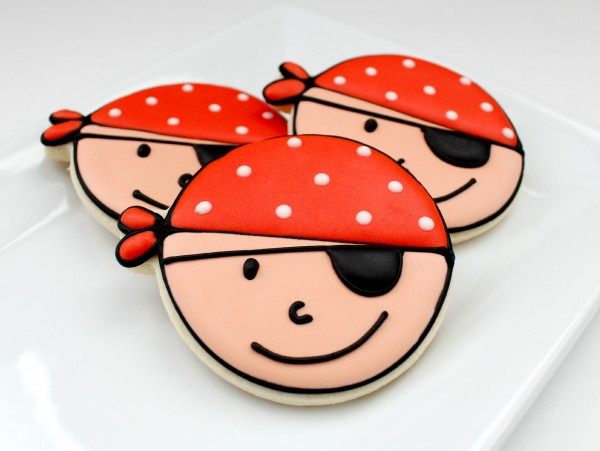
\includegraphics[width=400px]{images/piratecookies} 

}

\end{figure}

Let's say you had a bake sale on your ship where 5 pirates sold both
pies and cookies. You could record the total number of pies and cookies
sold in two vectors:

\begin{Shaded}
\begin{Highlighting}[]
\NormalTok{pies <-}\StringTok{ }\KeywordTok{c}\NormalTok{(}\DecValTok{3}\NormalTok{, }\DecValTok{6}\NormalTok{, }\DecValTok{2}\NormalTok{, }\DecValTok{10}\NormalTok{, }\DecValTok{4}\NormalTok{)}
\NormalTok{cookies <-}\StringTok{ }\KeywordTok{c}\NormalTok{(}\DecValTok{70}\NormalTok{, }\DecValTok{40}\NormalTok{, }\DecValTok{40}\NormalTok{, }\DecValTok{200}\NormalTok{, }\DecValTok{60}\NormalTok{)}
\end{Highlighting}
\end{Shaded}

Now, let's say you want to know how many total items each pirate sold.
You can do this by just adding the two vectors:

\begin{Shaded}
\begin{Highlighting}[]
\NormalTok{total.sold <-}\StringTok{ }\NormalTok{pies +}\StringTok{ }\NormalTok{cookies}
\NormalTok{total.sold}
\NormalTok{## [1]  73  46  42 210  64}
\end{Highlighting}
\end{Shaded}

Crazy.

\section{Summary statistics}\label{summary-statistics}

Ok, now that we can create vectors, let's learn the basic descriptive
statistics functions. We'll start with functions that apply to
continuous data. Continuous data is data that, generally speaking, can
take on an infinite number of values. Height and weight are good
examples of continuous data. Table
\ref{tab:continuousvectorfunctiontable} contains common functions for
continuous, numeric vectors. Each of them takes a numeric vector as an
argument, and returns either a scalar (or in the case of
\texttt{summary()}, a \texttt{table}) as a result.

\begin{longtable}[]{@{}lll@{}}
\caption{\label{tab:continuousvectorfunctiontable} Summary statistic
functions for continuous data.}\tabularnewline
\toprule
\begin{minipage}[b]{0.27\columnwidth}\raggedright\strut
Function\strut
\end{minipage} & \begin{minipage}[b]{0.30\columnwidth}\raggedright\strut
Example\strut
\end{minipage} & \begin{minipage}[b]{0.32\columnwidth}\raggedright\strut
Result\strut
\end{minipage}\tabularnewline
\midrule
\endfirsthead
\toprule
\begin{minipage}[b]{0.27\columnwidth}\raggedright\strut
Function\strut
\end{minipage} & \begin{minipage}[b]{0.30\columnwidth}\raggedright\strut
Example\strut
\end{minipage} & \begin{minipage}[b]{0.32\columnwidth}\raggedright\strut
Result\strut
\end{minipage}\tabularnewline
\midrule
\endhead
\begin{minipage}[t]{0.27\columnwidth}\raggedright\strut
\texttt{sum(x),\ product(x)}\strut
\end{minipage} & \begin{minipage}[t]{0.30\columnwidth}\raggedright\strut
\texttt{sum(1:10)}\strut
\end{minipage} & \begin{minipage}[t]{0.32\columnwidth}\raggedright\strut
55\strut
\end{minipage}\tabularnewline
\begin{minipage}[t]{0.27\columnwidth}\raggedright\strut
\texttt{min(x),\ max(x)}\strut
\end{minipage} & \begin{minipage}[t]{0.30\columnwidth}\raggedright\strut
\texttt{min(1:10)}\strut
\end{minipage} & \begin{minipage}[t]{0.32\columnwidth}\raggedright\strut
1\strut
\end{minipage}\tabularnewline
\begin{minipage}[t]{0.27\columnwidth}\raggedright\strut
\texttt{mean(x),\ median(x)}\strut
\end{minipage} & \begin{minipage}[t]{0.30\columnwidth}\raggedright\strut
\texttt{mean(1:10)}\strut
\end{minipage} & \begin{minipage}[t]{0.32\columnwidth}\raggedright\strut
5.5\strut
\end{minipage}\tabularnewline
\begin{minipage}[t]{0.27\columnwidth}\raggedright\strut
\texttt{sd(x),\ var(x),\ range(x)}\strut
\end{minipage} & \begin{minipage}[t]{0.30\columnwidth}\raggedright\strut
\texttt{sd(1:10)}\strut
\end{minipage} & \begin{minipage}[t]{0.32\columnwidth}\raggedright\strut
3.03\strut
\end{minipage}\tabularnewline
\begin{minipage}[t]{0.27\columnwidth}\raggedright\strut
\texttt{quantile(x,\ probs)}\strut
\end{minipage} & \begin{minipage}[t]{0.30\columnwidth}\raggedright\strut
\texttt{quantile(1:10,\ probs\ =\ .2)}\strut
\end{minipage} & \begin{minipage}[t]{0.32\columnwidth}\raggedright\strut
2.8\strut
\end{minipage}\tabularnewline
\begin{minipage}[t]{0.27\columnwidth}\raggedright\strut
\texttt{summary(x)}\strut
\end{minipage} & \begin{minipage}[t]{0.30\columnwidth}\raggedright\strut
\texttt{summary(1:10)}\strut
\end{minipage} & \begin{minipage}[t]{0.32\columnwidth}\raggedright\strut
\texttt{Min\ =\ 1.00.\ 1st\ Qu.\ =\ 3.25,\ Median\ =\ 5.50,\ Mean\ =\ 5.50,\ 3rd\ Qu.\ =\ 7.75,\ Max\ =\ 10.0}\strut
\end{minipage}\tabularnewline
\bottomrule
\end{longtable}

Let's calculate some descriptive statistics from some pirate related
data. I'll create a vector called \texttt{x} that contains the number of
tattoos from 10 random pirates.

\begin{Shaded}
\begin{Highlighting}[]
\NormalTok{tattoos <-}\StringTok{ }\KeywordTok{c}\NormalTok{(}\DecValTok{4}\NormalTok{, }\DecValTok{50}\NormalTok{, }\DecValTok{2}\NormalTok{, }\DecValTok{39}\NormalTok{, }\DecValTok{4}\NormalTok{, }\DecValTok{20}\NormalTok{, }\DecValTok{4}\NormalTok{, }\DecValTok{8}\NormalTok{, }\DecValTok{10}\NormalTok{, }\DecValTok{100}\NormalTok{)}
\end{Highlighting}
\end{Shaded}

Now, we can calculate several descriptive statistics on this vector by
using the summary statistics functions:

\begin{Shaded}
\begin{Highlighting}[]
\KeywordTok{min}\NormalTok{(tattoos)}
\NormalTok{## [1] 2}
\KeywordTok{mean}\NormalTok{(tattoos)}
\NormalTok{## [1] 24}
\KeywordTok{sd}\NormalTok{(tattoos)}
\NormalTok{## [1] 31}
\end{Highlighting}
\end{Shaded}

\subsection{length()}\label{length}

\begin{figure}

{\centering 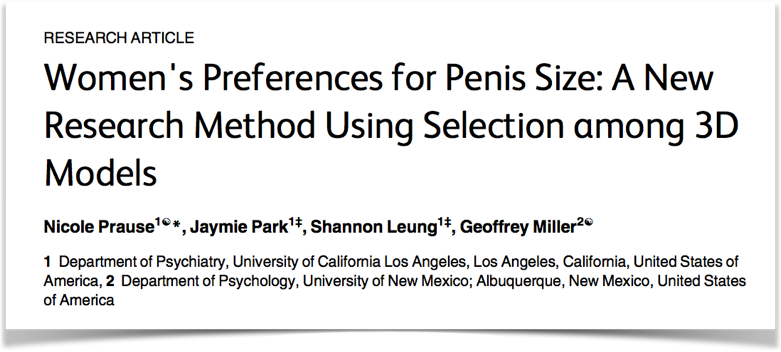
\includegraphics[width=400px]{images/penissize} 

}

\caption{According to this article published in 2015 in Plos One, when it comes to people, length may matter for some. But trust me, for vectors it always does.}\label{fig:unnamed-chunk-105}
\end{figure}

Vectors have one dimension: their length. Later on, when you combine
vectors into more higher dimensional objects, like matrices and
dataframes, you will need to make sure that all the vectors you combine
have the same length. But, when you want to know the length of a vector,
don't stare at your computer screen and count the elements one by one!
(That said, I must admit that I still do this sometimes\ldots{}).
Instead, use \texttt{length()} function. The \texttt{length()} function
takes a vector as an argument, and returns a scalar representing the
number of elements in the vector:

\begin{Shaded}
\begin{Highlighting}[]
\NormalTok{a <-}\StringTok{ }\DecValTok{1}\NormalTok{:}\DecValTok{10}
\KeywordTok{length}\NormalTok{(a)  }\CommentTok{# How many elements are in a?}
\NormalTok{## [1] 10}

\NormalTok{b <-}\StringTok{ }\KeywordTok{seq}\NormalTok{(}\DataTypeTok{from =} \DecValTok{1}\NormalTok{, }\DataTypeTok{to =} \DecValTok{100}\NormalTok{, }\DataTypeTok{length.out =} \DecValTok{20}\NormalTok{)}
\KeywordTok{length}\NormalTok{(b)  }\CommentTok{# How many elements are in b?}
\NormalTok{## [1] 20}

\KeywordTok{length}\NormalTok{(}\KeywordTok{c}\NormalTok{(}\StringTok{"This"}\NormalTok{, }\StringTok{"character"}\NormalTok{, }\StringTok{"vector"}\NormalTok{, }\StringTok{"has"}\NormalTok{, }\StringTok{"six"}\NormalTok{, }\StringTok{"elements."}\NormalTok{))}
\NormalTok{## [1] 6}
\KeywordTok{length}\NormalTok{(}\StringTok{"This character scalar has just one element."}\NormalTok{)}
\NormalTok{## [1] 1}
\end{Highlighting}
\end{Shaded}

Get used to the \texttt{length()} function people, you'll be using it a
lot!

\subsection{Additional numeric vector
functions}\label{additional-numeric-vector-functions}

Table \ref{tab:morenumericfunctions} contains additional functions that
you will find useful when managing numeric vectors:

\begin{longtable}[]{@{}llll@{}}
\caption{\label{tab:morenumericfunctions} Vector summary functions for
continuous data.}\tabularnewline
\toprule
\begin{minipage}[b]{0.17\columnwidth}\raggedright\strut
Function\strut
\end{minipage} & \begin{minipage}[b]{0.24\columnwidth}\raggedright\strut
Description\strut
\end{minipage} & \begin{minipage}[b]{0.33\columnwidth}\raggedright\strut
Example\strut
\end{minipage} & \begin{minipage}[b]{0.15\columnwidth}\raggedright\strut
Result\strut
\end{minipage}\tabularnewline
\midrule
\endfirsthead
\toprule
\begin{minipage}[b]{0.17\columnwidth}\raggedright\strut
Function\strut
\end{minipage} & \begin{minipage}[b]{0.24\columnwidth}\raggedright\strut
Description\strut
\end{minipage} & \begin{minipage}[b]{0.33\columnwidth}\raggedright\strut
Example\strut
\end{minipage} & \begin{minipage}[b]{0.15\columnwidth}\raggedright\strut
Result\strut
\end{minipage}\tabularnewline
\midrule
\endhead
\begin{minipage}[t]{0.17\columnwidth}\raggedright\strut
\texttt{round(x,\ digits)}\strut
\end{minipage} & \begin{minipage}[t]{0.24\columnwidth}\raggedright\strut
Round elements in x to \texttt{digits} digits\strut
\end{minipage} & \begin{minipage}[t]{0.33\columnwidth}\raggedright\strut
\texttt{round(c(2.231,\ 3.1415),\ digits\ =\ 1)}\strut
\end{minipage} & \begin{minipage}[t]{0.15\columnwidth}\raggedright\strut
2.2, 3.1\strut
\end{minipage}\tabularnewline
\begin{minipage}[t]{0.17\columnwidth}\raggedright\strut
\texttt{ceiling(x),\ floor(x)}\strut
\end{minipage} & \begin{minipage}[t]{0.24\columnwidth}\raggedright\strut
Round elements x to the next highest (or lowest) integer\strut
\end{minipage} & \begin{minipage}[t]{0.33\columnwidth}\raggedright\strut
\texttt{ceiling(c(5.1,\ 7.9))}\strut
\end{minipage} & \begin{minipage}[t]{0.15\columnwidth}\raggedright\strut
6, 8\strut
\end{minipage}\tabularnewline
\begin{minipage}[t]{0.17\columnwidth}\raggedright\strut
\texttt{x\ \%\%\ y}\strut
\end{minipage} & \begin{minipage}[t]{0.24\columnwidth}\raggedright\strut
Modular arithmetic (ie. x mod y)\strut
\end{minipage} & \begin{minipage}[t]{0.33\columnwidth}\raggedright\strut
\texttt{7\ \%\%\ 3}\strut
\end{minipage} & \begin{minipage}[t]{0.15\columnwidth}\raggedright\strut
1\strut
\end{minipage}\tabularnewline
\bottomrule
\end{longtable}

\subsection{Sample statistics from random
samples}\label{sample-statistics-from-random-samples}

Now that you know how to calculate summary statistics, let's take a
closer look at how R draws random samples using the \texttt{rnorm()} and
\texttt{runif()} functions. In the next code chunk, I'll calculate some
summary statistics from a vector of 5 values from a Normal distribution
with a mean of 10 and a standard deviation of 5. I'll then calculate
summary statistics from this sample using \texttt{mean()} and
\texttt{sd()}:

\begin{Shaded}
\begin{Highlighting}[]
\CommentTok{# 5 samples from a Normal dist with mean = 10 and sd = 5}
\NormalTok{x <-}\StringTok{ }\KeywordTok{rnorm}\NormalTok{(}\DataTypeTok{n =} \DecValTok{5}\NormalTok{, }\DataTypeTok{mean =} \DecValTok{10}\NormalTok{, }\DataTypeTok{sd =} \DecValTok{5}\NormalTok{)}

\CommentTok{# What are the mean and standard deviation of the sample?}
\KeywordTok{mean}\NormalTok{(x)}
\NormalTok{## [1] 11}
\KeywordTok{sd}\NormalTok{(x)}
\NormalTok{## [1] 2.5}
\end{Highlighting}
\end{Shaded}

As you can see, the mean and standard deviation of our sample vector are
close to the population values of 10 and 5 -- but they aren't exactly
the same because these are sample data. If we take a much larger sample
(say, 100,000), the sample statistics should get much closer to the
population values:

\begin{Shaded}
\begin{Highlighting}[]
\CommentTok{# 100,000 samples from a Normal dist with mean = 10, sd = 5}
\NormalTok{y <-}\StringTok{ }\KeywordTok{rnorm}\NormalTok{(}\DataTypeTok{n =} \DecValTok{100000}\NormalTok{, }\DataTypeTok{mean =} \DecValTok{10}\NormalTok{, }\DataTypeTok{sd =} \DecValTok{5}\NormalTok{)}

\KeywordTok{mean}\NormalTok{(y)}
\NormalTok{## [1] 10}
\KeywordTok{sd}\NormalTok{(y)}
\NormalTok{## [1] 5}
\end{Highlighting}
\end{Shaded}

Yep, sure enough our new sample y (containing 100,000 values) has a
sample mean and standard deviation much closer (almost identical) to the
population values than our sample x (containing only 5 values). This is
an example of what is called the law of large numbers. Google it.

\section{Counting statistics}\label{counting-statistics}

Next, we'll move on to common counting functions for vectors with
discrete or non-numeric data. Discrete data are those like gender,
occupation, and monkey farts, that only allow for a finite (or at least,
plausibly finite) set of responses. Common functions for discrete
vectors are in Table \ref{tab:discretevectorfunctiontable}. Each of
these vectors takes a vector as an argument -- however, unlike the
previous functions we looked at, the used as arguments to these
functions can be either numeric or character.

\begin{longtable}[]{@{}llll@{}}
\caption{\label{tab:discretevectorfunctiontable} Counting functions for
discrete data.}\tabularnewline
\toprule
\begin{minipage}[b]{0.13\columnwidth}\raggedright\strut
Function\strut
\end{minipage} & \begin{minipage}[b]{0.23\columnwidth}\raggedright\strut
Description\strut
\end{minipage} & \begin{minipage}[b]{0.29\columnwidth}\raggedright\strut
Example\strut
\end{minipage} & \begin{minipage}[b]{0.23\columnwidth}\raggedright\strut
Result\strut
\end{minipage}\tabularnewline
\midrule
\endfirsthead
\toprule
\begin{minipage}[b]{0.13\columnwidth}\raggedright\strut
Function\strut
\end{minipage} & \begin{minipage}[b]{0.23\columnwidth}\raggedright\strut
Description\strut
\end{minipage} & \begin{minipage}[b]{0.29\columnwidth}\raggedright\strut
Example\strut
\end{minipage} & \begin{minipage}[b]{0.23\columnwidth}\raggedright\strut
Result\strut
\end{minipage}\tabularnewline
\midrule
\endhead
\begin{minipage}[t]{0.13\columnwidth}\raggedright\strut
\texttt{unique(x)}\strut
\end{minipage} & \begin{minipage}[t]{0.23\columnwidth}\raggedright\strut
Returns a vector of all unique values.\strut
\end{minipage} & \begin{minipage}[t]{0.29\columnwidth}\raggedright\strut
\texttt{unique(c(1,\ 1,\ 2,\ 10))}\strut
\end{minipage} & \begin{minipage}[t]{0.23\columnwidth}\raggedright\strut
1, 2, 10\strut
\end{minipage}\tabularnewline
\begin{minipage}[t]{0.13\columnwidth}\raggedright\strut
\texttt{table(x,\ exclude)}\strut
\end{minipage} & \begin{minipage}[t]{0.23\columnwidth}\raggedright\strut
Returns a table showing all the unique values as well as a count of each
occurrence. To include a count of NA values, include the argument
\texttt{exclude\ =\ NULL}\strut
\end{minipage} & \begin{minipage}[t]{0.29\columnwidth}\raggedright\strut
\texttt{table(c("a",\ "a",\ "b",\ "c"))}\strut
\end{minipage} & \begin{minipage}[t]{0.23\columnwidth}\raggedright\strut
\texttt{2-"a",\ 1-"b",\ 1-"c"}\strut
\end{minipage}\tabularnewline
\bottomrule
\end{longtable}

Let's test these functions by starting with two vectors of discrete
data:

\begin{Shaded}
\begin{Highlighting}[]
\NormalTok{vec <-}\StringTok{ }\KeywordTok{c}\NormalTok{(}\DecValTok{1}\NormalTok{, }\DecValTok{1}\NormalTok{, }\DecValTok{1}\NormalTok{, }\DecValTok{5}\NormalTok{, }\DecValTok{1}\NormalTok{, }\DecValTok{1}\NormalTok{, }\DecValTok{10}\NormalTok{, }\DecValTok{10}\NormalTok{, }\DecValTok{10}\NormalTok{)}
\NormalTok{gender <-}\StringTok{ }\KeywordTok{c}\NormalTok{(}\StringTok{"M"}\NormalTok{, }\StringTok{"M"}\NormalTok{, }\StringTok{"F"}\NormalTok{, }\StringTok{"F"}\NormalTok{, }\StringTok{"F"}\NormalTok{, }\StringTok{"M"}\NormalTok{, }\StringTok{"F"}\NormalTok{, }\StringTok{"M"}\NormalTok{, }\StringTok{"F"}\NormalTok{)}
\end{Highlighting}
\end{Shaded}

The function \texttt{unique(x)} will tell you all the unique values in
the vector, but won't tell you anything about how often each value
occurs.

\begin{Shaded}
\begin{Highlighting}[]
\KeywordTok{unique}\NormalTok{(vec)}
\NormalTok{## [1]  1  5 10}
\KeywordTok{unique}\NormalTok{(gender)}
\NormalTok{## [1] "M" "F"}
\end{Highlighting}
\end{Shaded}

The function \texttt{table()} does the same thing as \texttt{unique()},
but goes a step further in telling you how often each of the unique
values occurs:

\begin{Shaded}
\begin{Highlighting}[]
\KeywordTok{table}\NormalTok{(vec)}
\NormalTok{## vec}
\NormalTok{##  1  5 10 }
\NormalTok{##  5  1  3}
\KeywordTok{table}\NormalTok{(gender)}
\NormalTok{## gender}
\NormalTok{## F M }
\NormalTok{## 5 4}
\end{Highlighting}
\end{Shaded}

If you want to get a table of percentages instead of counts, you can
just divide the result of the \texttt{table()} function by the sum of
the result:

\begin{Shaded}
\begin{Highlighting}[]
\KeywordTok{table}\NormalTok{(vec) /}\StringTok{ }\KeywordTok{sum}\NormalTok{(}\KeywordTok{table}\NormalTok{(vec))}
\NormalTok{## vec}
\NormalTok{##    1    5   10 }
\NormalTok{## 0.56 0.11 0.33}
\KeywordTok{table}\NormalTok{(gender) /}\StringTok{ }\KeywordTok{sum}\NormalTok{(}\KeywordTok{table}\NormalTok{(gender))}
\NormalTok{## gender}
\NormalTok{##    F    M }
\NormalTok{## 0.56 0.44}
\end{Highlighting}
\end{Shaded}

\section{Missing (NA) values}\label{missing-na-values}

In R, missing data are coded as NA. In real datasets, NA values turn up
all the time. Unfortunately, most descriptive statistics functions will
freak out if there is a missing (NA) value in the data. For example, the
following code will return NA as a result because there is an NA value
in the data vector:

\begin{Shaded}
\begin{Highlighting}[]
\NormalTok{a <-}\StringTok{ }\KeywordTok{c}\NormalTok{(}\DecValTok{1}\NormalTok{, }\DecValTok{5}\NormalTok{, }\OtherTok{NA}\NormalTok{, }\DecValTok{2}\NormalTok{, }\DecValTok{10}\NormalTok{)}
\KeywordTok{mean}\NormalTok{(a)}
\NormalTok{## [1] NA}
\end{Highlighting}
\end{Shaded}

Thankfully, there's a way we can work around this. To tell a descriptive
statistic function to ignore missing (NA) values, include the argument
\texttt{na.rm\ =\ TRUE} in the function. This argument explicitly tells
the function to ignore NA values. Let's try calculating the mean of the
vector \texttt{a} again, this time with the
additional\texttt{na.rm\ =\ TRUE} argument:

\begin{Shaded}
\begin{Highlighting}[]
\KeywordTok{mean}\NormalTok{(a, }\DataTypeTok{na.rm =} \OtherTok{TRUE}\NormalTok{)}
\NormalTok{## [1] 4.5}
\end{Highlighting}
\end{Shaded}

Now, the function ignored the NA value and returned the mean of the
remaining data. While this may seem trivial now (why did we include an
NA value in the vector if we wanted to ignore it?!), it will be become
very important when we apply the function to real data which, very
often, contains missing values.

\section{Standardization (z-score)}\label{standardization-z-score}

A common task in statistics is to standardize variables -- also known as
calculating z-scores. The purpose of standardizing a vector is to put it
on a common scale which allows you to compare it to other (standardized)
variables. To standardize a vector, you simply subtract the vector by
its mean, and then divide the result by the vector's standard deviation.

If the concept of z-scores is new to you -- don't worry. In the next
worked example, you'll see how it can help you compare two sets of data.
But for now, let's see how easy it is to standardize a vector using
basic arithmetic.

Let's say you have a vector a containing some data. We'll assign the
vector to a new object called \texttt{a} then calculate the mean and
standard deviation with the \texttt{mean()} and \texttt{sd()} functions:

\begin{Shaded}
\begin{Highlighting}[]
\NormalTok{a <-}\StringTok{ }\KeywordTok{c}\NormalTok{(}\DecValTok{5}\NormalTok{, }\DecValTok{3}\NormalTok{, }\DecValTok{7}\NormalTok{, }\DecValTok{5}\NormalTok{, }\DecValTok{5}\NormalTok{, }\DecValTok{3}\NormalTok{, }\DecValTok{4}\NormalTok{)}
\KeywordTok{mean}\NormalTok{(a)}
\NormalTok{## [1] 4.6}
\KeywordTok{sd}\NormalTok{(a)}
\NormalTok{## [1] 1.4}
\end{Highlighting}
\end{Shaded}

Ok. Now we'll create a new vector called \texttt{a.z} which is a
standardized version of a. To do this, we'll simply subtract the mean of
the vector, then divide by the standard deviation.

\begin{Shaded}
\begin{Highlighting}[]
\NormalTok{a.z <-}\StringTok{ }\NormalTok{(a -}\StringTok{ }\KeywordTok{mean}\NormalTok{(a)) /}\StringTok{ }\KeywordTok{sd}\NormalTok{(a)}
\end{Highlighting}
\end{Shaded}

Now let's look at the standardized values:

\begin{Shaded}
\begin{Highlighting}[]
\NormalTok{a.z}
\NormalTok{## [1]  0.31 -1.12  1.74  0.31  0.31 -1.12 -0.41}
\end{Highlighting}
\end{Shaded}

The mean of \texttt{a.z} should now be 0, and the standard deviation of
\texttt{a.z} should now be 1. Let's make sure:

\begin{Shaded}
\begin{Highlighting}[]
\KeywordTok{mean}\NormalTok{(a.z)}
\NormalTok{## [1] 2e-16}
\KeywordTok{sd}\NormalTok{(a.z)}
\NormalTok{## [1] 1}
\end{Highlighting}
\end{Shaded}

Sweet. Oh, don't worry that the mean of \texttt{a.z} doesn't look like
exactly zero. Using non-scientific notation, the result is
0.000000000000000198. For all intents and purposes, that's 0. The reason
the result is not exactly 0 is due to computer science theoretical
reasons that I cannot explain (because I don't understand them).

\subsection{Ex: Evaluating a
competition}\label{ex-evaluating-a-competition}

Your gluten-intolerant first mate just perished in a tragic soy sauce
incident and it's time to promote another member of your crew to the
newly vacated position. Of course, only two qualities really matter for
a pirate: rope-climbing, and grogg drinking. Therefore, to see which of
your crew deserves the promotion, you decide to hold a climbing and
drinking competition. In the climbing competition, you measure how many
feet of rope a pirate can climb in an hour. In the drinking competition,
you measure how many mugs of grogg they can drink in a minute. Five
pirates volunteer for the competition -- here are their results:

\begin{table}

\caption{\label{tab:unnamed-chunk-120}Scores from a pirate competition}
\centering
\begin{tabular}[t]{l|r|r}
\hline
pirate & grogg & climbing\\
\hline
Heidi & 12 & 100\\
\hline
Andrew & 8 & 520\\
\hline
Becki & 1 & 430\\
\hline
Madisen & 6 & 200\\
\hline
David & 2 & 700\\
\hline
\end{tabular}
\end{table}

We can represent the main results with two vectors \texttt{grogg} and
\texttt{climbing}:

\begin{Shaded}
\begin{Highlighting}[]
\NormalTok{grogg <-}\StringTok{ }\KeywordTok{c}\NormalTok{(}\DecValTok{12}\NormalTok{, }\DecValTok{8}\NormalTok{, }\DecValTok{1}\NormalTok{, }\DecValTok{6}\NormalTok{, }\DecValTok{2}\NormalTok{)}
\NormalTok{climbing <-}\StringTok{ }\KeywordTok{c}\NormalTok{(}\DecValTok{100}\NormalTok{, }\DecValTok{520}\NormalTok{, }\DecValTok{430}\NormalTok{, }\DecValTok{200}\NormalTok{, }\DecValTok{700}\NormalTok{)}
\end{Highlighting}
\end{Shaded}

Now you've got the data, but there's a problem: the scales of the
numbers are very different. While the grogg numbers range from 1 to 12,
the climbing numbers have a much larger range from 100 to 700. This
makes it difficult to compare the two sets of numbers directly.

To solve this problem, we'll use standardization. Let's create new
standardized vectors called \texttt{grogg.z} and \texttt{climbing.z}

\begin{Shaded}
\begin{Highlighting}[]
\NormalTok{grogg.z <-}\StringTok{ }\NormalTok{(grogg -}\StringTok{ }\KeywordTok{mean}\NormalTok{(grogg)) /}\StringTok{ }\KeywordTok{sd}\NormalTok{(grogg)}
\NormalTok{climbing.z <-}\StringTok{ }\NormalTok{(climbing -}\StringTok{ }\KeywordTok{mean}\NormalTok{(climbing)) /}\StringTok{ }\KeywordTok{sd}\NormalTok{(climbing)}
\end{Highlighting}
\end{Shaded}

Now let's look at the final results

\begin{Shaded}
\begin{Highlighting}[]
\NormalTok{grogg.z}
\NormalTok{## [1]  1.379  0.489 -1.068  0.044 -0.845}
\NormalTok{climbing.z}
\NormalTok{## [1] -1.20  0.54  0.17 -0.78  1.28}
\end{Highlighting}
\end{Shaded}

It looks like there were two outstanding performances in particular. In
the grogg drinking competition, the first pirate (Heidi) had a z-score
of 1.4. We can interpret this by saying that Heidi drank 1.4 more
standard deviations of mugs of grogg than the average pirate. In the
climbing competition, the fifth pirate (David) had a z-score of 1.3.
Here, we would conclude that David climbed 1.3 standard deviations more
than the average pirate.

But which pirate was the best on average across both events? To answer
this, let's create a combined z-score for each pirate which calculates
the average z-scores for each pirate across the two events. We'll do
this by adding two performances and dividing by two. This will tell us,
how good, on average, each pirate did relative to her fellow pirates.

\begin{Shaded}
\begin{Highlighting}[]
\NormalTok{average.z <-}\StringTok{ }\NormalTok{(grogg.z +}\StringTok{ }\NormalTok{(climbing.z)) /}\StringTok{ }\DecValTok{2}
\end{Highlighting}
\end{Shaded}

Let's look at the result:

\begin{Shaded}
\begin{Highlighting}[]
\KeywordTok{round}\NormalTok{(average.z, }\DecValTok{1}\NormalTok{)}
\NormalTok{## [1]  0.1  0.5 -0.5 -0.4  0.2}
\end{Highlighting}
\end{Shaded}

The highest average z-score belongs to the second pirate (Andrew) who
had an average z-score value of 0.5. The first and last pirates, who did
well in one event, seemed to have done poorly in the other event.

Moral of the story: promote the pirate who can drink \emph{and} climb.

\section{Test your R Might!}\label{test-your-r-might-2}

\begin{enumerate}
\def\labelenumi{\arabic{enumi}.}
\item
  Create a vector that shows the square root of the integers from 1 to
  10.
\item
  Renata thinks that she finds more treasure when she's had a mug of
  grogg than when she doesn't. To test this, she recorded how much
  treasure she found over 7 days without drinking any grogg (ie.,
  sober), and then did the same over 7 days while drinking grogg (ie.,
  drunk). Here are her results:
\end{enumerate}

\begin{table}

\caption{\label{tab:unnamed-chunk-127}Renata's treasure haul when she was sober and when she was drunk}
\centering
\begin{tabular}[t]{l|r|r}
\hline
day & sober & drunk\\
\hline
Monday & 2 & 0\\
\hline
Tuesday & 0 & 0\\
\hline
Wednesday & 3 & 1\\
\hline
Thursday & 1 & 0\\
\hline
Friday & 0 & 1\\
\hline
Saturday & 3 & 2\\
\hline
Sunday & 5 & 2\\
\hline
\end{tabular}
\end{table}

How much treasure did Renata find on average whe she was sober? What
about when she was drunk?

\begin{enumerate}
\def\labelenumi{\arabic{enumi}.}
\setcounter{enumi}{2}
\item
  Using Renata's data again, create a new vector called
  \texttt{difference} that shows how much more treasure Renata found
  when she was drunk and when she was not. What was the mean, median,
  and standard deviation of the difference?
\item
  There's an old parable that goes something like this. A man does some
  work for a king and needs to be paid. Because the man loves rice (who
  doesn't?!), the man offers the king two different ways that he can be
  paid. \emph{You can either pay me 100 kilograms of rice, or, you can
  pay me as follows: get a chessboard and put one grain of rice in the
  top left square. Then put 2 grains of rice on the next square,
  followed by 4 grains on the next, 8 grains on the next\ldots{}and so
  on, where the amount of rice doubles on each square, until you get to
  the last square. When you are finished, give me all the grains of rice
  that would (in theory), fit on the chessboard.} The king, sensing that
  the man was an idiot for making such a stupid offer, immediately
  accepts the second option. He summons a chessboard, and begins
  counting out grains of rice one by one\ldots{} Assuming that there are
  64 squares on a chessboard, calculate how many grains of rice the main
  will receive. If one grain of rice weights 1/64000 kilograms, how many
  kilograms of rice did he get? \emph{Hint: If you have trouble coming
  up with the answer, imagine how many grains are on the first, second,
  third and fourth squares, then try to create the vector that shows the
  number of grains on each square. Once you come up with that vector,
  you can easily calculate the final answer with the \texttt{sum()}
  function.}
\end{enumerate}

\chapter{Indexing Vectors with {[} {]}}\label{vectorindexing}

\begin{figure}

{\centering 
\includegraphics[width=300px]{images/beard} 

}

\caption{Traditionally, a pirate will steal a Beard Bauble from every pirate he beats in a game of Mario Kart. This pirate is is the Mario Kart champion of Missionsstrasse.}\label{fig:unnamed-chunk-129}
\end{figure}

\begin{tabular}{l|l|r|r|r}
\hline
boat.names & boat.colors & boat.ages & boat.prices & boat.costs\\
\hline
a & black & 143 & 53 & 52\\
\hline
b & green & 53 & 87 & 80\\
\hline
c & pink & 356 & 54 & 20\\
\hline
d & blue & 23 & 66 & 100\\
\hline
e & blue & 647 & 264 & 189\\
\hline
f & green & 24 & 32 & 12\\
\hline
g & green & 532 & 532 & 520\\
\hline
h & yellow & 43 & 58 & 68\\
\hline
i & black & 66 & 99 & 80\\
\hline
j & black & 86 & 132 & 100\\
\hline
\end{tabular}

\begin{Shaded}
\begin{Highlighting}[]
\CommentTok{# Boat sale. Creating the data vectors}
\NormalTok{boat.names <-}\StringTok{ }\KeywordTok{c}\NormalTok{(}\StringTok{"a"}\NormalTok{, }\StringTok{"b"}\NormalTok{, }\StringTok{"c"}\NormalTok{, }\StringTok{"d"}\NormalTok{, }\StringTok{"e"}\NormalTok{, }\StringTok{"f"}\NormalTok{, }\StringTok{"g"}\NormalTok{, }\StringTok{"h"}\NormalTok{, }\StringTok{"i"}\NormalTok{, }\StringTok{"j"}\NormalTok{)}
\NormalTok{boat.colors <-}\StringTok{ }\KeywordTok{c}\NormalTok{(}\StringTok{"black"}\NormalTok{, }\StringTok{"green"}\NormalTok{, }\StringTok{"pink"}\NormalTok{, }\StringTok{"blue"}\NormalTok{, }\StringTok{"blue"}\NormalTok{, }
                \StringTok{"green"}\NormalTok{, }\StringTok{"green"}\NormalTok{, }\StringTok{"yellow"}\NormalTok{, }\StringTok{"black"}\NormalTok{, }\StringTok{"black"}\NormalTok{)}
\NormalTok{boat.ages <-}\StringTok{ }\KeywordTok{c}\NormalTok{(}\DecValTok{143}\NormalTok{, }\DecValTok{53}\NormalTok{, }\DecValTok{356}\NormalTok{, }\DecValTok{23}\NormalTok{, }\DecValTok{647}\NormalTok{, }\DecValTok{24}\NormalTok{, }\DecValTok{532}\NormalTok{, }\DecValTok{43}\NormalTok{, }\DecValTok{66}\NormalTok{, }\DecValTok{86}\NormalTok{)}
\NormalTok{boat.prices <-}\StringTok{ }\KeywordTok{c}\NormalTok{(}\DecValTok{53}\NormalTok{, }\DecValTok{87}\NormalTok{, }\DecValTok{54}\NormalTok{, }\DecValTok{66}\NormalTok{, }\DecValTok{264}\NormalTok{, }\DecValTok{32}\NormalTok{, }\DecValTok{532}\NormalTok{, }\DecValTok{58}\NormalTok{, }\DecValTok{99}\NormalTok{, }\DecValTok{132}\NormalTok{)}
\NormalTok{boat.costs <-}\StringTok{ }\KeywordTok{c}\NormalTok{(}\DecValTok{52}\NormalTok{, }\DecValTok{80}\NormalTok{, }\DecValTok{20}\NormalTok{, }\DecValTok{100}\NormalTok{, }\DecValTok{189}\NormalTok{, }\DecValTok{12}\NormalTok{, }\DecValTok{520}\NormalTok{, }\DecValTok{68}\NormalTok{, }\DecValTok{80}\NormalTok{, }\DecValTok{100}\NormalTok{)}

\CommentTok{# What was the price of the first boat?}
\NormalTok{boat.prices[}\DecValTok{1}\NormalTok{]}
\NormalTok{## [1] 53}

\CommentTok{# What were the ages of the first 5 boats?}
\NormalTok{boat.ages[}\DecValTok{1}\NormalTok{:}\DecValTok{5}\NormalTok{]}
\NormalTok{## [1] 143  53 356  23 647}

\CommentTok{# What were the names of the black boats?}
\NormalTok{boat.names[boat.colors ==}\StringTok{ "black"}\NormalTok{]}
\NormalTok{## [1] "a" "i" "j"}

\CommentTok{# What were the prices of either green or yellow boats?}
\NormalTok{boat.prices[boat.colors ==}\StringTok{ "green"} \NormalTok{|}\StringTok{ }\NormalTok{boat.colors ==}\StringTok{ "yellow"}\NormalTok{]}
\NormalTok{## [1]  87  32 532  58}

\CommentTok{# Change the price of boat "s" to 100}
\NormalTok{boat.prices[boat.names ==}\StringTok{ "s"}\NormalTok{] <-}\StringTok{ }\DecValTok{100}

\CommentTok{# What was the median price of black boats less than 100 years old?}
\KeywordTok{median}\NormalTok{(boat.prices[boat.colors ==}\StringTok{ "black"} \NormalTok{&}\StringTok{ }\NormalTok{boat.ages <}\StringTok{ }\DecValTok{100}\NormalTok{])}
\NormalTok{## [1] 116}

\CommentTok{# How many pink boats were there?}
\KeywordTok{sum}\NormalTok{(boat.colors ==}\StringTok{ "pink"}\NormalTok{)}
\NormalTok{## [1] 1}

\CommentTok{# What percent of boats were older than 100 years old?}
\KeywordTok{mean}\NormalTok{(boat.ages <}\StringTok{ }\DecValTok{100}\NormalTok{)}
\NormalTok{## [1] 0.6}
\end{Highlighting}
\end{Shaded}

By now you should be a whiz at applying functions like \texttt{mean()}
and \texttt{table()} to vectors. However, in many analyses, you won't
want to calculate statistics of an entire vector. Instead, you will want
to access specific \emph{subsets} of values of a vector based on some
criteria. For example, you may want to access values in a specific
location in the vector (i.e.; the first 10 elements) or based on some
criteria within that vector (i.e.; all values greater than 0), or based
on criterion from values in a \emph{different} vector (e.g.; All values
of age where sex is Female). To access specific values of a vector in R,
we use \emph{indexing} using brackets \texttt{{[}{]}}. In general,
whatever you put inside the brackets, tells R which values of the vector
object you want. There are two main ways that you can use indexing to
access subsets of data in a vector: numerical and logical indexing.

\section{Numerical Indexing}\label{numerical-indexing}

With numerical indexing, you enter a vector of integers corresponding to
the values in the vector you want to access in the form
\texttt{a{[}index{]}}, where \texttt{a} is the vector, and
\texttt{index} is a vector of index values. For example, let's use
numerical indexing to get values from our boat vectors.

\begin{Shaded}
\begin{Highlighting}[]
\CommentTok{# What is the first boat name?}
\NormalTok{boat.names[}\DecValTok{1}\NormalTok{]}
\NormalTok{## [1] "a"}

\CommentTok{# What are the first five boat colors?}
\NormalTok{boat.colors[}\DecValTok{1}\NormalTok{:}\DecValTok{5}\NormalTok{]}
\NormalTok{## [1] "black" "green" "pink"  "blue"  "blue"}

\CommentTok{# What is every second boat age?}
\NormalTok{boat.ages[}\KeywordTok{seq}\NormalTok{(}\DecValTok{1}\NormalTok{, }\DecValTok{5}\NormalTok{, }\DataTypeTok{by =} \DecValTok{2}\NormalTok{)]}
\NormalTok{## [1] 143 356 647}
\end{Highlighting}
\end{Shaded}

You can use any indexing vector as long as it contains integers. You can
even access the same elements multiple times:

\begin{Shaded}
\begin{Highlighting}[]
\CommentTok{# What is the first boat age (3 times)}
\NormalTok{boat.ages[}\KeywordTok{c}\NormalTok{(}\DecValTok{1}\NormalTok{, }\DecValTok{1}\NormalTok{, }\DecValTok{1}\NormalTok{)]}
\NormalTok{## [1] 143 143 143}
\end{Highlighting}
\end{Shaded}

It it makes your code clearer, you can define an indexing object before
doing your actual indexing. For example, let's define an object called
\texttt{my.index} and use this object to index our data vector:

\begin{Shaded}
\begin{Highlighting}[]
\NormalTok{my.index <-}\StringTok{ }\DecValTok{3}\NormalTok{:}\DecValTok{5}
\NormalTok{boat.names[my.index]}
\NormalTok{## [1] "c" "d" "e"}
\end{Highlighting}
\end{Shaded}

\section{Logical Indexing}\label{logical-indexing}

\begin{figure}

{\centering 
\includegraphics[width=300px]{images/logic} 

}

\caption{Logical indexing. Good for R aliens and R pirates.}\label{fig:unnamed-chunk-135}
\end{figure}

The second way to index vectors is with \emph{logical vectors}. A
logical vector is a vector that \emph{only} contains TRUE and FALSE
values. In R, true values are designated with TRUE, and false values
with FALSE. When you index a vector with a logical vector, R will return
values of the vector for which the indexing vector is TRUE. If that was
confusing, think about it this way: a logical vector, combined with the
brackets \texttt{{[}\ {]}}, acts as a \emph{filter} for the vector it is
indexing. It only lets values of the vector pass through for which the
logical vector is TRUE.

\begin{figure}

{\centering 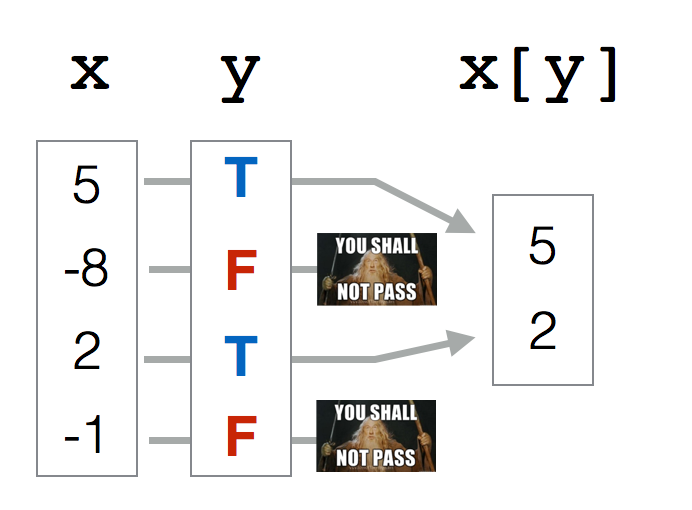
\includegraphics[width=500px]{images/indexgandolf} 

}

\caption{FALSE values in a logical vector are like lots of mini-Gandolfs. In this example, I am indexing a vector   exttt{x} with a logical vector y (y for example could be x > 0, so all positive values of x are TRUE and all negative values are FALSE). The result is a vector of length 2, which are the values of x for which the logical vector y was true. Gandolf stopped all the values of x for which y was FALSE.}\label{fig:unnamed-chunk-136}
\end{figure}

You could create logical vectors directly using \texttt{c()}. For
example, I could access every other value of the following vector as
follows:

\begin{Shaded}
\begin{Highlighting}[]
\NormalTok{a <-}\StringTok{ }\KeywordTok{c}\NormalTok{(}\DecValTok{1}\NormalTok{, }\DecValTok{2}\NormalTok{, }\DecValTok{3}\NormalTok{, }\DecValTok{4}\NormalTok{, }\DecValTok{5}\NormalTok{)}
\NormalTok{a[}\KeywordTok{c}\NormalTok{(}\OtherTok{TRUE}\NormalTok{, }\OtherTok{FALSE}\NormalTok{, }\OtherTok{TRUE}\NormalTok{, }\OtherTok{FALSE}\NormalTok{, }\OtherTok{TRUE}\NormalTok{)]}
\NormalTok{## [1] 1 3 5}
\end{Highlighting}
\end{Shaded}

As you can see, R returns all values of the vector \texttt{a} for which
the logical vector is TRUE.

\begin{figure}[htbp]
\centering
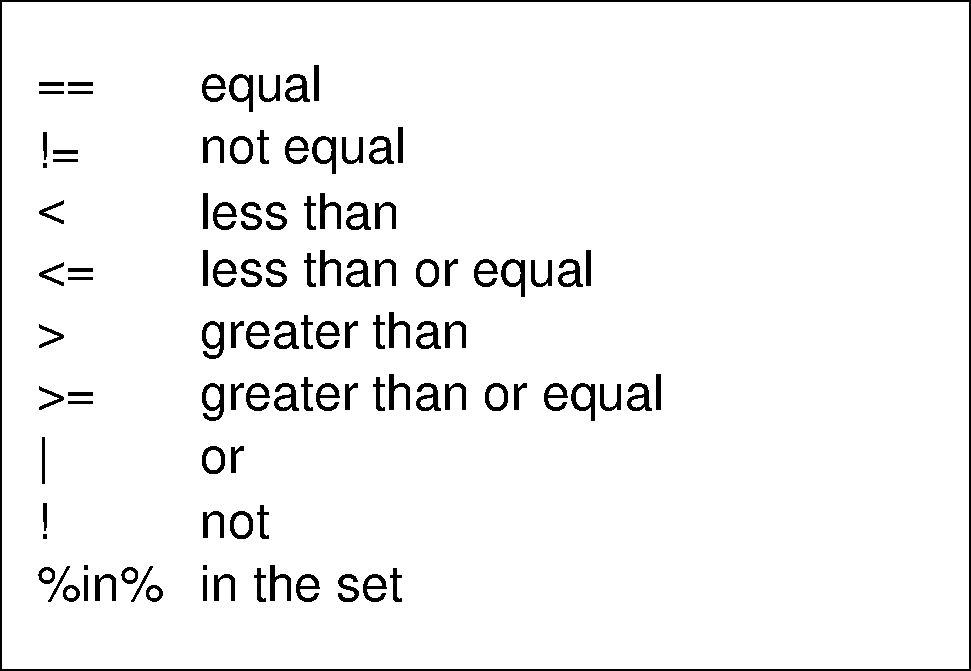
\includegraphics{YaRrr_files/figure-latex/unnamed-chunk-138-1.pdf}
\caption{\label{fig:unnamed-chunk-138}Logical comparison operators in R}
\end{figure}

However, creating logical vectors using \texttt{c()} is tedious.
Instead, it's better to create logical vectors from \emph{existing
vectors} using comparison operators like \textless{} (less than), ==
(equals to), and != (not equal to). A complete list of the most common
comparison operators is in Figure\textasciitilde{}\ref{fig:comparison}.
For example, let's create some logical vectors from our
\texttt{boat.ages} vector:

\begin{Shaded}
\begin{Highlighting}[]
\CommentTok{# Which ages are > 100?}
\NormalTok{boat.ages >}\StringTok{ }\DecValTok{100}
\NormalTok{##  [1]  TRUE FALSE  TRUE FALSE  TRUE FALSE  TRUE FALSE FALSE FALSE}

\CommentTok{# Which ages are equal to 23?}
\NormalTok{boat.ages ==}\StringTok{ }\DecValTok{23}
\NormalTok{##  [1] FALSE FALSE FALSE  TRUE FALSE FALSE FALSE FALSE FALSE FALSE}

\CommentTok{# Which boat names are equal to c?}
\NormalTok{boat.names ==}\StringTok{ "c"}
\NormalTok{##  [1] FALSE FALSE  TRUE FALSE FALSE FALSE FALSE FALSE FALSE FALSE}
\end{Highlighting}
\end{Shaded}

You can also create logical vectors by comparing a vector to another
vector of the same length. When you do this, R will compare values in
the same position (e.g.; the first values will be compared, then the
second values, etc.). For example, we can compare the \texttt{boat.cost}
and \texttt{boat.price} vectors to see which boats sold for a higher
price than their cost:

\begin{Shaded}
\begin{Highlighting}[]
\CommentTok{# Which boats had a higher price than cost?}
\NormalTok{boat.prices >}\StringTok{ }\NormalTok{boat.costs}
\NormalTok{##  [1]  TRUE  TRUE  TRUE FALSE  TRUE  TRUE  TRUE FALSE  TRUE  TRUE}

\CommentTok{# Which boats had a lower price than cost?}
\NormalTok{boat.prices <}\StringTok{ }\NormalTok{boat.costs}
\NormalTok{##  [1] FALSE FALSE FALSE  TRUE FALSE FALSE FALSE  TRUE FALSE FALSE}
\end{Highlighting}
\end{Shaded}

Once you've created a logical vector using a comparison operator, you
can use it to index any vector with the same length. Here, I'll use
logical vectors to get the prices of boats whose ages were greater than
100:

\begin{Shaded}
\begin{Highlighting}[]
\CommentTok{# What were the prices of boats older than 100?}
\NormalTok{boat.prices[boat.ages >}\StringTok{ }\DecValTok{100}\NormalTok{]}
\NormalTok{## [1]  53  54 264 532}
\end{Highlighting}
\end{Shaded}

Here's how logical indexing works step-by-step:

\begin{Shaded}
\begin{Highlighting}[]
\CommentTok{# Which boat prices are greater than 100?}
\NormalTok{boat.ages >}\StringTok{ }\DecValTok{100}
\NormalTok{##  [1]  TRUE FALSE  TRUE FALSE  TRUE FALSE  TRUE FALSE FALSE FALSE}

\CommentTok{# Writing the logical index by hand (you'd never do this!)}
\NormalTok{boat.prices[}\KeywordTok{c}\NormalTok{(}\OtherTok{TRUE}\NormalTok{, }\OtherTok{FALSE}\NormalTok{, }\OtherTok{TRUE}\NormalTok{, }\OtherTok{FALSE}\NormalTok{, }\OtherTok{TRUE}\NormalTok{, }\OtherTok{FALSE}\NormalTok{, }\OtherTok{TRUE}\NormalTok{, }\OtherTok{FALSE}\NormalTok{, }\OtherTok{FALSE}\NormalTok{, }\OtherTok{FALSE}\NormalTok{)]}
\NormalTok{## [1]  53  54 264 532}

\CommentTok{# Doing it all in one step! You get the same answer}
\NormalTok{boat.prices[boat.ages >}\StringTok{ }\DecValTok{100}\NormalTok{]}
\NormalTok{## [1]  53  54 264 532}
\end{Highlighting}
\end{Shaded}

\subsection{\texorpdfstring{\texttt{\&} (and), \texttt{\textbar{}} (or),
\texttt{\%in\%}}{\& (and), \textbar{} (or), \%in\%}}\label{and-or-in}

In addition to using single comparison operators, you can combine
multiple logical vectors using the OR (which looks like
\texttt{\textbar{}} and AND \texttt{\textbackslash{}\&} commands. The OR
\texttt{\textbar{}} operation will return TRUE if any of the logical
vectors is TRUE, while the AND \texttt{\&} operation will only return
TRUE if all of the values in the logical vectors is TRUE. This is
especially powerful when you want to create a logical vector based on
criteria from multiple vectors.

For example, let's create a logical vector indicating which boats had a
price greater than 200 OR less than 100, and then use that vector to see
what the names of these boats were:

\begin{Shaded}
\begin{Highlighting}[]
\CommentTok{# Which boats had prices greater than 400 OR less than 100?}
\NormalTok{boat.prices >}\StringTok{ }\DecValTok{200} \NormalTok{|}\StringTok{ }\NormalTok{boat.prices <}\StringTok{ }\DecValTok{100}
\NormalTok{##  [1]  TRUE  TRUE  TRUE  TRUE  TRUE  TRUE  TRUE  TRUE  TRUE FALSE}

\CommentTok{# What were the NAMES of these boats}
\NormalTok{boat.names[boat.prices >}\StringTok{ }\DecValTok{200} \NormalTok{|}\StringTok{ }\NormalTok{boat.prices <}\StringTok{ }\DecValTok{100}\NormalTok{]}
\NormalTok{## [1] "a" "b" "c" "d" "e" "f" "g" "h" "i"}
\end{Highlighting}
\end{Shaded}

You can combine as many logical vectors as you want (as long as they all
have the same length!):

\begin{Shaded}
\begin{Highlighting}[]
\CommentTok{# Boat names of boats with a color of black OR with a price > 100}
\NormalTok{boat.names[boat.colors ==}\StringTok{ "black"} \NormalTok{|}\StringTok{ }\NormalTok{boat.prices >}\StringTok{ }\DecValTok{100}\NormalTok{]}
\NormalTok{## [1] "a" "e" "g" "i" "j"}

\CommentTok{# Names of blue boats with a price greater than 200}
\NormalTok{boat.names[boat.colors ==}\StringTok{ "blue"} \NormalTok{&}\StringTok{ }\NormalTok{boat.prices >}\StringTok{ }\DecValTok{200}\NormalTok{]}
\NormalTok{## [1] "e"}
\end{Highlighting}
\end{Shaded}

You can combine as many logical vectors as you want to create
increasingly complex selection criteria. For example, the following
logical vector returns TRUE for cases where the boat colors are black OR
brown, AND where the price was not equal to 100:

\begin{Shaded}
\begin{Highlighting}[]
\CommentTok{# Which boats were eithe black or brown, AND had a price less than 100?}
\NormalTok{(boat.colors ==}\StringTok{ "black"} \NormalTok{|}\StringTok{ }\NormalTok{boat.colors ==}\StringTok{ "brown"}\NormalTok{) &}\StringTok{ }\NormalTok{boat.prices <}\StringTok{ }\DecValTok{100}
\NormalTok{##  [1]  TRUE FALSE FALSE FALSE FALSE FALSE FALSE FALSE  TRUE FALSE}

\CommentTok{# What were the names of these boats?}
\NormalTok{boat.names[(boat.colors ==}\StringTok{ "black"} \NormalTok{|}\StringTok{ }\NormalTok{boat.colors ==}\StringTok{ "brown"}\NormalTok{) &}\StringTok{ }\NormalTok{boat.prices <}\StringTok{ }\DecValTok{100}\NormalTok{]}
\NormalTok{## [1] "a" "i"}
\end{Highlighting}
\end{Shaded}

When using multiple criteria, make sure to use parentheses when
appropriate. If I didn't use parentheses above, I would get a different
answer.

The \texttt{\%in\%} operation helps you to easily create multiple OR
arguments.Imagine you have a vector of categorical data that can take on
many different values. For example, you could have a vector x indicating
people's favorite letters.

\begin{Shaded}
\begin{Highlighting}[]
\NormalTok{x <-}\StringTok{ }\KeywordTok{c}\NormalTok{(}\StringTok{"a"}\NormalTok{, }\StringTok{"t"}\NormalTok{, }\StringTok{"a"}\NormalTok{, }\StringTok{"b"}\NormalTok{, }\StringTok{"z"}\NormalTok{)}
\end{Highlighting}
\end{Shaded}

Now, let's say you want to create a logical vector indicating which
values are either a or b or c or d. You could create this logical vector
with multiple \textbar{} (OR) commands:

\begin{Shaded}
\begin{Highlighting}[]
\NormalTok{x ==}\StringTok{ "a"} \NormalTok{|}\StringTok{ }\NormalTok{x ==}\StringTok{ "b"} \NormalTok{|}\StringTok{ }\NormalTok{x ==}\StringTok{ "c"} \NormalTok{|}\StringTok{ }\NormalTok{x ==}\StringTok{ "d"}
\NormalTok{## [1]  TRUE FALSE  TRUE  TRUE FALSE}
\end{Highlighting}
\end{Shaded}

However, this takes a long time to write. Thankfully, the
\texttt{\%in\%} operation allows you to combine multiple OR comparisons
much faster. To use the \texttt{\%in\%} function, just put it in between
the original vector, and a new vector of possible values. The
\texttt{\%in\%} function goes through every value in the vector x, and
returns TRUE if it finds it in the vector of possible values --
otherwise it returns FALSE.

\begin{Shaded}
\begin{Highlighting}[]
\NormalTok{x %in%}\StringTok{ }\KeywordTok{c}\NormalTok{(}\StringTok{"a"}\NormalTok{, }\StringTok{"b"}\NormalTok{, }\StringTok{"c"}\NormalTok{, }\StringTok{"d"}\NormalTok{)}
\NormalTok{## [1]  TRUE FALSE  TRUE  TRUE FALSE}
\end{Highlighting}
\end{Shaded}

As you can see, the result is identical to our previous result.

\subsection{Counts and percentages from logical
vectors}\label{counts-and-percentages-from-logical-vectors}

Many (if not all) R functions will interpret TRUE values as 1 and FALSE
values as 0. This allows us to easily answer questions like ``How many
values in a data vector are greater than 0?'' or ``What percentage of
values are equal to 5?'' by applying the \texttt{sum()} or
\texttt{mean()} function to a logical vector.

We'll start with a vector x of length 10, containing 3 positive numbers
and 5 negative numbers.

\begin{Shaded}
\begin{Highlighting}[]
\NormalTok{x <-}\StringTok{ }\KeywordTok{c}\NormalTok{(}\DecValTok{1}\NormalTok{, }\DecValTok{2}\NormalTok{, }\DecValTok{3}\NormalTok{, -}\DecValTok{5}\NormalTok{, -}\DecValTok{5}\NormalTok{, -}\DecValTok{5}\NormalTok{, -}\DecValTok{5}\NormalTok{, -}\DecValTok{5}\NormalTok{)}
\end{Highlighting}
\end{Shaded}

We can create a logical vector to see which values are greater than 0:

\begin{Shaded}
\begin{Highlighting}[]
\NormalTok{x >}\StringTok{ }\DecValTok{0}
\NormalTok{## [1]  TRUE  TRUE  TRUE FALSE FALSE FALSE FALSE FALSE}
\end{Highlighting}
\end{Shaded}

Now, we'll use \texttt{sum()} and \texttt{mean()} on that logical vector
to see how many of the values in x are positive, and what percent are
positive. We should find that there are 5 TRUE values, and that 50\% of
the values (5 / 10) are TRUE.

\begin{Shaded}
\begin{Highlighting}[]
\KeywordTok{sum}\NormalTok{(x >}\StringTok{ }\DecValTok{0}\NormalTok{)}
\NormalTok{## [1] 3}
\KeywordTok{mean}\NormalTok{(x >}\StringTok{ }\DecValTok{0}\NormalTok{)}
\NormalTok{## [1] 0.38}
\end{Highlighting}
\end{Shaded}

This is a \emph{really} powerful tool. Pretty much \emph{any} time you
want to answer a question like ``How many of X are Y'' or ``What percent
of X are Y'', you use \texttt{sum()} or \texttt{mean()} function with a
logical vector as an argument.

\subsection{Additional Logical
functions}\label{additional-logical-functions}

R has lots of special functions that take vectors as arguments, and
return logical vectors based on multiple criteria. For example, you can
use the \texttt{is.na()} function to test which values of a vector are
missing. Table \ref{tab:logicalfunctions} contains some that I
frequently use:

\begin{longtable}[]{@{}llll@{}}
\caption{\label{tab:logicalfunctions} Functions to create and use logical
vectors.}\tabularnewline
\toprule
\begin{minipage}[b]{0.20\columnwidth}\raggedright\strut
Function\strut
\end{minipage} & \begin{minipage}[b]{0.23\columnwidth}\raggedright\strut
Description\strut
\end{minipage} & \begin{minipage}[b]{0.31\columnwidth}\raggedright\strut
Example\strut
\end{minipage} & \begin{minipage}[b]{0.06\columnwidth}\raggedright\strut
Result\strut
\end{minipage}\tabularnewline
\midrule
\endfirsthead
\toprule
\begin{minipage}[b]{0.20\columnwidth}\raggedright\strut
Function\strut
\end{minipage} & \begin{minipage}[b]{0.23\columnwidth}\raggedright\strut
Description\strut
\end{minipage} & \begin{minipage}[b]{0.31\columnwidth}\raggedright\strut
Example\strut
\end{minipage} & \begin{minipage}[b]{0.06\columnwidth}\raggedright\strut
Result\strut
\end{minipage}\tabularnewline
\midrule
\endhead
\begin{minipage}[t]{0.20\columnwidth}\raggedright\strut
\texttt{is.na(x)}\strut
\end{minipage} & \begin{minipage}[t]{0.23\columnwidth}\raggedright\strut
Which values in x are NA?\strut
\end{minipage} & \begin{minipage}[t]{0.31\columnwidth}\raggedright\strut
\texttt{is.na(c(2,\ NA,\ 5))}\strut
\end{minipage} & \begin{minipage}[t]{0.06\columnwidth}\raggedright\strut
FALSE, TRUE, FALSE\strut
\end{minipage}\tabularnewline
\begin{minipage}[t]{0.20\columnwidth}\raggedright\strut
\texttt{is.finite(x)}\strut
\end{minipage} & \begin{minipage}[t]{0.23\columnwidth}\raggedright\strut
Which values in x are numbers?\strut
\end{minipage} & \begin{minipage}[t]{0.31\columnwidth}\raggedright\strut
\texttt{is.finite(c(NA,\ 89,\ 0))}\strut
\end{minipage} & \begin{minipage}[t]{0.06\columnwidth}\raggedright\strut
FALSE, TRUE, TRUE\strut
\end{minipage}\tabularnewline
\begin{minipage}[t]{0.20\columnwidth}\raggedright\strut
\texttt{duplicated(x)}\strut
\end{minipage} & \begin{minipage}[t]{0.23\columnwidth}\raggedright\strut
Which values in x are duplicated?\strut
\end{minipage} & \begin{minipage}[t]{0.31\columnwidth}\raggedright\strut
\texttt{duplicated(c(1,\ 4,\ 1,\ 2))}\strut
\end{minipage} & \begin{minipage}[t]{0.06\columnwidth}\raggedright\strut
FALSE, FALSE, TRUE, FALSE\strut
\end{minipage}\tabularnewline
\begin{minipage}[t]{0.20\columnwidth}\raggedright\strut
\texttt{which(x)}\strut
\end{minipage} & \begin{minipage}[t]{0.23\columnwidth}\raggedright\strut
Which values in x are TRUE?\strut
\end{minipage} & \begin{minipage}[t]{0.31\columnwidth}\raggedright\strut
\texttt{which(c(TRUE,\ FALSE,\ TRUE))}\strut
\end{minipage} & \begin{minipage}[t]{0.06\columnwidth}\raggedright\strut
1, 3\strut
\end{minipage}\tabularnewline
\bottomrule
\end{longtable}

Logical vectors aren't just good for indexing, you can also use them to
figure out which values in a vector satisfy some criteria. To do this,
use the function \texttt{which()}. If you apply the function
\texttt{which()} to a logical vector, R will tell you which values of
the index are TRUE. For example:

\begin{Shaded}
\begin{Highlighting}[]
\CommentTok{# A vector of sex information}
\NormalTok{sex <-}\StringTok{ }\KeywordTok{c}\NormalTok{(}\StringTok{"m"}\NormalTok{, }\StringTok{"m"}\NormalTok{, }\StringTok{"f"}\NormalTok{, }\StringTok{"m"}\NormalTok{, }\StringTok{"f"}\NormalTok{, }\StringTok{"f"}\NormalTok{)}

\CommentTok{# Which values of sex are m?}
\KeywordTok{which}\NormalTok{(sex ==}\StringTok{ "m"}\NormalTok{)}
\NormalTok{## [1] 1 2 4}

\CommentTok{# Which values of sex are f?}
\KeywordTok{which}\NormalTok{(sex ==}\StringTok{ "f"}\NormalTok{)}
\NormalTok{## [1] 3 5 6}
\end{Highlighting}
\end{Shaded}

\section{Changing values of a vector}\label{changing-values-of-a-vector}

Now that you know how to index a vector, you can easily change specific
values in a vector using the assignment (\texttt{\textless{}-})
operation. To do this, just assign a vector of new values to the indexed
values of the original vector:

Let's create a vector \texttt{a} which contains 10 1s:

\begin{Shaded}
\begin{Highlighting}[]
\NormalTok{a <-}\StringTok{ }\KeywordTok{rep}\NormalTok{(}\DecValTok{1}\NormalTok{, }\DecValTok{10}\NormalTok{)}
\end{Highlighting}
\end{Shaded}

Now, let's change the first 5 values in the vector to 9s by indexing the
first five values, and assigning the value of 9:

\begin{Shaded}
\begin{Highlighting}[]
\NormalTok{a[}\DecValTok{1}\NormalTok{:}\DecValTok{5}\NormalTok{] <-}\StringTok{ }\DecValTok{9}
\NormalTok{a}
\NormalTok{##  [1] 9 9 9 9 9 1 1 1 1 1}
\end{Highlighting}
\end{Shaded}

Now let's change the last 5 values to 0s. We'll index the values 6
through 10, and assign a value of 0.

\begin{Shaded}
\begin{Highlighting}[]
\NormalTok{a[}\DecValTok{6}\NormalTok{:}\DecValTok{10}\NormalTok{] <-}\StringTok{ }\DecValTok{0}
\NormalTok{a}
\NormalTok{##  [1] 9 9 9 9 9 0 0 0 0 0}
\end{Highlighting}
\end{Shaded}

Of course, you can also change values of a vector using a logical
indexing vector. For example, let's say you have a vector of numbers
that should be from 1 to 10. If values are outside of this range, you
want to set them to either the minimum (1) or maximum (10) value:

\begin{Shaded}
\begin{Highlighting}[]
\CommentTok{# x is a vector of numbers that should be from 1 to 10}
\NormalTok{x <-}\StringTok{ }\KeywordTok{c}\NormalTok{(}\DecValTok{5}\NormalTok{, -}\DecValTok{5}\NormalTok{, }\DecValTok{7}\NormalTok{, }\DecValTok{4}\NormalTok{, }\DecValTok{11}\NormalTok{, }\DecValTok{5}\NormalTok{, -}\DecValTok{2}\NormalTok{)}

\CommentTok{# Assign values less than 1 to 1}
\NormalTok{x[x <}\StringTok{ }\DecValTok{1}\NormalTok{] <-}\StringTok{ }\DecValTok{1}

\CommentTok{# Assign values greater than 10 to 10}
\NormalTok{x[x >}\StringTok{ }\DecValTok{10}\NormalTok{] <-}\StringTok{ }\DecValTok{10}

\CommentTok{# Print the result!}
\NormalTok{x}
\NormalTok{## [1]  5  1  7  4 10  5  1}
\end{Highlighting}
\end{Shaded}

As you can see, our new values of x are now never less than 1 or greater
than 10!

\textbf{A note on indexing\ldots{}}

Technically, when you assign new values to a vector, you should always
assign a vector of the same length as the number of values that you are
updating. For example, given a vector a with 10 1s:

\begin{Shaded}
\begin{Highlighting}[]
\NormalTok{a <-}\StringTok{ }\KeywordTok{rep}\NormalTok{(}\DecValTok{1}\NormalTok{, }\DecValTok{10}\NormalTok{)}
\end{Highlighting}
\end{Shaded}

To update the first 5 values with 5 9s, we should assign a new vector of
5 9s

\begin{Shaded}
\begin{Highlighting}[]
\NormalTok{a[}\DecValTok{1}\NormalTok{:}\DecValTok{5}\NormalTok{] <-}\StringTok{ }\KeywordTok{c}\NormalTok{(}\DecValTok{9}\NormalTok{, }\DecValTok{9}\NormalTok{, }\DecValTok{9}\NormalTok{, }\DecValTok{9}\NormalTok{, }\DecValTok{9}\NormalTok{)}
\NormalTok{a}
\NormalTok{##  [1] 9 9 9 9 9 1 1 1 1 1}
\end{Highlighting}
\end{Shaded}

However, if we repeat this code but just assign a single 9, R will
repeat the value as many times as necessary to fill the indexed value of
the vector. That's why the following code still works:

\begin{Shaded}
\begin{Highlighting}[]
\NormalTok{a[}\DecValTok{1}\NormalTok{:}\DecValTok{5}\NormalTok{] <-}\StringTok{ }\DecValTok{9}
\NormalTok{a}
\NormalTok{##  [1] 9 9 9 9 9 1 1 1 1 1}
\end{Highlighting}
\end{Shaded}

In other languages this code wouldn't work because we're trying to
replace 5 values with just 1. However, this is a case where R bends the
rules a bit.

\subsection{Ex: Fixing invalid responses to a Happiness
survey}\label{ex-fixing-invalid-responses-to-a-happiness-survey}

\begin{figure}

{\centering 
\includegraphics[width=300px]{images/happiness} 

}

\end{figure}

Assigning and indexing is a particularly helpful tool when, for example,
you want to remove invalid values in a vector before performing an
analysis. For example, let's say you asked 10 people how happy they were
on a scale of 1 to 5 and received the following responses:

\begin{Shaded}
\begin{Highlighting}[]
\NormalTok{happy <-}\StringTok{ }\KeywordTok{c}\NormalTok{(}\DecValTok{1}\NormalTok{, }\DecValTok{4}\NormalTok{, }\DecValTok{2}\NormalTok{, }\DecValTok{999}\NormalTok{, }\DecValTok{2}\NormalTok{, }\DecValTok{3}\NormalTok{, -}\DecValTok{2}\NormalTok{, }\DecValTok{3}\NormalTok{, }\DecValTok{2}\NormalTok{, }\DecValTok{999}\NormalTok{)}
\end{Highlighting}
\end{Shaded}

As you can see, we have some invalid values (999 and -2) in this vector.
To remove them, we'll use logical indexing to change the invalid values
(999 and -2) to NA. We'll create a logical vector indicating which
values of \texttt{happy} are \emph{invalid} using the \texttt{\%in\%}
operation. Because we want to see which values are \emph{invalid}, we'll
add the \texttt{==\ FALSE} condition (If we don't, the index will tell
us which values \emph{are} valid).

\begin{Shaded}
\begin{Highlighting}[]
\CommentTok{# Which values of happy are NOT in the set 1:5?}
\NormalTok{invalid <-}\StringTok{ }\NormalTok{(happy %in%}\StringTok{ }\DecValTok{1}\NormalTok{:}\DecValTok{5}\NormalTok{) ==}\StringTok{ }\OtherTok{FALSE}
\NormalTok{invalid}
\NormalTok{##  [1] FALSE FALSE FALSE  TRUE FALSE FALSE  TRUE FALSE FALSE  TRUE}
\end{Highlighting}
\end{Shaded}

Now that we have a logical index \texttt{invalid} telling us which
values are invalid (that is, not in the set 1 through 5), we'll index
\texttt{happy} with \texttt{invalid}, and assign the invalid values as
NA:

\begin{Shaded}
\begin{Highlighting}[]
\CommentTok{# Convert any invalid values in happy to NA}
\NormalTok{happy[invalid] <-}\StringTok{ }\OtherTok{NA}
\NormalTok{happy}
\NormalTok{##  [1]  1  4  2 NA  2  3 NA  3  2 NA}
\end{Highlighting}
\end{Shaded}

We can also recode all the invalid values of \textt{happy} in one line
as follows:

\begin{Shaded}
\begin{Highlighting}[]
\CommentTok{# Convert all values of happy that are NOT integers from 1 to 5 to NA}
\NormalTok{happy[(happy %in%}\StringTok{ }\DecValTok{1}\NormalTok{:}\DecValTok{5}\NormalTok{) ==}\StringTok{ }\OtherTok{FALSE}\NormalTok{] <-}\StringTok{ }\OtherTok{NA}
\end{Highlighting}
\end{Shaded}

As you can see, \texttt{happy} now has NAs for previously invalid
values. Now we can take a \texttt{mean()} of the vector and see the mean
of the valid responses.

\begin{Shaded}
\begin{Highlighting}[]
\CommentTok{# Include na.rm = TRUE to ignore NA values}
\KeywordTok{mean}\NormalTok{(happy, }\DataTypeTok{na.rm =} \OtherTok{TRUE}\NormalTok{)}
\NormalTok{## [1] 2.4}
\end{Highlighting}
\end{Shaded}

\section{Test your R Might!: Movie
data}\label{test-your-r-might-movie-data}

\begin{figure}

{\centering 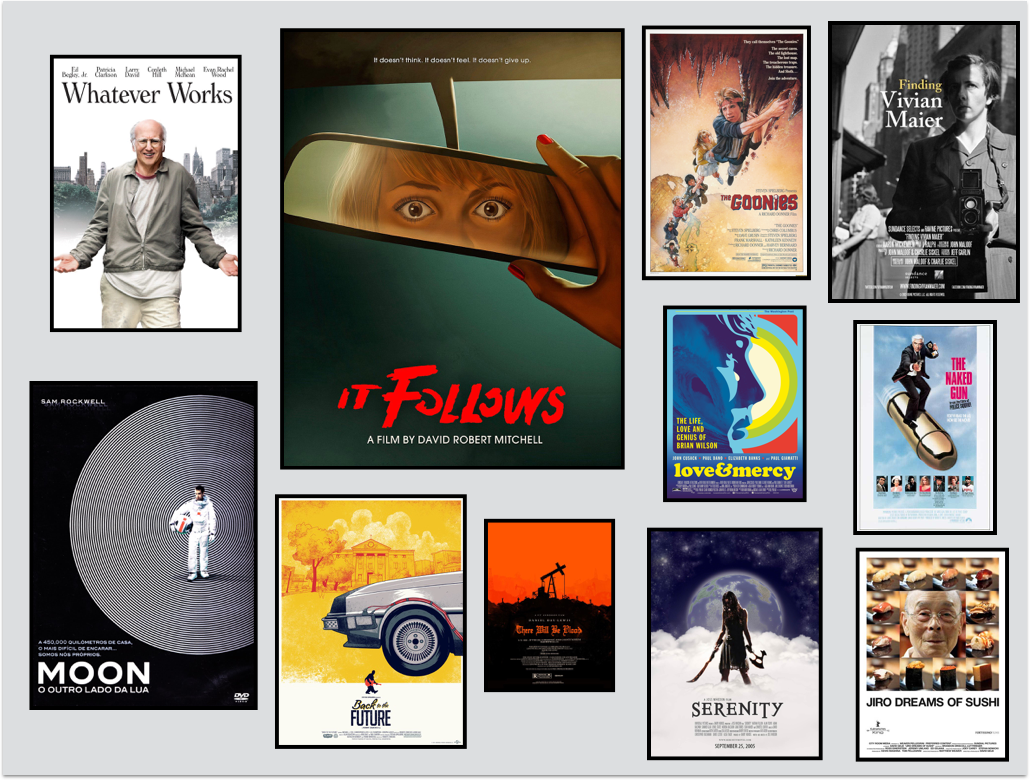
\includegraphics[width=600px]{images/moviecollage} 

}

\end{figure}

Table \ref{tab:moviedata} contains data about 10 of my favorite movies.

\begin{table}

\caption{\label{tab:moviedata}Some of my favorite movies}
\centering
\begin{tabular}[t]{l|r|r|l|r|l}
\hline
movie & year & boxoffice & genre & time & rating\\
\hline
Whatever Works & 2009 & 35.0 & Comedy & 92 & PG-13\\
\hline
It Follows & 2015 & 15.0 & Horror & 97 & R\\
\hline
Love and Mercy & 2015 & 15.0 & Drama & 120 & R\\
\hline
The Goonies & 1985 & 62.0 & Adventure & 90 & PG\\
\hline
Jiro Dreams of Sushi & 2012 & 3.0 & Documentary & 81 & G\\
\hline
There Will be Blood & 2007 & 10.0 & Drama & 158 & R\\
\hline
Moon & 2009 & 321.0 & Science Fiction & 97 & R\\
\hline
Spice World & 1988 & 79.0 & Comedy & -84 & PG-13\\
\hline
Serenity & 2005 & 39.0 & Science Fiction & 119 & PG-13\\
\hline
Finding Vivian Maier & 2014 & 1.5 & Documentary & 84 & Unrated\\
\hline
\end{tabular}
\end{table}

\begin{enumerate}
\def\labelenumi{\arabic{enumi}.}
\setcounter{enumi}{-1}
\item
  Create new data vectors for each column.
\item
  What is the name of the 10th movie in the list?
\item
  What are the genres of the first 4 movies?
\item
  Some joker put Spice World in the movie names -- it should be ``The
  Naked Gun'' Please correct the name.
\item
  What were the names of the movies made before 1990?
\item
  How many movies were Dramas? What percent of the 10 movies were
  Dramas?
\item
  One of the values in the \texttt{time} vector is invalid. Convert any
  invalid values in this vector to NA. Then, calculate the mean movie
  time
\item
  What were the names of the Comedy movies? What were their boxoffice
  totals? (Two separate questions)
\item
  What were the names of the movies that made less than \$50 Million
  dollars AND were Comedies?
\item
  What was the median boxoffice revenue of movies rated either G or PG?
\item
  What percent of the movies were rated R OR were comedies?
\end{enumerate}

\chapter{Matrices and Dataframes}\label{matricesdataframes}

\begin{figure}

{\centering 
\includegraphics[width=300px]{images/matrix} 

}

\caption{Did you actually think I could talk about matrices without a Matrix reference?!}\label{fig:unnamed-chunk-168}
\end{figure}

\section{What are matrices and
dataframes?}\label{what-are-matrices-and-dataframes}

By now, you should be comfortable with scalar and vector objects.
However, you may have noticed that neither object types are appropriate
for storing lots of data -- such as the results of a survey or
experiment. Thankfully, R has two object types that represent large data
structures much better: \textbf{matrices} and **dataframes*\}**.

Matrices and dataframes are very similar to spreadsheets in Excel or
data files in SPSS. Every matrix or dataframe contains rows (call that
number m) and columns (n). Thus, wile a vector has 1 dimension (its
length), matrices and dataframes both have 2-dimensions -- representing
their width and height. You can think of a matrix or dataframe as a
combination of \texttt{n} vectors, where each vector has a length of
\texttt{m}. See Figure \ref{fig:scalervectormatrix} to see the shocking
difference between these data objects.

\begin{figure}[htbp]
\centering
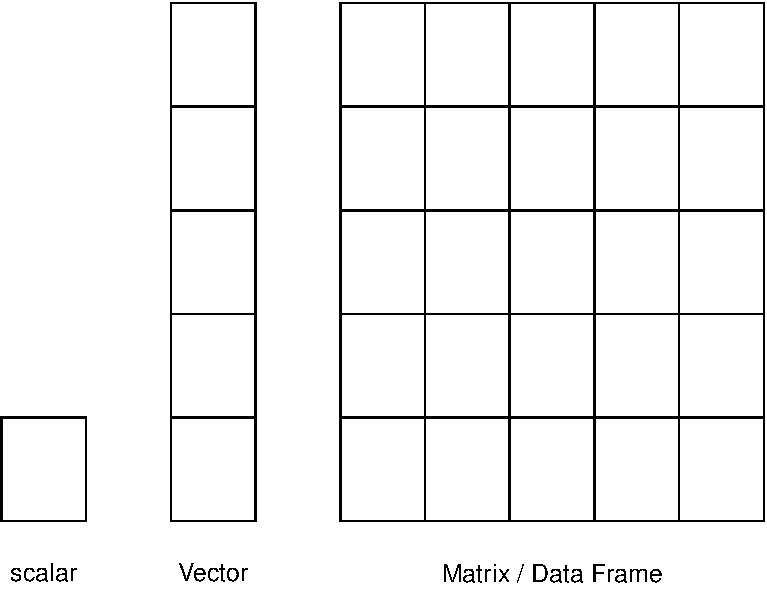
\includegraphics{YaRrr_files/figure-latex/scalervectormatrix-1.pdf}
\caption{\label{fig:scalervectormatrix}scalar, Vector, Matrix\ldots{}
::drops mike::}
\end{figure}

While matrices and dataframes look very similar, they aren't exactly the
same. While a matrix can contain \emph{either} character \emph{or}
numeric columns, a dataframe can contain \emph{both} numeric and
character columns. Because dataframes are more flexible, most real-world
datasets, such as surveys containing both numeric (e.g.; age, response
times) and character (e.g.; sex, favorite movie) data, will be stored as
dataframes in R.

\textbf{WTF} -- If dataframes are more flexible than matrices, why do we
use matrices at all? The answer is that, because they are simpler,
matrices take up less computational space than dataframes. Additionally,
some functions require matrices as inputs to ensure that they work
correctly.

In the next section, we'll cover the most common functions for creating
matrix and dataframe objects. We'll then move on to functions that take
matrices and dataframes as inputs.

\section{Creating matrices and
dataframes}\label{creating-matrices-and-dataframes}

There are a number of ways to create your own matrix and dataframe
objects in R. The most common functions are presented in Table
\ref{tab:matrixfunctions}. Because matrices and dataframes are just
combinations of vectors, each function takes one or more vectors as
inputs, and returns a matrix or a dataframe.

\begin{longtable}[]{@{}lll@{}}
\caption{\label{tab:matrixfunctions} Functions to create matrices and
dataframes.}\tabularnewline
\toprule
\begin{minipage}[b]{0.19\columnwidth}\raggedright\strut
Function\strut
\end{minipage} & \begin{minipage}[b]{0.27\columnwidth}\raggedright\strut
Description\strut
\end{minipage} & \begin{minipage}[b]{0.41\columnwidth}\raggedright\strut
Example\strut
\end{minipage}\tabularnewline
\midrule
\endfirsthead
\toprule
\begin{minipage}[b]{0.19\columnwidth}\raggedright\strut
Function\strut
\end{minipage} & \begin{minipage}[b]{0.27\columnwidth}\raggedright\strut
Description\strut
\end{minipage} & \begin{minipage}[b]{0.41\columnwidth}\raggedright\strut
Example\strut
\end{minipage}\tabularnewline
\midrule
\endhead
\begin{minipage}[t]{0.19\columnwidth}\raggedright\strut
\texttt{cbind(a,\ b,\ c)}\strut
\end{minipage} & \begin{minipage}[t]{0.27\columnwidth}\raggedright\strut
Combine vectors as columns in a matrix\strut
\end{minipage} & \begin{minipage}[t]{0.41\columnwidth}\raggedright\strut
\texttt{cbind(1:5,\ 6:10,\ 11:15)}\strut
\end{minipage}\tabularnewline
\begin{minipage}[t]{0.19\columnwidth}\raggedright\strut
\texttt{rbind(a,\ b,\ c)}\strut
\end{minipage} & \begin{minipage}[t]{0.27\columnwidth}\raggedright\strut
Combine vectors as rows in a matrix\strut
\end{minipage} & \begin{minipage}[t]{0.41\columnwidth}\raggedright\strut
\texttt{rbind(1:5,\ 6:10,\ 11:15)}\strut
\end{minipage}\tabularnewline
\begin{minipage}[t]{0.19\columnwidth}\raggedright\strut
\texttt{matrix(x,\ nrow,\ ncol,\ byrow)}\strut
\end{minipage} & \begin{minipage}[t]{0.27\columnwidth}\raggedright\strut
Create a matrix from a vector \texttt{x}\strut
\end{minipage} & \begin{minipage}[t]{0.41\columnwidth}\raggedright\strut
\texttt{matrix(x\ =\ 1:12,\ nrow\ =\ 3,\ ncol\ =\ 4)}\strut
\end{minipage}\tabularnewline
\begin{minipage}[t]{0.19\columnwidth}\raggedright\strut
\texttt{data.frame()}\strut
\end{minipage} & \begin{minipage}[t]{0.27\columnwidth}\raggedright\strut
Create a dataframe from named columns\strut
\end{minipage} & \begin{minipage}[t]{0.41\columnwidth}\raggedright\strut
\texttt{data.frame("age"\ =\ c(19,\ 21),}
\texttt{sex\ =\ c("m",\ "f"))}\strut
\end{minipage}\tabularnewline
\bottomrule
\end{longtable}

\subsection{\texorpdfstring{\texttt{cbind()},
\texttt{rbind()}}{cbind(), rbind()}}\label{cbind-rbind}

\texttt{cbind()} and \texttt{rbind()} both create matrices by combining
several vectors of the same length. \texttt{cbind()} combines vectors as
columns, while \texttt{rbind()} combines them as rows.

Let's use these functions to create a matrix with the numbers 1 through
30. First, we'll create three vectors of length 10, then we'll combine
them into one matrix. As you will see, the \texttt{cbind()} function
will combine the vectors as columns in the final matrix, while the
\texttt{rbind()} function will combine them as rows.

\begin{Shaded}
\begin{Highlighting}[]
\NormalTok{x <-}\StringTok{ }\DecValTok{1}\NormalTok{:}\DecValTok{5}
\NormalTok{y <-}\StringTok{ }\DecValTok{6}\NormalTok{:}\DecValTok{10}
\NormalTok{z <-}\StringTok{ }\DecValTok{11}\NormalTok{:}\DecValTok{15}

\CommentTok{# Create a matrix where x, y and z are columns}
\KeywordTok{cbind}\NormalTok{(x, y, z)}
\NormalTok{##      x  y  z}
\NormalTok{## [1,] 1  6 11}
\NormalTok{## [2,] 2  7 12}
\NormalTok{## [3,] 3  8 13}
\NormalTok{## [4,] 4  9 14}
\NormalTok{## [5,] 5 10 15}

\CommentTok{# Create a matrix where x, y and z are rows}
\KeywordTok{rbind}\NormalTok{(x, y, z)}
\NormalTok{##   [,1] [,2] [,3] [,4] [,5]}
\NormalTok{## x    1    2    3    4    5}
\NormalTok{## y    6    7    8    9   10}
\NormalTok{## z   11   12   13   14   15}
\end{Highlighting}
\end{Shaded}

\subsection{\texorpdfstring{\texttt{matrix()}}{matrix()}}\label{matrix}

\textbf{Remember}: Matrices can either contain numbers \emph{or}
character vectors, not both!. If you try to create a matrix with both
numbers and characters, it will turn all the numbers into characters:

\begin{Shaded}
\begin{Highlighting}[]
\CommentTok{# Creating a matrix with numeric and character columns will make everything a character:}

\KeywordTok{cbind}\NormalTok{(}\KeywordTok{c}\NormalTok{(}\DecValTok{1}\NormalTok{, }\DecValTok{2}\NormalTok{, }\DecValTok{3}\NormalTok{, }\DecValTok{4}\NormalTok{, }\DecValTok{5}\NormalTok{),}
      \KeywordTok{c}\NormalTok{(}\StringTok{"a"}\NormalTok{, }\StringTok{"b"}\NormalTok{, }\StringTok{"c"}\NormalTok{, }\StringTok{"d"}\NormalTok{, }\StringTok{"e"}\NormalTok{))}
\NormalTok{##      [,1] [,2]}
\NormalTok{## [1,] "1"  "a" }
\NormalTok{## [2,] "2"  "b" }
\NormalTok{## [3,] "3"  "c" }
\NormalTok{## [4,] "4"  "d" }
\NormalTok{## [5,] "5"  "e"}
\end{Highlighting}
\end{Shaded}

The \texttt{matrix()} function creates a matrix form a single vector of
data. The function has 3 main inputs: \texttt{data} -- a vector of data,
\texttt{nrow} -- the number of rows you want in the matrix, and
\texttt{ncol} -- the number of columns you want in the matrix, and
\texttt{byrow} -- a logical value indicating whether you want to fill
the matrix by rows. Check out the help menu for the matrix function
(`?matrix) to see some additional inputs.

Let's use the \texttt{matrix()} function to re-create a matrix
containing the values from 1 to 10.

\begin{Shaded}
\begin{Highlighting}[]
\CommentTok{# Create a matrix of the integers 1:10,}
\CommentTok{#  with 5 rows and 2 columns}

\KeywordTok{matrix}\NormalTok{(}\DataTypeTok{data =} \DecValTok{1}\NormalTok{:}\DecValTok{10}\NormalTok{,}
       \DataTypeTok{nrow =} \DecValTok{5}\NormalTok{,}
       \DataTypeTok{ncol =} \DecValTok{2}\NormalTok{)}
\NormalTok{##      [,1] [,2]}
\NormalTok{## [1,]    1    6}
\NormalTok{## [2,]    2    7}
\NormalTok{## [3,]    3    8}
\NormalTok{## [4,]    4    9}
\NormalTok{## [5,]    5   10}

\CommentTok{# Now with 2 rows and 5 columns}
\KeywordTok{matrix}\NormalTok{(}\DataTypeTok{data =} \DecValTok{1}\NormalTok{:}\DecValTok{10}\NormalTok{,}
       \DataTypeTok{nrow =} \DecValTok{2}\NormalTok{,}
       \DataTypeTok{ncol =} \DecValTok{5}\NormalTok{)}
\NormalTok{##      [,1] [,2] [,3] [,4] [,5]}
\NormalTok{## [1,]    1    3    5    7    9}
\NormalTok{## [2,]    2    4    6    8   10}

\CommentTok{# Now with 2 rows and 5 columns, but fill by row instead of columns}
\KeywordTok{matrix}\NormalTok{(}\DataTypeTok{data =} \DecValTok{1}\NormalTok{:}\DecValTok{10}\NormalTok{,}
       \DataTypeTok{nrow =} \DecValTok{2}\NormalTok{,}
       \DataTypeTok{ncol =} \DecValTok{5}\NormalTok{,}
       \DataTypeTok{byrow =} \OtherTok{TRUE}\NormalTok{)}
\NormalTok{##      [,1] [,2] [,3] [,4] [,5]}
\NormalTok{## [1,]    1    2    3    4    5}
\NormalTok{## [2,]    6    7    8    9   10}
\end{Highlighting}
\end{Shaded}

\subsection{\texorpdfstring{\texttt{data.frame()}}{data.frame()}}\label{data.frame}

To create a dataframe from vectors, use the \texttt{data.frame()}
function. The \texttt{data.frame()} function works very similarly to
\texttt{cbind()} -- the only difference is that in \texttt{data.frame()}
you specify names to each of the columns as you define them. Again,
unlike matrices, dataframes can contain \emph{both} string vectors and
numeric vectors within the same object. Because they are more flexible
than matrices, most large datasets in R will be stored as dataframes.

Let's create a simple dataframe called \texttt{survey} using the
\texttt{data.frame()} function with a mixture of text and numeric
columns:

\begin{Shaded}
\begin{Highlighting}[]
\CommentTok{# Create a dataframe of survey data}

\NormalTok{survey <-}\StringTok{ }\KeywordTok{data.frame}\NormalTok{(}\StringTok{"index"} \NormalTok{=}\StringTok{ }\KeywordTok{c}\NormalTok{(}\DecValTok{1}\NormalTok{, }\DecValTok{2}\NormalTok{, }\DecValTok{3}\NormalTok{, }\DecValTok{4}\NormalTok{, }\DecValTok{5}\NormalTok{),}
                     \StringTok{"sex"} \NormalTok{=}\StringTok{ }\KeywordTok{c}\NormalTok{(}\StringTok{"m"}\NormalTok{, }\StringTok{"m"}\NormalTok{, }\StringTok{"m"}\NormalTok{, }\StringTok{"f"}\NormalTok{, }\StringTok{"f"}\NormalTok{),}
                     \StringTok{"age"} \NormalTok{=}\StringTok{ }\KeywordTok{c}\NormalTok{(}\DecValTok{99}\NormalTok{, }\DecValTok{46}\NormalTok{, }\DecValTok{23}\NormalTok{, }\DecValTok{54}\NormalTok{, }\DecValTok{23}\NormalTok{))}
\NormalTok{survey}
\NormalTok{##   index sex age}
\NormalTok{## 1     1   m  99}
\NormalTok{## 2     2   m  46}
\NormalTok{## 3     3   m  23}
\NormalTok{## 4     4   f  54}
\NormalTok{## 5     5   f  23}
\end{Highlighting}
\end{Shaded}

\subsubsection{\texorpdfstring{\texttt{stringsAsFactors\ =\ FALSE}}{stringsAsFactors = FALSE}}\label{stringsasfactors-false}

Thre is one key argument to \texttt{data.frame()} and similar functions
called \texttt{stringsAsFactors}. By default, the \texttt{data.frame()}
function will automctailly convert any string columns to a specific type
of object called a \textbf{factor} in R. A factor is nominal variable
that has a well-specified possible set of values that it can take on.
For example, one can create a factor \texttt{sex} that can \emph{only}
take on the values \texttt{"male"} and \texttt{"female"}.

However, as I'm sure you're discover, having R automatically convert
your string data to factors can lead to lots of strange results. For
example: if you have a factor of sex data, but then you want to add a
new value called \texttt{other}, R will yell at you and return an error.
I \emph{hate}, \emph{hate}, \emph{HATE} when this happens. While there
are very, very rare cases when I find factors use ful, I almost always
don't want or need them. For this reason, I avoid them at all costs.

To tell R to \emph{not} convert your string columns to factors, you need
to include the argument \texttt{stringsAsFactors\ =\ FALSE} when using
functions such as \texttt{data.frame()}

For example, let's look at the clases of the columns in the dataframe
\texttt{survey} that we just created using the \texttt{str()} function
(we'll go over this function in section XXX)

\begin{Shaded}
\begin{Highlighting}[]
\CommentTok{# Show me the structure of the survey dataframe}
\KeywordTok{str}\NormalTok{(survey)}
\NormalTok{## 'data.frame':    5 obs. of  3 variables:}
\NormalTok{##  $ index: num  1 2 3 4 5}
\NormalTok{##  $ sex  : Factor w/ 2 levels "f","m": 2 2 2 1 1}
\NormalTok{##  $ age  : num  99 46 23 54 23}
\end{Highlighting}
\end{Shaded}

AAAAA!!! R has converted the column \texttt{sex} to a factor with
\emph{only} two possible levels! This can cause major problems later!
Let's create the dataframe again using the argument
\texttt{stringsAsFactors\ =\ FALSE} to make sure that this doesn't
happen:

\begin{Shaded}
\begin{Highlighting}[]
\CommentTok{# Create a dataframe of survey data WITHOUT factors}
\NormalTok{survey <-}\StringTok{ }\KeywordTok{data.frame}\NormalTok{(}\StringTok{"index"} \NormalTok{=}\StringTok{ }\KeywordTok{c}\NormalTok{(}\DecValTok{1}\NormalTok{, }\DecValTok{2}\NormalTok{, }\DecValTok{3}\NormalTok{, }\DecValTok{4}\NormalTok{, }\DecValTok{5}\NormalTok{),}
                     \StringTok{"sex"} \NormalTok{=}\StringTok{ }\KeywordTok{c}\NormalTok{(}\StringTok{"m"}\NormalTok{, }\StringTok{"m"}\NormalTok{, }\StringTok{"m"}\NormalTok{, }\StringTok{"f"}\NormalTok{, }\StringTok{"f"}\NormalTok{),}
                     \StringTok{"age"} \NormalTok{=}\StringTok{ }\KeywordTok{c}\NormalTok{(}\DecValTok{99}\NormalTok{, }\DecValTok{46}\NormalTok{, }\DecValTok{23}\NormalTok{, }\DecValTok{54}\NormalTok{, }\DecValTok{23}\NormalTok{),}
                     \DataTypeTok{stringsAsFactors =} \OtherTok{FALSE}\NormalTok{)}
\end{Highlighting}
\end{Shaded}

Now let's look at the new version and make sure there are no factors:

\begin{Shaded}
\begin{Highlighting}[]
\CommentTok{# Print the result (it looks the same as before)}
\NormalTok{survey}
\NormalTok{##   index sex age}
\NormalTok{## 1     1   m  99}
\NormalTok{## 2     2   m  46}
\NormalTok{## 3     3   m  23}
\NormalTok{## 4     4   f  54}
\NormalTok{## 5     5   f  23}

\CommentTok{# Look at the structure: no more factors!}
\KeywordTok{str}\NormalTok{(survey)}
\NormalTok{## 'data.frame':    5 obs. of  3 variables:}
\NormalTok{##  $ index: num  1 2 3 4 5}
\NormalTok{##  $ sex  : chr  "m" "m" "m" "f" ...}
\NormalTok{##  $ age  : num  99 46 23 54 23}
\end{Highlighting}
\end{Shaded}

\subsection{Dataframes pre-loaded in
R}\label{dataframes-pre-loaded-in-r}

Now you know how to use functions like \texttt{cbind()} and
\texttt{data.frame()} to manually create your own matrices and
dataframes in R. However, for demonstration purposes, it's frequently
easier to use existing dataframes rather than always having to create
your own. Thankfully, R has us covered: R has several datasets that come
pre-installed in a package called \texttt{datasets} -- you don't need to
install this package, it's included in the base R software. While you
probably won't make any major scientific discoveries with these
datasets, they allow all R users to test and compare code on the same
sets of data. To see a complete list of all the datasets included in the
\texttt{datasets} package, run the code:
\texttt{library(help\ =\ "datasets")}. Table \ref{tab:datasets} shows a
few datasets that we will be using in future examples:

\begin{longtable}[]{@{}llll@{}}
\caption{\label{tab:datasets} A few datasets you can access in
R.}\tabularnewline
\toprule
\begin{minipage}[b]{0.16\columnwidth}\raggedright\strut
Dataset\strut
\end{minipage} & \begin{minipage}[b]{0.38\columnwidth}\raggedright\strut
Description\strut
\end{minipage} & \begin{minipage}[b]{0.07\columnwidth}\raggedright\strut
Rows\strut
\end{minipage} & \begin{minipage}[b]{0.09\columnwidth}\raggedright\strut
Columns\strut
\end{minipage}\tabularnewline
\midrule
\endfirsthead
\toprule
\begin{minipage}[b]{0.16\columnwidth}\raggedright\strut
Dataset\strut
\end{minipage} & \begin{minipage}[b]{0.38\columnwidth}\raggedright\strut
Description\strut
\end{minipage} & \begin{minipage}[b]{0.07\columnwidth}\raggedright\strut
Rows\strut
\end{minipage} & \begin{minipage}[b]{0.09\columnwidth}\raggedright\strut
Columns\strut
\end{minipage}\tabularnewline
\midrule
\endhead
\begin{minipage}[t]{0.16\columnwidth}\raggedright\strut
\texttt{ChickWeight}\strut
\end{minipage} & \begin{minipage}[t]{0.38\columnwidth}\raggedright\strut
Experiment on the effect of diet on early growth of chicks.\strut
\end{minipage} & \begin{minipage}[t]{0.07\columnwidth}\raggedright\strut
578\strut
\end{minipage} & \begin{minipage}[t]{0.09\columnwidth}\raggedright\strut
4\strut
\end{minipage}\tabularnewline
\begin{minipage}[t]{0.16\columnwidth}\raggedright\strut
\texttt{InsectSprays}\strut
\end{minipage} & \begin{minipage}[t]{0.38\columnwidth}\raggedright\strut
The counts of insects in agricultural experimental units treated with
different insecticides.\strut
\end{minipage} & \begin{minipage}[t]{0.07\columnwidth}\raggedright\strut
72\strut
\end{minipage} & \begin{minipage}[t]{0.09\columnwidth}\raggedright\strut
2\strut
\end{minipage}\tabularnewline
\begin{minipage}[t]{0.16\columnwidth}\raggedright\strut
\texttt{ToothGrowth}\strut
\end{minipage} & \begin{minipage}[t]{0.38\columnwidth}\raggedright\strut
Length of odontoblasts (cells responsible for tooth growth) in 60 guinea
pigs.\strut
\end{minipage} & \begin{minipage}[t]{0.07\columnwidth}\raggedright\strut
60\strut
\end{minipage} & \begin{minipage}[t]{0.09\columnwidth}\raggedright\strut
3\strut
\end{minipage}\tabularnewline
\begin{minipage}[t]{0.16\columnwidth}\raggedright\strut
\texttt{PlantGrowth}\strut
\end{minipage} & \begin{minipage}[t]{0.38\columnwidth}\raggedright\strut
Results from an experiment to compare yields (as measured by dried
weight of plants) obtained under a control and two different treatment
conditions.\strut
\end{minipage} & \begin{minipage}[t]{0.07\columnwidth}\raggedright\strut
30\strut
\end{minipage} & \begin{minipage}[t]{0.09\columnwidth}\raggedright\strut
2\strut
\end{minipage}\tabularnewline
\bottomrule
\end{longtable}

\section{Matrix and dataframe
functions}\label{matrix-and-dataframe-functions}

R has lots of functions for viewing matrices and dataframes and
returning information about them. Table \ref{tab:dataframefunctions}
shows some of the most common:

\begin{longtable}[]{@{}ll@{}}
\caption{\label{tab:dataframefunctions} Important functions for
understanding matrices and dataframes.}\tabularnewline
\toprule
\begin{minipage}[b]{0.34\columnwidth}\raggedright\strut
Function\strut
\end{minipage} & \begin{minipage}[b]{0.41\columnwidth}\raggedright\strut
Description\strut
\end{minipage}\tabularnewline
\midrule
\endfirsthead
\toprule
\begin{minipage}[b]{0.34\columnwidth}\raggedright\strut
Function\strut
\end{minipage} & \begin{minipage}[b]{0.41\columnwidth}\raggedright\strut
Description\strut
\end{minipage}\tabularnewline
\midrule
\endhead
\begin{minipage}[t]{0.34\columnwidth}\raggedright\strut
\texttt{head(x),\ tail(x)}\strut
\end{minipage} & \begin{minipage}[t]{0.41\columnwidth}\raggedright\strut
Print the first few rows (or last few rows).\strut
\end{minipage}\tabularnewline
\begin{minipage}[t]{0.34\columnwidth}\raggedright\strut
\texttt{View(x)}\strut
\end{minipage} & \begin{minipage}[t]{0.41\columnwidth}\raggedright\strut
Open the entire object in a new window\strut
\end{minipage}\tabularnewline
\begin{minipage}[t]{0.34\columnwidth}\raggedright\strut
\texttt{nrow(x),\ ncol(x),\ dim(x)}\strut
\end{minipage} & \begin{minipage}[t]{0.41\columnwidth}\raggedright\strut
Count the number of rows and columns\strut
\end{minipage}\tabularnewline
\begin{minipage}[t]{0.34\columnwidth}\raggedright\strut
\texttt{rownames(),\ colnames(),\ names()}\strut
\end{minipage} & \begin{minipage}[t]{0.41\columnwidth}\raggedright\strut
Show the row (or column) names\strut
\end{minipage}\tabularnewline
\begin{minipage}[t]{0.34\columnwidth}\raggedright\strut
\texttt{str(x),\ summary(x)}\strut
\end{minipage} & \begin{minipage}[t]{0.41\columnwidth}\raggedright\strut
Show the structure of the dataframe (ie., dimensions and classes) and
summary statistics\strut
\end{minipage}\tabularnewline
\bottomrule
\end{longtable}

\subsection{\texorpdfstring{\texttt{head(),\ tail(),\ View()}}{head(), tail(), View()}}\label{head-tail-view}

To see the first few rows of a dataframe, use \texttt{head()}, to see
the last few rows, use \texttt{tail()}

\begin{Shaded}
\begin{Highlighting}[]
\CommentTok{# head() shows the first few rows}
\KeywordTok{head}\NormalTok{(ChickWeight)}
\NormalTok{##   weight Time Chick Diet}
\NormalTok{## 1     42    0     1    1}
\NormalTok{## 2     51    2     1    1}
\NormalTok{## 3     59    4     1    1}
\NormalTok{## 4     64    6     1    1}
\NormalTok{## 5     76    8     1    1}
\NormalTok{## 6     93   10     1    1}

\CommentTok{# tail() shows he last few rows}
\KeywordTok{tail}\NormalTok{(ChickWeight)}
\NormalTok{##     weight Time Chick Diet}
\NormalTok{## 573    155   12    50    4}
\NormalTok{## 574    175   14    50    4}
\NormalTok{## 575    205   16    50    4}
\NormalTok{## 576    234   18    50    4}
\NormalTok{## 577    264   20    50    4}
\NormalTok{## 578    264   21    50    4}
\end{Highlighting}
\end{Shaded}

To see an entire dataframe in a separate window that looks like
spreadsheet, use \texttt{View()}

\begin{Shaded}
\begin{Highlighting}[]
\CommentTok{# View() opens the entire dataframe in a new window}
\KeywordTok{View}\NormalTok{(ChickWeight)}
\end{Highlighting}
\end{Shaded}

When you run \texttt{View()}, you'll see a new window like the one in
Figure \ref{fig:viewchicks}

\begin{figure}

{\centering 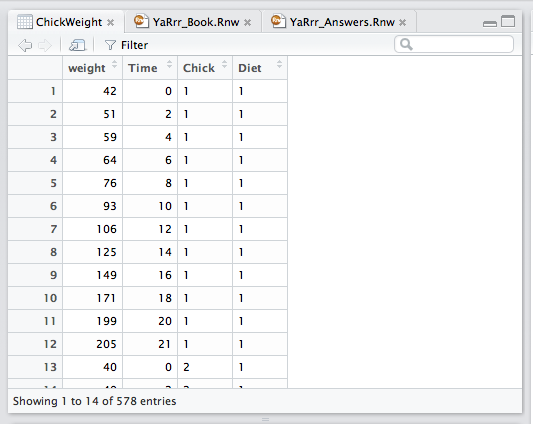
\includegraphics[width=500px]{images/chickweightscreenshot} 

}

\caption{Screenshot of the window from View(ChickWeight). You can use this window to visually sort and filter the data to get an idea of how it looks, but you can't add or remove data and nothing you do will actually change the dataframe.}\label{fig:viewchicks}
\end{figure}

\subsection{\texorpdfstring{\texttt{summary()},
\texttt{str()}}{summary(), str()}}\label{summary-str}

To get summary statistics on all columns in a dataframe, use the
\texttt{summary()} function:

\begin{Shaded}
\begin{Highlighting}[]
\CommentTok{# Print summary statistics of ToothGrowth to the console}
\KeywordTok{summary}\NormalTok{(ToothGrowth)}
\NormalTok{##       len     supp         dose          len.cm        index   }
\NormalTok{##  Min.   : 4   OJ:30   Min.   :0.50   Min.   :0.4   Min.   : 1  }
\NormalTok{##  1st Qu.:13   VC:30   1st Qu.:0.50   1st Qu.:1.3   1st Qu.:16  }
\NormalTok{##  Median :19           Median :1.00   Median :1.9   Median :30  }
\NormalTok{##  Mean   :19           Mean   :1.17   Mean   :1.9   Mean   :30  }
\NormalTok{##  3rd Qu.:25           3rd Qu.:2.00   3rd Qu.:2.5   3rd Qu.:45  }
\NormalTok{##  Max.   :34           Max.   :2.00   Max.   :3.4   Max.   :60}
\end{Highlighting}
\end{Shaded}

To learn about the classes of columns in a dataframe, in addition to
some other summary information, use the \texttt{str()} (structure)
function. This function returns information for more advanced R users,
so don't worry if the output looks confusing.

\begin{Shaded}
\begin{Highlighting}[]
\CommentTok{# Print additional information about ToothGrowth to the console}
\KeywordTok{str}\NormalTok{(ToothGrowth)}
\NormalTok{## 'data.frame':    60 obs. of  5 variables:}
\NormalTok{##  $ len   : num  4.2 11.5 7.3 5.8 6.4 10 11.2 11.2 5.2 7 ...}
\NormalTok{##  $ supp  : Factor w/ 2 levels "OJ","VC": 2 2 2 2 2 2 2 2 2 2 ...}
\NormalTok{##  $ dose  : num  0.5 0.5 0.5 0.5 0.5 0.5 0.5 0.5 0.5 0.5 ...}
\NormalTok{##  $ len.cm: num  0.42 1.15 0.73 0.58 0.64 1 1.12 1.12 0.52 0.7 ...}
\NormalTok{##  $ index : int  1 2 3 4 5 6 7 8 9 10 ...}
\end{Highlighting}
\end{Shaded}

Here, we can see that \texttt{ToothGrowth} is a dataframe with 60
observations (ie., rows) and 3 variables (ie., columns). We can also see
that the column names are \texttt{len}, \texttt{supp}, and \texttt{dose}

\section{Dataframe column names}\label{dataframe-column-names}

One of the nice things about dataframes is that each column will have a
name. You can use these name to access specific columns by name without
having to know which column number it is.

To access the names of a dataframe, use the function \texttt{names()}.
This will return a string vector with the names of the dataframe. Let's
use \texttt{names()} to get the names of the \texttt{ToothGrowth}
dataframe:

\begin{Shaded}
\begin{Highlighting}[]
\CommentTok{# What are the names of columns in the ToothGrowth dataframe?}
\KeywordTok{names}\NormalTok{(ToothGrowth)}
\NormalTok{## [1] "len"    "supp"   "dose"   "len.cm" "index"}
\end{Highlighting}
\end{Shaded}

To access a specific column in a dataframe by name, you use the
\texttt{\$} operator in the form \texttt{df\$name} where \texttt{df} is
the name of the dataframe, and \texttt{name} is the name of the column
you are interested in. This operation will then return the column you
want as a vector.

Let's use the \texttt{\$} operator to get a vector of just the length
column (called \texttt{len}) from the \texttt{ToothGrowth} dataframe:

\begin{Shaded}
\begin{Highlighting}[]
\CommentTok{# Return the len column of ToothGrowth}
\NormalTok{ToothGrowth$len}
\NormalTok{##  [1]  4.2 11.5  7.3  5.8  6.4 10.0 11.2 11.2  5.2  7.0 16.5 16.5 15.2 17.3}
\NormalTok{## [15] 22.5 17.3 13.6 14.5 18.8 15.5 23.6 18.5 33.9 25.5 26.4 32.5 26.7 21.5}
\NormalTok{## [29] 23.3 29.5 15.2 21.5 17.6  9.7 14.5 10.0  8.2  9.4 16.5  9.7 19.7 23.3}
\NormalTok{## [43] 23.6 26.4 20.0 25.2 25.8 21.2 14.5 27.3 25.5 26.4 22.4 24.5 24.8 30.9}
\NormalTok{## [57] 26.4 27.3 29.4 23.0}
\end{Highlighting}
\end{Shaded}

Because the \texttt{\$} operator returns a vector, you can easily
calculate descriptive statistics on columns of a dataframe by applying
your favorite vector function (like \texttt{mean()} or \texttt{table()})
to a column using \texttt{\$}. Let's calculate the mean tooth length
with \texttt{mean()}, and the frequency of each supplement with
\texttt{table()}:

\begin{Shaded}
\begin{Highlighting}[]
\CommentTok{# What is the mean of the len column of ToothGrowth?}
\KeywordTok{mean}\NormalTok{(ToothGrowth$len)}
\NormalTok{## [1] 19}

\CommentTok{# Give me a table of the supp column of ToothGrowth.}
\KeywordTok{table}\NormalTok{(ToothGrowth$supp)}
\NormalTok{## }
\NormalTok{## OJ VC }
\NormalTok{## 30 30}
\end{Highlighting}
\end{Shaded}

If you want to access several columns by name, you can forgo the \$
operator, and put a character vector of column names in brackets:

\begin{Shaded}
\begin{Highlighting}[]
\CommentTok{# Give me the len AND supp columns of ToothGrowth}
\KeywordTok{head}\NormalTok{(ToothGrowth[}\KeywordTok{c}\NormalTok{(}\StringTok{"len"}\NormalTok{, }\StringTok{"supp"}\NormalTok{)])}
\NormalTok{##    len supp}
\NormalTok{## 1  4.2   VC}
\NormalTok{## 2 11.5   VC}
\NormalTok{## 3  7.3   VC}
\NormalTok{## 4  5.8   VC}
\NormalTok{## 5  6.4   VC}
\NormalTok{## 6 10.0   VC}
\end{Highlighting}
\end{Shaded}

\subsection{Adding new columns}\label{adding-new-columns}

You can add new columns to a dataframe using the \texttt{\$} and
assignment \texttt{\textless{}-} operators. To do this, just use the
\texttt{df\$name} notation and assign a new vector of data to it.

For example, let's create a dataframe called \texttt{survey} with two
columns: \texttt{index} and \texttt{age}:

\begin{Shaded}
\begin{Highlighting}[]
\CommentTok{# Create a new dataframe called survey}
\NormalTok{survey <-}\StringTok{ }\KeywordTok{data.frame}\NormalTok{(}\StringTok{"index"} \NormalTok{=}\StringTok{ }\KeywordTok{c}\NormalTok{(}\DecValTok{1}\NormalTok{, }\DecValTok{2}\NormalTok{, }\DecValTok{3}\NormalTok{, }\DecValTok{4}\NormalTok{, }\DecValTok{5}\NormalTok{),}
                     \StringTok{"age"} \NormalTok{=}\StringTok{ }\KeywordTok{c}\NormalTok{(}\DecValTok{24}\NormalTok{, }\DecValTok{25}\NormalTok{, }\DecValTok{42}\NormalTok{, }\DecValTok{56}\NormalTok{, }\DecValTok{22}\NormalTok{))}

\NormalTok{survey}
\NormalTok{##   index age}
\NormalTok{## 1     1  24}
\NormalTok{## 2     2  25}
\NormalTok{## 3     3  42}
\NormalTok{## 4     4  56}
\NormalTok{## 5     5  22}
\end{Highlighting}
\end{Shaded}

Now, let's add a new column called \texttt{sex} with a vector of sex
data:

\begin{Shaded}
\begin{Highlighting}[]
\CommentTok{# Add a new column called sex to survey}
\NormalTok{survey$sex <-}\StringTok{ }\KeywordTok{c}\NormalTok{(}\StringTok{"m"}\NormalTok{, }\StringTok{"m"}\NormalTok{, }\StringTok{"f"}\NormalTok{, }\StringTok{"f"}\NormalTok{, }\StringTok{"m"}\NormalTok{)}
\end{Highlighting}
\end{Shaded}

Here's the result

\begin{Shaded}
\begin{Highlighting}[]
\CommentTok{# survey with new sex column}
\NormalTok{survey}
\NormalTok{##   index age sex}
\NormalTok{## 1     1  24   m}
\NormalTok{## 2     2  25   m}
\NormalTok{## 3     3  42   f}
\NormalTok{## 4     4  56   f}
\NormalTok{## 5     5  22   m}
\end{Highlighting}
\end{Shaded}

As you can see, \texttt{survey} has a new column with the name
\texttt{sex} with the values we specified earlier.

\subsection{Changing column names}\label{changing-column-names}

To change the name of a column in a dataframe, just use a combination of
the \texttt{names()} function, indexing, and reassignment.

\begin{Shaded}
\begin{Highlighting}[]
\CommentTok{# Change name of 1st column of df to "a"}
\KeywordTok{names}\NormalTok{(df)[}\DecValTok{1}\NormalTok{] <-}\StringTok{ "a"}

\CommentTok{# Change name of 2nd column of df to "b"}
\KeywordTok{names}\NormalTok{(df)[}\DecValTok{2}\NormalTok{] <-}\StringTok{ "b"}
\end{Highlighting}
\end{Shaded}

For example, let's change the name of the first column of
\texttt{survey} from \texttt{index} to \texttt{participant.number}

\begin{Shaded}
\begin{Highlighting}[]
\CommentTok{# Change the name of the first column of survey to "participant.number"}
\KeywordTok{names}\NormalTok{(survey)[}\DecValTok{1}\NormalTok{] <-}\StringTok{ "participant.number"}
\NormalTok{survey}
\NormalTok{##   participant.number age sex}
\NormalTok{## 1                  1  24   m}
\NormalTok{## 2                  2  25   m}
\NormalTok{## 3                  3  42   f}
\NormalTok{## 4                  4  56   f}
\NormalTok{## 5                  5  22   m}
\end{Highlighting}
\end{Shaded}

\textbf{Warning!!!}: Change column names with logical indexing to avoid
errors!

Now, there is one major potential problem with my method above -- I had
to manually enter the value of 1. But what if the column I want to
change isn't in the first column (either because I typed it wrong or
because the order of the columns changed)? This could lead to serious
problems later on.

To avoid these issues, it's better to change column names using a
logical vector using the format
\texttt{names(df){[}names(df)\ ==\ "old.name"{]}\ \textless{}-\ "new.name"}.
Here's how to read this: ``Change the names of \texttt{df}, but only
where the original name was \texttt{"old.name"}, to \texttt{"new.name"}.

Let's use logical indexing to change the name of the column
\texttt{survey\$age} to \texttt{survey\$years}:

\begin{Shaded}
\begin{Highlighting}[]
\CommentTok{# Change the column name from age to age.years}
\KeywordTok{names}\NormalTok{(survey)[}\KeywordTok{names}\NormalTok{(survey) ==}\StringTok{ "age"}\NormalTok{] <-}\StringTok{ "years"}
\NormalTok{survey}
\NormalTok{##   participant.number years sex}
\NormalTok{## 1                  1    24   m}
\NormalTok{## 2                  2    25   m}
\NormalTok{## 3                  3    42   f}
\NormalTok{## 4                  4    56   f}
\NormalTok{## 5                  5    22   m}
\end{Highlighting}
\end{Shaded}

\section{Slicing dataframes}\label{slicing-dataframes}

Once you have a dataset stored as a matrix or dataframe in R, you'll
want to start accessing specific parts of the data based on some
criteria. For example, if your dataset contains the result of an
experiment comparing different experimental groups, you'll want to
calculate statistics for each experimental group separately. The process
of selecting specific rows and columns of data based on some criteria is
commonly known as \emph{slicing}.

\begin{figure}

{\centering \includegraphics[width=250px]{images/turnip} 

}

\caption{Slicing and dicing data. The turnip represents your data, and the knife represents indexing with brackets, or subsetting functions like subset(). The red-eyed clown holding the knife is just off camera.}\label{fig:unnamed-chunk-190}
\end{figure}

\subsection{\texorpdfstring{Slicing with
\texttt{{[},\ {]}}}{Slicing with {[}, {]}}}\label{slicing-with}

Just like vectors, you can access specific data in dataframes using
brackets. But now, instead of just using one indexing vector, we use two
indexing vectors: one for the rows and one for the columns. To do this,
use the notation \texttt{data{[}rows,\ columns{]}}, where \texttt{rows}
and \texttt{columns} are vectors of integers.

\begin{Shaded}
\begin{Highlighting}[]
\CommentTok{# Return row 1}
\NormalTok{df[}\DecValTok{1}\NormalTok{, ]}

\CommentTok{# Return column 5}
\NormalTok{df[, }\DecValTok{5}\NormalTok{]}

\CommentTok{# Rows 1:5 and column 2}
\NormalTok{df[}\DecValTok{1}\NormalTok{:}\DecValTok{5}\NormalTok{, }\DecValTok{2}\NormalTok{]}
\end{Highlighting}
\end{Shaded}

\begin{figure}

{\centering \includegraphics[width=300px]{images/guineapig} 

}

\caption{Ah the ToothGrowth dataframe. Yes, one of the dataframes stored in R contains data from an experiment testing the effectiveness of different doses of Vitamin C supplements on the growth of guinea pig teeth. The images I found by Googling ``guinea pig teeth'' were all pretty horrifying, so let's just go with this one.}\label{fig:unnamed-chunk-192}
\end{figure}

\begin{table}

\caption{\label{tab:unnamed-chunk-193}First few rows of the ToothGrowth dataframe.}
\centering
\begin{tabular}[t]{r|l|r|r|r}
\hline
len & supp & dose & len.cm & index\\
\hline
4.2 & VC & 0.5 & 0.42 & 1\\
\hline
11.5 & VC & 0.5 & 1.15 & 2\\
\hline
7.3 & VC & 0.5 & 0.73 & 3\\
\hline
5.8 & VC & 0.5 & 0.58 & 4\\
\hline
6.4 & VC & 0.5 & 0.64 & 5\\
\hline
10.0 & VC & 0.5 & 1.00 & 6\\
\hline
\end{tabular}
\end{table}

Let's try indexing the \texttt{ToothGrowth} dataframe. Again, the
\texttt{ToothGrowth} dataframe represents the results of a study testing
the effectiveness of different types of supplements on the length of
guinea pig's teeth. First, let's look at the entries in rows 1 through
5, and column 1:

\begin{Shaded}
\begin{Highlighting}[]
\CommentTok{# Give me the rows 1-6 and column 1 of ToothGrowth}
\NormalTok{ToothGrowth[}\DecValTok{1}\NormalTok{:}\DecValTok{6}\NormalTok{, }\DecValTok{1}\NormalTok{]}
\NormalTok{## [1]  4.2 11.5  7.3  5.8  6.4 10.0}
\end{Highlighting}
\end{Shaded}

Because the first column is \texttt{len}, the primary dependent measure,
this means that the tooth lengths in the first 5 observations are 4.2,
11.5, 7.3, 5.8, 6.4, 10.

Of course, you can index matrices and dataframes with longer vectors to
get more data. Now, let's look at the first 3 rows of columns 1 and 3:

\begin{Shaded}
\begin{Highlighting}[]
\CommentTok{# Give me rows 1-3 and columns 1 and 3 of ToothGrowth}
\NormalTok{ToothGrowth[}\DecValTok{1}\NormalTok{:}\DecValTok{3}\NormalTok{, }\KeywordTok{c}\NormalTok{(}\DecValTok{1}\NormalTok{,}\DecValTok{3}\NormalTok{)]}
\NormalTok{##    len dose}
\NormalTok{## 1  4.2  0.5}
\NormalTok{## 2 11.5  0.5}
\NormalTok{## 3  7.3  0.5}
\end{Highlighting}
\end{Shaded}

If you want to look at an entire row or an entire column of a matrix or
dataframe, you can leave the corresponding index blank. For example, to
see the entire 1st row of the \texttt{ToothGrowth} dataframe, we can set
the row index to 1, and leave the column index blank:

\begin{Shaded}
\begin{Highlighting}[]
\CommentTok{# Give me the 1st row (and all columns) of ToothGrowth}
\NormalTok{ToothGrowth[}\DecValTok{1}\NormalTok{, ]}
\NormalTok{##   len supp dose len.cm index}
\NormalTok{## 1 4.2   VC  0.5   0.42     1}
\end{Highlighting}
\end{Shaded}

Similarly, to get the entire 2nd column, set the column index to 2 and
leave the row index blank:

\begin{Shaded}
\begin{Highlighting}[]
\CommentTok{# Give me the 2nd column (and all rows) of ToothGrowth}
\NormalTok{ToothGrowth[, }\DecValTok{2}\NormalTok{]}
\NormalTok{##  [1] VC VC VC VC VC VC VC VC VC VC VC VC VC VC VC VC VC VC VC VC VC VC VC}
\NormalTok{## [24] VC VC VC VC VC VC VC OJ OJ OJ OJ OJ OJ OJ OJ OJ OJ OJ OJ OJ OJ OJ OJ}
\NormalTok{## [47] OJ OJ OJ OJ OJ OJ OJ OJ OJ OJ OJ OJ OJ OJ}
\NormalTok{## Levels: OJ VC}
\end{Highlighting}
\end{Shaded}

Many, if not all, of the analyses you will be doing will be on subsets
of data, rather than entire datasets. For example, if you have data from
an experiment, you may wish to calculate the mean of participants in one
group separately from another. To do this, we'll use \emph{subsetting}
-- selecting subsets of data based on some criteria. To do this, we can
use one of two methods: indexing with logical vectors, or the
\texttt{subset()} function. We'll start with logical indexing first.

\subsection{Slicing with logical
vectors}\label{slicing-with-logical-vectors}

Indexing dataframes with logical vectors is almost identical to indexing
single vectors. First, we create a logical vector containing only TRUE
and FALSE values. Next, we index a dataframe (typically the rows) using
the logical vector to return \emph{only} values for which the logical
vector is TRUE.

For example, to create a new dataframe called \texttt{ToothGrowth.VC}
containing only data from the guinea pigs who were given the VC
supplement, we'd run the following code:

\begin{Shaded}
\begin{Highlighting}[]
\CommentTok{# Create a new df with only the rows of ToothGrowth}
\CommentTok{#  where supp equals VC}
\NormalTok{ToothGrowth.VC <-}\StringTok{ }\NormalTok{ToothGrowth[ToothGrowth$supp ==}\StringTok{ "VC"}\NormalTok{, ]}
\end{Highlighting}
\end{Shaded}

Of course, just like we did with vectors, we can make logical vectors
based on multiple criteria -- and then index a dataframe based on those
criteria. For example, let's create a dataframe called
\texttt{ToothGrowth.OJ.a} that contains data from the guinea pigs who
were given an OJ supplement with a dose less than 1.0:

\begin{Shaded}
\begin{Highlighting}[]
\CommentTok{# Create a new df with only the rows of ToothGrowth}
\CommentTok{#  where supp equals OJ and dose < 1}

\NormalTok{ToothGrowth.VC.a <-}\StringTok{ }\NormalTok{ToothGrowth[ToothGrowth$supp ==}\StringTok{ "OJ"} \NormalTok{&}
\StringTok{                                }\NormalTok{ToothGrowth$dose <}\StringTok{ }\DecValTok{1}\NormalTok{, ]}
\end{Highlighting}
\end{Shaded}

Indexing with brackets is the standard way to slice and dice dataframes.
However, the code can get a bit messy. A more elegant method is to use
the \texttt{subset()} function.

\subsection{\texorpdfstring{Slicing with
\texttt{subset()}}{Slicing with subset()}}\label{slicing-with-subset}

\begin{figure}

{\centering \includegraphics[width=400px]{images/saber} 

}

\caption{The subset() function is like a lightsaber. An elegant function from a more civilized age.}\label{fig:unnamed-chunk-200}
\end{figure}

The \texttt{subset()} function is one of the most useful data management
functions in R. It allows you to slice and dice datasets just like you
would with brackets, but the code is much easier to write: Table
\ref{tab:subsetfunction} shows the main arguments to the
\texttt{subset()} function:

\begin{longtable}[]{@{}ll@{}}
\caption{\label{tab:subsetfunction} Main arguments for the \texttt{subset()}
function.}\tabularnewline
\toprule
Argument & Description\tabularnewline
\midrule
\endfirsthead
\toprule
Argument & Description\tabularnewline
\midrule
\endhead
\texttt{x} & A dataframe you want to subset\tabularnewline
\texttt{subset} & A logical vector indicating the rows to
keep\tabularnewline
\texttt{select} & The columns you want to keep\tabularnewline
\bottomrule
\end{longtable}

Let's use the \texttt{subset()} function to create a new, subsetted
dataset from the \texttt{ToothGrowth} dataframe containing data from
guinea pigs who had a tooth length less than 20cm
(\texttt{len\ \textless{}\ 20}), given the OJ supplement
(\texttt{supp\ ==\ "OJ"}), and with a dose greater than or equal to 1
(\texttt{dose\ \textgreater{}=\ 1}):

\begin{Shaded}
\begin{Highlighting}[]
\CommentTok{# Get rows of ToothGrowth where len < 20 AND supp == "OJ" AND dose >= 1}

\KeywordTok{subset}\NormalTok{(}\DataTypeTok{x =} \NormalTok{ToothGrowth,}
      \DataTypeTok{subset =} \NormalTok{len <}\StringTok{ }\DecValTok{20} \NormalTok{&}
\StringTok{               }\NormalTok{supp ==}\StringTok{ "OJ"} \NormalTok{&}
\StringTok{               }\NormalTok{dose >=}\StringTok{ }\DecValTok{1}\NormalTok{)}
\NormalTok{##    len supp dose len.cm index}
\NormalTok{## 41  20   OJ    1    2.0    41}
\NormalTok{## 49  14   OJ    1    1.4    49}
\end{Highlighting}
\end{Shaded}

As you can see, there were only two cases that satisfied all 3 of our
selection criteria.

In the example above, I didn't specify an input to the \texttt{select}
argument because I wanted all columns. However, if you just want certain
columns, you can just name the columns you want in the \texttt{select}
argument:

\begin{Shaded}
\begin{Highlighting}[]
\CommentTok{# Get rows of ToothGrowth where len > 30 AND supp == "VC", but only return the len and index columns}

\KeywordTok{subset}\NormalTok{(}\DataTypeTok{x =} \NormalTok{ToothGrowth,}
      \DataTypeTok{subset =} \NormalTok{len >}\StringTok{ }\DecValTok{30} \NormalTok{&}
\StringTok{               }\NormalTok{supp ==}\StringTok{ "VC"}\NormalTok{,}
      \DataTypeTok{select =} \KeywordTok{c}\NormalTok{(len, index))}
\NormalTok{##    len index}
\NormalTok{## 23  34    23}
\NormalTok{## 26  32    26}
\end{Highlighting}
\end{Shaded}

\section{Combining slicing with
functions}\label{combining-slicing-with-functions}

Now that you know how to slice and dice dataframes using indexing and
\texttt{subset()}, you can easily combine slicing and dicing with
statistical functions to calculate summary statistics on groups of data.
For example, the following code will calculate the mean tooth length of
guinea pigs with the OJ supplement using the \texttt{subset()} function:

\begin{Shaded}
\begin{Highlighting}[]
\CommentTok{# What is the mean tooth length of Guinea pigs given OJ?}

\CommentTok{# Step 1: Create a subsettted dataframe called oj}

\NormalTok{oj <-}\StringTok{ }\KeywordTok{subset}\NormalTok{(}\DataTypeTok{x =} \NormalTok{ToothGrowth,}
             \DataTypeTok{subset =} \NormalTok{supp ==}\StringTok{ "OJ"}\NormalTok{)}

\CommentTok{# Step 2: Calculate the mean of the len column from}
\CommentTok{#  the new subsetted dataset}

\KeywordTok{mean}\NormalTok{(oj$len)}
\NormalTok{## [1] 21}
\end{Highlighting}
\end{Shaded}

We can also get the same solution using logical indexing:

\begin{Shaded}
\begin{Highlighting}[]
\CommentTok{# Step 1: Create a subsettted dataframe called oj}
\NormalTok{oj <-}\StringTok{ }\NormalTok{ToothGrowth[ToothGrowth$supp ==}\StringTok{ "OJ"}\NormalTok{,]}

\CommentTok{# Step 2: Calculate the mean of the len column from}
\CommentTok{#  the new subsetted dataset}
\KeywordTok{mean}\NormalTok{(oj$len)}
\NormalTok{## [1] 21}
\end{Highlighting}
\end{Shaded}

Or heck, we can do it all in one line by only referring to column
vectors:

\begin{Shaded}
\begin{Highlighting}[]
\KeywordTok{mean}\NormalTok{(ToothGrowth$len[ToothGrowth$supp ==}\StringTok{ "OJ"}\NormalTok{])}
\NormalTok{## [1] 21}
\end{Highlighting}
\end{Shaded}

As you can see, R allows for many methods to accomplish the same task.
The choice is up to you.

\subsection{\texorpdfstring{\texttt{with()}}{with()}}\label{with}

The \texttt{with()} function helps to save you some typing when you are
using multiple columns from a dataframe. Specifically, it allows you to
specify a dataframe (or any other object in R) once at the beginning of
a line -- then, for every object you refer to in the code in that line,
R will assume you're referring to that object in an expression.

For example, let's create a dataframe called \texttt{health} with some
health information:

\begin{Shaded}
\begin{Highlighting}[]
\NormalTok{health <-}\StringTok{ }\KeywordTok{data.frame}\NormalTok{(}\StringTok{"age"} \NormalTok{=}\StringTok{ }\KeywordTok{c}\NormalTok{(}\DecValTok{32}\NormalTok{, }\DecValTok{24}\NormalTok{, }\DecValTok{43}\NormalTok{, }\DecValTok{19}\NormalTok{, }\DecValTok{43}\NormalTok{),}
                     \StringTok{"height"} \NormalTok{=}\StringTok{ }\KeywordTok{c}\NormalTok{(}\FloatTok{1.75}\NormalTok{, }\FloatTok{1.65}\NormalTok{, }\FloatTok{1.50}\NormalTok{, }\FloatTok{1.92}\NormalTok{, }\FloatTok{1.80}\NormalTok{),}
                     \StringTok{"weight"} \NormalTok{=}\StringTok{ }\KeywordTok{c}\NormalTok{(}\DecValTok{70}\NormalTok{, }\DecValTok{65}\NormalTok{, }\DecValTok{62}\NormalTok{, }\DecValTok{79}\NormalTok{, }\DecValTok{85}\NormalTok{))}

\NormalTok{health}
\NormalTok{##   age height weight}
\NormalTok{## 1  32    1.8     70}
\NormalTok{## 2  24    1.6     65}
\NormalTok{## 3  43    1.5     62}
\NormalTok{## 4  19    1.9     79}
\NormalTok{## 5  43    1.8     85}
\end{Highlighting}
\end{Shaded}

Now let's say we want to add a new column called \texttt{bmi} which
represents a person's body mass index. The formula for bmi is
\(bmi = \frac{height}{weight^{2}} \times 703\). If we wanted to
calculate the bmi of each person, we'd need to write
\texttt{health\$height\ /\ health\$weight\ \^{}\ 2}:

\begin{Shaded}
\begin{Highlighting}[]
\CommentTok{# Calculate bmi}
\NormalTok{health$weight /}\StringTok{ }\NormalTok{health$height ^}\StringTok{ }\DecValTok{2}
\NormalTok{## [1] 23 24 28 21 26}
\end{Highlighting}
\end{Shaded}

As you can see, we have to retype the name of the dataframe for each
column. However, using the \texttt{with()} function, we can make it a
bit easier by saying the name of the dataframe once.

\begin{Shaded}
\begin{Highlighting}[]
\CommentTok{# Save typing by using with()}
\KeywordTok{with}\NormalTok{(health, weight /}\StringTok{ }\NormalTok{height ^}\StringTok{ }\DecValTok{2}\NormalTok{)}
\NormalTok{## [1] 23 24 28 21 26}
\end{Highlighting}
\end{Shaded}

As you can see, the results are identical. In this case, we didn't save
so much typing. But if you are doing many calculations, then
\texttt{with()} can save you a lot of typing. For example, contrast
these two lines of code that perform identical calculations:

\begin{Shaded}
\begin{Highlighting}[]
\CommentTok{# Long code}
\NormalTok{health$weight +}\StringTok{ }\NormalTok{health$height /}\StringTok{ }\NormalTok{health$age +}\StringTok{ }\DecValTok{2} \NormalTok{*}\StringTok{ }\NormalTok{health$height}
\NormalTok{## [1] 74 68 65 83 89}

\CommentTok{# Short code that does the same thing}
\KeywordTok{with}\NormalTok{(health, weight +}\StringTok{ }\NormalTok{height /}\StringTok{ }\NormalTok{age +}\StringTok{ }\DecValTok{2} \NormalTok{*}\StringTok{ }\NormalTok{height)}
\NormalTok{## [1] 74 68 65 83 89}
\end{Highlighting}
\end{Shaded}

\section{Test your R might! Pirates and
superheroes}\label{test-your-r-might-pirates-and-superheroes}

\begin{figure}

{\centering \includegraphics[width=300px]{images/maggot} 

}

\caption{This is a lesser-known superhero named Maggott who could 'transform his body to get superhuman strength and endurance, but to do so he needed to release two huge parasitic worms from his stomach cavity and have them eat things' (http://heavy.com/comedy/2010/04/the-20-worst-superheroes/). Yeah...I'm shocked this guy wasn't a hit.}\label{fig:unnamed-chunk-210}
\end{figure}

The following table shows the results of a survey of 10 pirates. In
addition to some basic demographic information, the survey asked each
pirate ``What is your favorite superhero?''" and ``How many tattoos do
you have?''"

\begin{tabular}{l|l|r|l|r}
\hline
Name & Sex & Age & Superhero & Tattoos\\
\hline
Astrid & F & 30 & Batman & 11\\
\hline
Lea & F & 25 & Superman & 15\\
\hline
Sarina & F & 25 & Batman & 12\\
\hline
Remon & M & 29 & Spiderman & 5\\
\hline
Letizia & F & 22 & Batman & 65\\
\hline
Babice & F & 22 & Antman & 3\\
\hline
Jonas & M & 35 & Batman & 9\\
\hline
Wendy & F & 19 & Superman & 13\\
\hline
Niveditha & F & 32 & Maggott & 900\\
\hline
Gioia & F & 21 & Superman & 0\\
\hline
\end{tabular}

\begin{enumerate}
\def\labelenumi{\arabic{enumi}.}
\item
  Combine the data into a single dataframe. Complete all the following
  exercises from the dataframe!
\item
  What is the median age of the 10 pirates?
\item
  What was the mean age of female and male pirates separately?
\item
  What was the most number of tattoos owned by a male pirate?
\item
  What percent of pirates under the age of 32 were female?
\item
  What percent of female pirates are under the age of 32?
\item
  Add a new column to the dataframe called \texttt{tattoos.per.year}
  which shows how many tattoos each pirate has for each year in their
  life.
\item
  Which pirate had the most number of tattoos per year?
\item
  What are the names of the female pirates whose favorite superhero is
  Superman?
\item
  What was the median number of tattoos of pirates over the age of 20
  whose favorite superhero is Spiderman?
\end{enumerate}

\chapter{Test your R might!
Solutions}\label{test-your-r-might-solutions}

\section{Chapter 4: The Basics}\label{chapter-4-the-basics}

\begin{enumerate}
\def\labelenumi{\arabic{enumi}.}
\setcounter{enumi}{1}
\tightlist
\item
  Which (if any) of the following objects names is/are invalid?
\end{enumerate}

\begin{Shaded}
\begin{Highlighting}[]
\NormalTok{thisone <-}\StringTok{ }\DecValTok{1}
\NormalTok{THISONE <-}\StringTok{ }\DecValTok{2}
\NormalTok{this.one <-}\StringTok{ }\DecValTok{3}
\NormalTok{This}\FloatTok{.1} \NormalTok{<-}\StringTok{ }\DecValTok{4}
\NormalTok{ThIS.....ON...E <-}\StringTok{ }\DecValTok{5}
\NormalTok{This!One!}\StringTok{ }\ErrorTok{<}\NormalTok{-}\StringTok{ }\DecValTok{6}           \CommentTok{# only this one!}
\NormalTok{lkjasdfkjsdf <-}\StringTok{ }\DecValTok{7}
\end{Highlighting}
\end{Shaded}

\begin{enumerate}
\def\labelenumi{\arabic{enumi}.}
\setcounter{enumi}{2}
\tightlist
\item
  2015 was a good year for pirate booty - your ship collected 100,000
  gold coins. Create an object called \texttt{gold.in.2015} and assign
  the correct value to it.
\end{enumerate}

\begin{Shaded}
\begin{Highlighting}[]
\NormalTok{gold.in}\FloatTok{.2015} \NormalTok{<-}\StringTok{ }\DecValTok{100800}
\end{Highlighting}
\end{Shaded}

\begin{enumerate}
\def\labelenumi{\arabic{enumi}.}
\setcounter{enumi}{3}
\tightlist
\item
  Oops, during the last inspection we discovered that one of your
  pirates Skippy McGee hid 800 gold coins in his underwear. Go ahead and
  add those gold coins to the object \texttt{gold.in.2015}. Next, create
  an object called \texttt{plank.list} with the name of the pirate
  thief.
\end{enumerate}

\begin{Shaded}
\begin{Highlighting}[]
\NormalTok{gold.in}\FloatTok{.2015} \NormalTok{<-}\StringTok{ }\NormalTok{gold.in}\FloatTok{.2015} \NormalTok{+}\StringTok{ }\DecValTok{800}
\NormalTok{plank.list <-}\StringTok{ "Skippy McGee"}
\end{Highlighting}
\end{Shaded}

\begin{enumerate}
\def\labelenumi{\arabic{enumi}.}
\setcounter{enumi}{4}
\tightlist
\item
  Look at the code below. What will R return after the third line? Make
  a prediction, then test the code yourself.
\end{enumerate}

\begin{Shaded}
\begin{Highlighting}[]
\NormalTok{a <-}\StringTok{ }\DecValTok{10}
\NormalTok{a +}\StringTok{ }\DecValTok{10}
\NormalTok{a       }\CommentTok{# It will return 10 because we never re-assigned a!}
\end{Highlighting}
\end{Shaded}

\section{Chapter 5: Scalers and
vectors}\label{chapter-5-scalers-and-vectors}

\begin{enumerate}
\def\labelenumi{\arabic{enumi}.}
\tightlist
\item
  Create the vector {[}1, 2, 3, 4, 5, 6, 7, 8, 9, 10{]} in three ways:
  once using \texttt{c()}, once using \texttt{a:b}, and once using
  \texttt{seq()}.
\end{enumerate}

\begin{Shaded}
\begin{Highlighting}[]
\KeywordTok{c}\NormalTok{(}\DecValTok{1}\NormalTok{, }\DecValTok{2}\NormalTok{, }\DecValTok{3}\NormalTok{, }\DecValTok{4}\NormalTok{, }\DecValTok{5}\NormalTok{, }\DecValTok{6}\NormalTok{, }\DecValTok{7}\NormalTok{, }\DecValTok{8}\NormalTok{, }\DecValTok{9}\NormalTok{, }\DecValTok{10}\NormalTok{)}
\NormalTok{##  [1]  1  2  3  4  5  6  7  8  9 10}

\DecValTok{1}\NormalTok{:}\DecValTok{10}
\NormalTok{##  [1]  1  2  3  4  5  6  7  8  9 10}

\KeywordTok{seq}\NormalTok{(}\DataTypeTok{from =} \DecValTok{1}\NormalTok{, }\DataTypeTok{to =} \DecValTok{10}\NormalTok{, }\DataTypeTok{by =} \DecValTok{1}\NormalTok{)}
\NormalTok{##  [1]  1  2  3  4  5  6  7  8  9 10}
\end{Highlighting}
\end{Shaded}

\begin{enumerate}
\def\labelenumi{\arabic{enumi}.}
\setcounter{enumi}{1}
\tightlist
\item
  Create the vector {[}2.1, 4.1, 6.1, 8.1{]} in two ways, once using
  \texttt{c()} and once using \texttt{seq()}
\end{enumerate}

\begin{Shaded}
\begin{Highlighting}[]

\KeywordTok{c}\NormalTok{(}\FloatTok{2.1}\NormalTok{, }\FloatTok{6.1}\NormalTok{, }\FloatTok{6.1}\NormalTok{, }\FloatTok{8.1}\NormalTok{)}
\NormalTok{## [1] 2.1 6.1 6.1 8.1}

\KeywordTok{seq}\NormalTok{(}\DataTypeTok{from =} \FloatTok{2.1}\NormalTok{, }\DataTypeTok{to =} \FloatTok{8.1}\NormalTok{, }\DataTypeTok{by =} \DecValTok{2}\NormalTok{)}
\NormalTok{## [1] 2.1 4.1 6.1 8.1}
\end{Highlighting}
\end{Shaded}

\begin{enumerate}
\def\labelenumi{\arabic{enumi}.}
\setcounter{enumi}{2}
\tightlist
\item
  Create the vector {[}0, 5, 10, 15{]} in 3 ways: using \texttt{c()},
  \texttt{seq()} with a \texttt{by} argument, and \texttt{seq()} with a
  \texttt{length.out} argument.
\end{enumerate}

\begin{Shaded}
\begin{Highlighting}[]
\KeywordTok{c}\NormalTok{(}\DecValTok{0}\NormalTok{, }\DecValTok{5}\NormalTok{, }\DecValTok{10}\NormalTok{, }\DecValTok{15}\NormalTok{)}
\NormalTok{## [1]  0  5 10 15}

\KeywordTok{seq}\NormalTok{(}\DataTypeTok{from =} \DecValTok{0}\NormalTok{, }\DataTypeTok{to =} \DecValTok{15}\NormalTok{, }\DataTypeTok{by =} \DecValTok{5}\NormalTok{)}
\NormalTok{## [1]  0  5 10 15}

\KeywordTok{seq}\NormalTok{(}\DataTypeTok{from =} \DecValTok{0}\NormalTok{, }\DataTypeTok{to =} \DecValTok{15}\NormalTok{, }\DataTypeTok{length.out =} \DecValTok{4}\NormalTok{)}
\NormalTok{## [1]  0  5 10 15}
\end{Highlighting}
\end{Shaded}

\begin{enumerate}
\def\labelenumi{\arabic{enumi}.}
\setcounter{enumi}{3}
\tightlist
\item
  Create the vector {[}101, 102, 103, 200, 205, 210, 1000, 1100, 1200{]}
  using a combination of the \texttt{c()} and \texttt{seq()} functions
\end{enumerate}

\begin{Shaded}
\begin{Highlighting}[]
\KeywordTok{c}\NormalTok{(}\KeywordTok{seq}\NormalTok{(}\DataTypeTok{from =} \DecValTok{101}\NormalTok{, }\DataTypeTok{to =} \DecValTok{103}\NormalTok{, }\DataTypeTok{by =} \DecValTok{3}\NormalTok{), }
  \KeywordTok{seq}\NormalTok{(}\DataTypeTok{from =} \DecValTok{200}\NormalTok{, }\DataTypeTok{to =} \DecValTok{210}\NormalTok{, }\DataTypeTok{by =} \DecValTok{5}\NormalTok{), }
  \KeywordTok{seq}\NormalTok{(}\DataTypeTok{from =} \DecValTok{1000}\NormalTok{, }\DataTypeTok{to =} \DecValTok{1200}\NormalTok{, }\DataTypeTok{by =} \DecValTok{100}\NormalTok{))}
\NormalTok{## [1]  101  200  205  210 1000 1100 1200}
\end{Highlighting}
\end{Shaded}

\begin{enumerate}
\def\labelenumi{\arabic{enumi}.}
\setcounter{enumi}{4}
\tightlist
\item
  A new batch of 100 pirates are boarding your ship and need new swords.
  You have 10 scimitars, 40 broadswords, and 50 cutlasses that you need
  to distribute evenly to the 100 pirates as they board. Create a vector
  of length 100 where there is 1 scimitar, 4 broadswords, and 5
  cutlasses in each group of 10. That is, in the first 10 elements there
  should be exactly 1 scimitar, 4 broadswords and 5 cutlasses. The next
  10 elements should also have the same number of each sword (and so
  on).
\end{enumerate}

\begin{Shaded}
\begin{Highlighting}[]
\NormalTok{swords <-}\StringTok{ }\KeywordTok{rep}\NormalTok{(}\KeywordTok{c}\NormalTok{(}\StringTok{"scimitar"}\NormalTok{, }\KeywordTok{rep}\NormalTok{(}\StringTok{"broadswoard"}\NormalTok{, }\DecValTok{4}\NormalTok{), }\KeywordTok{rep}\NormalTok{(}\StringTok{"cutlass"}\NormalTok{, }\DecValTok{5}\NormalTok{)), }\DataTypeTok{times =} \DecValTok{100}\NormalTok{)}
\KeywordTok{head}\NormalTok{(swords)}
\NormalTok{## [1] "scimitar"    "broadswoard" "broadswoard" "broadswoard" "broadswoard"}
\NormalTok{## [6] "cutlass"}
\end{Highlighting}
\end{Shaded}

\begin{enumerate}
\def\labelenumi{\arabic{enumi}.}
\setcounter{enumi}{5}
\tightlist
\item
  Create a vector that repeats the integers from 1 to 5, 10 times. That
  is {[}1, 2, 3, 4, 5, 1, 2, 3, 4, 5, \ldots{}{]}. The length of the
  vector should be 50!
\end{enumerate}

\begin{Shaded}
\begin{Highlighting}[]
\KeywordTok{rep}\NormalTok{(}\DecValTok{1}\NormalTok{:}\DecValTok{5}\NormalTok{, }\DataTypeTok{times =} \DecValTok{10}\NormalTok{)}
\NormalTok{##  [1] 1 2 3 4 5 1 2 3 4 5 1 2 3 4 5 1 2 3 4 5 1 2 3 4 5 1 2 3 4 5 1 2 3 4 5}
\NormalTok{## [36] 1 2 3 4 5 1 2 3 4 5 1 2 3 4 5}
\end{Highlighting}
\end{Shaded}

\begin{enumerate}
\def\labelenumi{\arabic{enumi}.}
\setcounter{enumi}{6}
\tightlist
\item
  Now, create the same vector as before, but this time repeat 1, 10
  times, then 2, 10 times, etc., That is {[}1, 1, 1, \ldots{}, 2, 2, 2,
  \ldots{}, \ldots{} 5, 5, 5{]}. The length of the vector should also be
  50
\end{enumerate}

\begin{Shaded}
\begin{Highlighting}[]
\KeywordTok{rep}\NormalTok{(}\DecValTok{1}\NormalTok{:}\DecValTok{5}\NormalTok{, }\DataTypeTok{each =} \DecValTok{10}\NormalTok{)}
\NormalTok{##  [1] 1 1 1 1 1 1 1 1 1 1 2 2 2 2 2 2 2 2 2 2 3 3 3 3 3 3 3 3 3 3 4 4 4 4 4}
\NormalTok{## [36] 4 4 4 4 4 5 5 5 5 5 5 5 5 5 5}
\end{Highlighting}
\end{Shaded}

\begin{enumerate}
\def\labelenumi{\arabic{enumi}.}
\setcounter{enumi}{7}
\tightlist
\item
  Create a vector containing 50 samples from a Normal distribution with
  a population mean of 20 and standard deviation of 2.
\end{enumerate}

\begin{Shaded}
\begin{Highlighting}[]
\KeywordTok{rnorm}\NormalTok{(}\DataTypeTok{n =} \DecValTok{50}\NormalTok{, }\DataTypeTok{mean =} \DecValTok{20}\NormalTok{, }\DataTypeTok{sd =} \DecValTok{2}\NormalTok{)}
\NormalTok{##  [1] 22 22 19 19 19 20 19 15 19 19 18 20 21 21 21 22 20 21 20 20 21 17 18}
\NormalTok{## [24] 22 20 20 24 22 18 22 23 22 20 19 21 19 18 22 22 24 19 19 15 23 20 22}
\NormalTok{## [47] 21 20 22 17}
\end{Highlighting}
\end{Shaded}

\begin{enumerate}
\def\labelenumi{\arabic{enumi}.}
\setcounter{enumi}{8}
\tightlist
\item
  Create a vector containing 25 samples from a Uniform distribution with
  a lower bound of -100 and an upper bound of -50.
\end{enumerate}

\begin{Shaded}
\begin{Highlighting}[]
\KeywordTok{runif}\NormalTok{(}\DataTypeTok{n =} \DecValTok{25}\NormalTok{, }\DataTypeTok{min =} \NormalTok{-}\DecValTok{100}\NormalTok{, }\DataTypeTok{max =} \NormalTok{-}\DecValTok{50}\NormalTok{)}
\NormalTok{##  [1] -61 -88 -69 -75 -88 -94 -82 -93 -56 -50 -94 -60 -62 -80 -65 -78 -90}
\NormalTok{## [18] -57 -57 -73 -62 -82 -56 -86 -99}
\end{Highlighting}
\end{Shaded}

\section{Chapter 6: Vector Functions}\label{chapter-6-vector-functions}

\begin{enumerate}
\def\labelenumi{\arabic{enumi}.}
\tightlist
\item
  Create a vector that shows the square root of the integers from 1 to
  10.
\end{enumerate}

\begin{Shaded}
\begin{Highlighting}[]
\NormalTok{(}\DecValTok{1}\NormalTok{:}\DecValTok{10}\NormalTok{) ^}\StringTok{ }\NormalTok{.}\DecValTok{5}
\NormalTok{##  [1] 1.0 1.4 1.7 2.0 2.2 2.4 2.6 2.8 3.0 3.2}

\CommentTok{#or}

\KeywordTok{sqrt}\NormalTok{(}\DecValTok{1}\NormalTok{:}\DecValTok{10}\NormalTok{)}
\NormalTok{##  [1] 1.0 1.4 1.7 2.0 2.2 2.4 2.6 2.8 3.0 3.2}
\end{Highlighting}
\end{Shaded}

\begin{enumerate}
\def\labelenumi{\arabic{enumi}.}
\setcounter{enumi}{1}
\tightlist
\item
  Renata thinks that she finds more treasure when she's had a mug of
  grogg than when she doesn't. To test this, she recorded how much
  treasure she found over 7 days without drinking any grogg (ie.,
  sober), and then did the same over 7 days while drinking grogg (ie.,
  drunk). Here are her results:
\end{enumerate}

\begin{table}

\caption{\label{tab:unnamed-chunk-227}Renata's treasure haul when she was sober and when she was drunk}
\centering
\begin{tabular}[t]{l|r|r}
\hline
day & sober & drunk\\
\hline
Monday & 2 & 0\\
\hline
Tuesday & 0 & 0\\
\hline
Wednesday & 3 & 1\\
\hline
Thursday & 1 & 0\\
\hline
Friday & 0 & 1\\
\hline
Saturday & 3 & 2\\
\hline
Sunday & 5 & 2\\
\hline
\end{tabular}
\end{table}

How much treasure did Renata find on average whe she was sober? What
about when she was drunk?

\begin{Shaded}
\begin{Highlighting}[]
\NormalTok{sober <-}\StringTok{ }\KeywordTok{c}\NormalTok{(}\DecValTok{2}\NormalTok{, }\DecValTok{0}\NormalTok{, }\DecValTok{3}\NormalTok{, }\DecValTok{1}\NormalTok{, }\DecValTok{0}\NormalTok{, }\DecValTok{3}\NormalTok{, }\DecValTok{5}\NormalTok{)}
\NormalTok{drunk <-}\StringTok{ }\KeywordTok{c}\NormalTok{(}\DecValTok{0}\NormalTok{, }\DecValTok{0}\NormalTok{, }\DecValTok{1}\NormalTok{, }\DecValTok{0}\NormalTok{, }\DecValTok{1}\NormalTok{, }\DecValTok{2}\NormalTok{, }\DecValTok{2}\NormalTok{)}

\KeywordTok{mean}\NormalTok{(sober)}
\NormalTok{## [1] 2}
\KeywordTok{mean}\NormalTok{(drunk)}
\NormalTok{## [1] 0.86}
\end{Highlighting}
\end{Shaded}

\begin{enumerate}
\def\labelenumi{\arabic{enumi}.}
\setcounter{enumi}{2}
\tightlist
\item
  Using Renata's data again, create a new vector called
  \texttt{difference} that shows how much more treasure Renata found
  when she was drunk and when she was not. What was the mean, median,
  and standard deviation of the difference?
\end{enumerate}

\begin{Shaded}
\begin{Highlighting}[]
\NormalTok{difference <-}\StringTok{ }\NormalTok{sober -}\StringTok{ }\NormalTok{drunk}

\KeywordTok{mean}\NormalTok{(difference)}
\NormalTok{## [1] 1.1}
\KeywordTok{median}\NormalTok{(difference)}
\NormalTok{## [1] 1}
\KeywordTok{sd}\NormalTok{(difference)}
\NormalTok{## [1] 1.3}
\end{Highlighting}
\end{Shaded}

\begin{enumerate}
\def\labelenumi{\arabic{enumi}.}
\setcounter{enumi}{3}
\tightlist
\item
  There's an old parable that goes something like this. A man does some
  work for a king and needs to be paid. Because the man loves rice (who
  doesn't?!), the man offers the king two different ways that he can be
  paid. \emph{You can either pay me 100 kilograms of rice, or, you can
  pay me as follows: get a chessboard and put one grain of rice in the
  top left square. Then put 2 grains of rice on the next square,
  followed by 4 grains on the next, 8 grains on the next\ldots{}and so
  on, where the amount of rice doubles on each square, until you get to
  the last square. When you are finished, give me all the grains of rice
  that would (in theory), fit on the chessboard.} The king, sensing that
  the man was an idiot for making such a stupid offer, immediately
  accepts the second option. He summons a chessboard, and begins
  counting out grains of rice one by one\ldots{} Assuming that there are
  64 squares on a chessboard, calculate how many grains of rice the main
  will receive. If one grain of rice weights 1/64000 kilograms, how many
  kilograms of rice did he get? \emph{Hint: If you have trouble coming
  up with the answer, imagine how many grains are on the first, second,
  third and fourth squares, then try to create the vector that shows the
  number of grains on each square. Once you come up with that vector,
  you can easily calculate the final answer with the \texttt{sum()}
  function.}
\end{enumerate}

\begin{Shaded}
\begin{Highlighting}[]
\CommentTok{# First, let's create a vector of the amount of rice on each square:}
\NormalTok{rice <-}\StringTok{ }\DecValTok{2} \NormalTok{^}\StringTok{ }\NormalTok{(}\DecValTok{1}\NormalTok{:}\DecValTok{64}\NormalTok{)}

\CommentTok{# Here are the first few spaces}
\KeywordTok{head}\NormalTok{(rice)}
\NormalTok{## [1]  2  4  8 16 32 64}

\CommentTok{# The result is just the sum!}
\NormalTok{rice.total <-}\StringTok{ }\KeywordTok{sum}\NormalTok{(rice)}
\NormalTok{rice.total}
\NormalTok{## [1] 3.7e+19}

\CommentTok{# How much does that weigh? Each grain weights 1/6400 kilograms:}
\NormalTok{rice.kg <-}\StringTok{ }\KeywordTok{sum}\NormalTok{(rice) *}\StringTok{ }\DecValTok{1}\NormalTok{/}\DecValTok{6400}
\NormalTok{rice.kg}
\NormalTok{## [1] 5.8e+15}

\CommentTok{# That's 5,800,000,000,000,000 kilograms of rice. Let's keep going....}
\CommentTok{# A kg of rice is 1,300 calories}

\NormalTok{rice.cal <-}\StringTok{ }\NormalTok{rice.kg *}\StringTok{ }\DecValTok{1300}
\NormalTok{rice.cal}
\NormalTok{## [1] 7.5e+18}

\CommentTok{# How many people can that feed for a year?}
\CommentTok{# A person needs about 2,250 calories a day, or 2,250 * 365 per year}

\NormalTok{rice.people.year <-}\StringTok{ }\NormalTok{rice.cal /}\StringTok{ }\NormalTok{(}\DecValTok{2250} \NormalTok{*}\StringTok{ }\DecValTok{365}\NormalTok{)}
\NormalTok{rice.people.year}
\NormalTok{## [1] 9.1e+12}

\CommentTok{# So, that amount of rice could feed 9,100,000,000,000 for a year}
\CommentTok{# Assuming that the averge lifespan is 70 years, how many lifespans could this feed?}

\NormalTok{rice.people.life <-}\StringTok{ }\NormalTok{rice.people.year /}\StringTok{ }\DecValTok{70}
\NormalTok{rice.people.life}
\NormalTok{## [1] 1.3e+11}

\CommentTok{# Ok...so it could feed 130,000,000,000 (130 billion) people over their lives}

\CommentTok{# Conclusion: King done screwed up.}
\end{Highlighting}
\end{Shaded}

\section{Chapter 7: Indexing vectors with
{[}{]}}\label{chapter-7-indexing-vectors-with}

\begin{table}

\caption{\label{tab:unnamed-chunk-231}Some of my favorite movies}
\centering
\begin{tabular}[t]{l|r|r|l|r|l}
\hline
movie & year & boxoffice & genre & time & rating\\
\hline
Whatever Works & 2009 & 35.0 & Comedy & 92 & PG-13\\
\hline
It Follows & 2015 & 15.0 & Horror & 97 & R\\
\hline
Love and Mercy & 2015 & 15.0 & Drama & 120 & R\\
\hline
The Goonies & 1985 & 62.0 & Adventure & 90 & PG\\
\hline
Jiro Dreams of Sushi & 2012 & 3.0 & Documentary & 81 & G\\
\hline
There Will be Blood & 2007 & 10.0 & Drama & 158 & R\\
\hline
Moon & 2009 & 321.0 & Science Fiction & 97 & R\\
\hline
Spice World & 1988 & 79.0 & Comedy & -84 & PG-13\\
\hline
Serenity & 2005 & 39.0 & Science Fiction & 119 & PG-13\\
\hline
Finding Vivian Maier & 2014 & 1.5 & Documentary & 84 & Unrated\\
\hline
\end{tabular}
\end{table}

\begin{enumerate}
\def\labelenumi{\arabic{enumi}.}
\setcounter{enumi}{-1}
\tightlist
\item
  Create new data vectors for each column.
\end{enumerate}

\begin{Shaded}
\begin{Highlighting}[]
\NormalTok{movie <-}\StringTok{ }\KeywordTok{c}\NormalTok{(}\StringTok{"Whatever Works"}\NormalTok{, }\StringTok{"It Follows"}\NormalTok{, }\StringTok{"Love and Mercy"}\NormalTok{, }
             \StringTok{"The Goonies"}\NormalTok{, }\StringTok{"Jiro Dreams of Sushi"}\NormalTok{,}
             \StringTok{"There Will be Blood"}\NormalTok{, }\StringTok{"Moon"}\NormalTok{, }
             \StringTok{"Spice World"}\NormalTok{, }\StringTok{"Serenity"}\NormalTok{, }\StringTok{"Finding Vivian Maier"}\NormalTok{)}

\NormalTok{year <-}\StringTok{ }\KeywordTok{c}\NormalTok{(}\DecValTok{2009}\NormalTok{, }\DecValTok{2015}\NormalTok{, }\DecValTok{2015}\NormalTok{, }\DecValTok{1985}\NormalTok{, }\DecValTok{2012}\NormalTok{, }\DecValTok{2007}\NormalTok{, }\DecValTok{2009}\NormalTok{, }\DecValTok{1988}\NormalTok{, }\DecValTok{2005}\NormalTok{, }\DecValTok{2014}\NormalTok{)}

\NormalTok{boxoffice <-}\StringTok{ }\KeywordTok{c}\NormalTok{(}\DecValTok{35}\NormalTok{, }\DecValTok{15}\NormalTok{, }\DecValTok{15}\NormalTok{, }\DecValTok{62}\NormalTok{, }\DecValTok{3}\NormalTok{, }\DecValTok{10}\NormalTok{, }\DecValTok{321}\NormalTok{, }\DecValTok{79}\NormalTok{, }\DecValTok{39}\NormalTok{, }\FloatTok{1.5}\NormalTok{)}

\NormalTok{genre <-}\StringTok{ }\KeywordTok{c}\NormalTok{(}\StringTok{"Comedy"}\NormalTok{, }\StringTok{"Horror"}\NormalTok{, }\StringTok{"Drama"}\NormalTok{, }\StringTok{"Adventure"}\NormalTok{, }\StringTok{"Documentary"}\NormalTok{, }
           \StringTok{"Drama"}\NormalTok{, }\StringTok{"Science Fiction"}\NormalTok{, }\StringTok{"Comedy"}\NormalTok{, }\StringTok{"Science Fiction"}\NormalTok{, }
           \StringTok{"Documentary"}\NormalTok{)}

\NormalTok{time <-}\StringTok{ }\KeywordTok{c}\NormalTok{(}\DecValTok{92}\NormalTok{, }\DecValTok{97}\NormalTok{, }\DecValTok{120}\NormalTok{, }\DecValTok{90}\NormalTok{, }\DecValTok{81}\NormalTok{, }\DecValTok{158}\NormalTok{, }\DecValTok{97}\NormalTok{, -}\DecValTok{84}\NormalTok{, }\DecValTok{119}\NormalTok{, }\DecValTok{84}\NormalTok{)}

\NormalTok{rating <-}\StringTok{ }\KeywordTok{c}\NormalTok{(}\StringTok{"PG-13"}\NormalTok{, }\StringTok{"R"}\NormalTok{, }\StringTok{"R"}\NormalTok{, }\StringTok{"PG"}\NormalTok{, }\StringTok{"G"}\NormalTok{, }\StringTok{"R"}\NormalTok{, }\StringTok{"R"}\NormalTok{, }
            \StringTok{"PG-13"}\NormalTok{, }\StringTok{"PG-13"}\NormalTok{, }\StringTok{"Unrated"}\NormalTok{)}
\end{Highlighting}
\end{Shaded}

\begin{enumerate}
\def\labelenumi{\arabic{enumi}.}
\tightlist
\item
  What is the name of the 10th movie in the list?
\end{enumerate}

\begin{Shaded}
\begin{Highlighting}[]
\NormalTok{movie[}\DecValTok{10}\NormalTok{]}
\NormalTok{## [1] "Finding Vivian Maier"}
\end{Highlighting}
\end{Shaded}

\begin{enumerate}
\def\labelenumi{\arabic{enumi}.}
\setcounter{enumi}{1}
\tightlist
\item
  What are the genres of the first 4 movies?
\end{enumerate}

\begin{Shaded}
\begin{Highlighting}[]
\NormalTok{genre[}\DecValTok{1}\NormalTok{:}\DecValTok{4}\NormalTok{]}
\NormalTok{## [1] "Comedy"    "Horror"    "Drama"     "Adventure"}
\end{Highlighting}
\end{Shaded}

\begin{enumerate}
\def\labelenumi{\arabic{enumi}.}
\setcounter{enumi}{2}
\tightlist
\item
  Some joker put Spice World in the movie names -- it should be ``The
  Naked Gun'' Please correct the name.
\end{enumerate}

\begin{Shaded}
\begin{Highlighting}[]
\NormalTok{movie[movie ==}\StringTok{ "Spice World"}\NormalTok{] <-}\StringTok{ "The Naked Gun"}
\end{Highlighting}
\end{Shaded}

\begin{enumerate}
\def\labelenumi{\arabic{enumi}.}
\setcounter{enumi}{3}
\tightlist
\item
  What were the names of the movies made before 1990?
\end{enumerate}

\begin{Shaded}
\begin{Highlighting}[]
\NormalTok{movie[year <}\StringTok{ }\DecValTok{1990}\NormalTok{]}
\NormalTok{## [1] "The Goonies"   "The Naked Gun"}
\end{Highlighting}
\end{Shaded}

\begin{enumerate}
\def\labelenumi{\arabic{enumi}.}
\setcounter{enumi}{4}
\tightlist
\item
  How many movies were Dramas? What percent of the 10 movies were
  Comedies?
\end{enumerate}

\begin{Shaded}
\begin{Highlighting}[]
\KeywordTok{sum}\NormalTok{(genre ==}\StringTok{ "Drama"}\NormalTok{)}
\NormalTok{## [1] 2}

\KeywordTok{mean}\NormalTok{(genre ==}\StringTok{ "Comedy"}\NormalTok{)}
\NormalTok{## [1] 0.2}
\end{Highlighting}
\end{Shaded}

\begin{enumerate}
\def\labelenumi{\arabic{enumi}.}
\setcounter{enumi}{5}
\tightlist
\item
  One of the values in the \texttt{time} vector is invalid. Convert any
  invalid values in this vector to NA. Then, calculate the mean movie
  time
\end{enumerate}

\begin{Shaded}
\begin{Highlighting}[]
\NormalTok{time[time <}\StringTok{ }\DecValTok{0}\NormalTok{] <-}\StringTok{ }\OtherTok{NA}

\KeywordTok{mean}\NormalTok{(time, }\DataTypeTok{na.rm =} \OtherTok{TRUE}\NormalTok{)}
\NormalTok{## [1] 104}
\end{Highlighting}
\end{Shaded}

\begin{enumerate}
\def\labelenumi{\arabic{enumi}.}
\setcounter{enumi}{6}
\tightlist
\item
  What were the names of the Comedy movies? What were their boxoffice
  totals? (Two separate questions)
\end{enumerate}

\begin{Shaded}
\begin{Highlighting}[]
\NormalTok{movie[genre ==}\StringTok{ "Comedy"}\NormalTok{]}
\NormalTok{## [1] "Whatever Works" "The Naked Gun"}

\NormalTok{boxoffice[genre ==}\StringTok{ "Comedy"}\NormalTok{]}
\NormalTok{## [1] 35 79}
\end{Highlighting}
\end{Shaded}

\begin{enumerate}
\def\labelenumi{\arabic{enumi}.}
\setcounter{enumi}{7}
\tightlist
\item
  What were the names of the movies that made less than \$50 Million
  dollars AND were Comedies?
\end{enumerate}

\begin{Shaded}
\begin{Highlighting}[]
\NormalTok{movie[boxoffice <}\StringTok{ }\DecValTok{50} \NormalTok{&}\StringTok{ }\NormalTok{genre ==}\StringTok{ "Comedy"}\NormalTok{]}
\NormalTok{## [1] "Whatever Works"}
\end{Highlighting}
\end{Shaded}

\begin{enumerate}
\def\labelenumi{\arabic{enumi}.}
\setcounter{enumi}{8}
\tightlist
\item
  What was the median boxoffice revenue of movies rated either G or PG?
\end{enumerate}

\begin{Shaded}
\begin{Highlighting}[]
\KeywordTok{median}\NormalTok{(boxoffice[rating %in%}\StringTok{ }\KeywordTok{c}\NormalTok{(}\StringTok{"G"}\NormalTok{, }\StringTok{"PG"}\NormalTok{)])}
\NormalTok{## [1] 32}

\CommentTok{# OR}

\KeywordTok{median}\NormalTok{(boxoffice[rating ==}\StringTok{ "G"} \NormalTok{|}\StringTok{ }\NormalTok{rating ==}\StringTok{ "PG"}\NormalTok{])}
\NormalTok{## [1] 32}
\end{Highlighting}
\end{Shaded}

\begin{enumerate}
\def\labelenumi{\arabic{enumi}.}
\setcounter{enumi}{9}
\tightlist
\item
  What percent of the movies were either rated R OR were comedies?
\end{enumerate}

\begin{Shaded}
\begin{Highlighting}[]
\KeywordTok{mean}\NormalTok{(rating ==}\StringTok{ "R"} \NormalTok{|}\StringTok{ }\NormalTok{genre ==}\StringTok{ "Comedy"}\NormalTok{)}
\NormalTok{## [1] 0.6}
\end{Highlighting}
\end{Shaded}

\section{Chapter 8: Matrices and
Dataframes}\label{chapter-8-matrices-and-dataframes}

The following table shows the results of a survey of 10 pirates. In
addition to some basic demographic information, the survey asked each
pirate ``What is your favorite superhero?''" and ``How many tattoos do
you have?''"

\begin{tabular}{l|l|r|l|r}
\hline
Name & Sex & Age & Superhero & Tattoos\\
\hline
Astrid & F & 30 & Batman & 11\\
\hline
Lea & F & 25 & Superman & 15\\
\hline
Sarina & F & 25 & Batman & 12\\
\hline
Remon & M & 29 & Spiderman & 5\\
\hline
Letizia & F & 22 & Batman & 65\\
\hline
Babice & F & 22 & Antman & 3\\
\hline
Jonas & M & 35 & Batman & 9\\
\hline
Wendy & F & 19 & Superman & 13\\
\hline
Niveditha & F & 32 & Maggott & 900\\
\hline
Gioia & F & 21 & Superman & 0\\
\hline
\end{tabular}

\begin{enumerate}
\def\labelenumi{\arabic{enumi}.}
\tightlist
\item
  Combine the data into a single dataframe. Complete all the following
  exercises from the dataframe!
\end{enumerate}

\begin{Shaded}
\begin{Highlighting}[]
\NormalTok{piratesurvey <-}\StringTok{ }\KeywordTok{data.frame}\NormalTok{(}
  \DataTypeTok{name =} \KeywordTok{c}\NormalTok{(}\StringTok{"Astrid"}\NormalTok{, }\StringTok{"Lea"}\NormalTok{, }\StringTok{"Sarina"}\NormalTok{, }\StringTok{"Remon"}\NormalTok{, }\StringTok{"Letizia"}\NormalTok{, }\StringTok{"Babice"}\NormalTok{, }\StringTok{"Jonas"}\NormalTok{, }\StringTok{"Wendy"}\NormalTok{, }\StringTok{"Niveditha"}\NormalTok{, }\StringTok{"Gioia"}\NormalTok{),}
  \DataTypeTok{sex =} \KeywordTok{c}\NormalTok{(}\StringTok{"F"}\NormalTok{, }\StringTok{"F"}\NormalTok{, }\StringTok{"F"}\NormalTok{, }\StringTok{"M"}\NormalTok{, }\StringTok{"F"}\NormalTok{, }\StringTok{"F"}\NormalTok{, }\StringTok{"M"}\NormalTok{, }\StringTok{"F"}\NormalTok{, }\StringTok{"F"}\NormalTok{, }\StringTok{"F"}\NormalTok{),}
  \DataTypeTok{age =} \KeywordTok{c}\NormalTok{(}\DecValTok{30}\NormalTok{, }\DecValTok{25}\NormalTok{, }\DecValTok{25}\NormalTok{, }\DecValTok{29}\NormalTok{, }\DecValTok{22}\NormalTok{, }\DecValTok{22}\NormalTok{, }\DecValTok{35}\NormalTok{, }\DecValTok{19}\NormalTok{, }\DecValTok{32}\NormalTok{, }\DecValTok{21}\NormalTok{),}
  \DataTypeTok{superhero =} \KeywordTok{c}\NormalTok{(}\StringTok{"Batman"}\NormalTok{, }\StringTok{"Superman"}\NormalTok{, }\StringTok{"Batman"}\NormalTok{, }\StringTok{"Spiderman"}\NormalTok{, }\StringTok{"Batman"}\NormalTok{,}
               \StringTok{"Antman"}\NormalTok{, }\StringTok{"Batman"}\NormalTok{, }\StringTok{"Superman"}\NormalTok{, }\StringTok{"Maggott"}\NormalTok{, }\StringTok{"Superman"}\NormalTok{),}
  \DataTypeTok{tattoos =} \KeywordTok{c}\NormalTok{(}\DecValTok{11}\NormalTok{, }\DecValTok{15}\NormalTok{, }\DecValTok{12}\NormalTok{, }\DecValTok{5}\NormalTok{, }\DecValTok{65}\NormalTok{, }\DecValTok{3}\NormalTok{, }\DecValTok{9}\NormalTok{, }\DecValTok{13}\NormalTok{, }\DecValTok{900}\NormalTok{, }\DecValTok{0}\NormalTok{),}
  \DataTypeTok{stringsAsFactors =} \OtherTok{FALSE}
\NormalTok{)}
\end{Highlighting}
\end{Shaded}

\begin{enumerate}
\def\labelenumi{\arabic{enumi}.}
\setcounter{enumi}{1}
\tightlist
\item
  What is the median age of the 10 pirates?
\end{enumerate}

\begin{Shaded}
\begin{Highlighting}[]
\KeywordTok{median}\NormalTok{(piratesurvey$age)}
\NormalTok{## [1] 25}
\end{Highlighting}
\end{Shaded}

\begin{enumerate}
\def\labelenumi{\arabic{enumi}.}
\setcounter{enumi}{2}
\tightlist
\item
  What was the mean age of female and male pirates separately?
\end{enumerate}

\begin{Shaded}
\begin{Highlighting}[]
\KeywordTok{mean}\NormalTok{(piratesurvey$age[piratesurvey$sex ==}\StringTok{ "F"}\NormalTok{])}
\NormalTok{## [1] 24}
\KeywordTok{mean}\NormalTok{(piratesurvey$age[piratesurvey$sex ==}\StringTok{ "M"}\NormalTok{])}
\NormalTok{## [1] 32}

\NormalTok{## OR}
\KeywordTok{with}\NormalTok{(piratesurvey, }
     \KeywordTok{mean}\NormalTok{(age[sex ==}\StringTok{ "F"}\NormalTok{]))}
\NormalTok{## [1] 24}

\KeywordTok{with}\NormalTok{(piratesurvey, }
     \KeywordTok{mean}\NormalTok{(age[sex ==}\StringTok{ "M"}\NormalTok{]))}
\NormalTok{## [1] 32}

\NormalTok{## OR}

\KeywordTok{mean}\NormalTok{(}\KeywordTok{subset}\NormalTok{(piratesurvey,}
       \DataTypeTok{subset =} \NormalTok{sex ==}\StringTok{ "F"}\NormalTok{)$age)}
\NormalTok{## [1] 24}

\KeywordTok{mean}\NormalTok{(}\KeywordTok{subset}\NormalTok{(piratesurvey,}
       \DataTypeTok{subset =} \NormalTok{sex ==}\StringTok{ "M"}\NormalTok{)$age)}
\NormalTok{## [1] 32}
\end{Highlighting}
\end{Shaded}

\begin{enumerate}
\def\labelenumi{\arabic{enumi}.}
\setcounter{enumi}{3}
\tightlist
\item
  What was the most number of tattoos owned by a male pirate?
\end{enumerate}

\begin{Shaded}
\begin{Highlighting}[]
\KeywordTok{with}\NormalTok{(piratesurvey, }
     \KeywordTok{max}\NormalTok{(tattoos[sex ==}\StringTok{ "M"}\NormalTok{]))}
\NormalTok{## [1] 9}

\CommentTok{# OR}

\KeywordTok{max}\NormalTok{(}\KeywordTok{subset}\NormalTok{(piratesurvey, }
           \DataTypeTok{subset =} \NormalTok{sex ==}\StringTok{ "M"}\NormalTok{)$tattoos)}
\NormalTok{## [1] 9}
\end{Highlighting}
\end{Shaded}

\begin{enumerate}
\def\labelenumi{\arabic{enumi}.}
\setcounter{enumi}{4}
\tightlist
\item
  What percent of pirates under the age of 32 were female?
\end{enumerate}

\begin{Shaded}
\begin{Highlighting}[]
\KeywordTok{with}\NormalTok{(piratesurvey, }
     \KeywordTok{mean}\NormalTok{(sex[age <}\StringTok{ }\DecValTok{32}\NormalTok{] ==}\StringTok{ "F"}\NormalTok{))}
\NormalTok{## [1] 0.88}
\end{Highlighting}
\end{Shaded}

\begin{enumerate}
\def\labelenumi{\arabic{enumi}.}
\setcounter{enumi}{5}
\tightlist
\item
  What percent of female pirates are under the age of 32?
\end{enumerate}

\begin{Shaded}
\begin{Highlighting}[]
\KeywordTok{with}\NormalTok{(piratesurvey, }
     \KeywordTok{mean}\NormalTok{(sex[age <}\StringTok{ }\DecValTok{32}\NormalTok{] ==}\StringTok{ "F"}\NormalTok{))}
\NormalTok{## [1] 0.88}
\end{Highlighting}
\end{Shaded}

\begin{enumerate}
\def\labelenumi{\arabic{enumi}.}
\setcounter{enumi}{6}
\tightlist
\item
  Add a new column to the dataframe called \texttt{tattoos.per.year}
  which shows how many tattoos each pirate has for each year in their
  life.
\end{enumerate}

\begin{Shaded}
\begin{Highlighting}[]
\NormalTok{piratesurvey$tattoos.per.year <-}\StringTok{ }\KeywordTok{with}\NormalTok{(piratesurvey, tattoos /}\StringTok{ }\NormalTok{age)}
\end{Highlighting}
\end{Shaded}

\begin{enumerate}
\def\labelenumi{\arabic{enumi}.}
\setcounter{enumi}{7}
\tightlist
\item
  Which pirate had the most number of tattoos per year?
\end{enumerate}

\begin{Shaded}
\begin{Highlighting}[]
\NormalTok{piratesurvey$name[piratesurvey$tattoos.per.year ==}\StringTok{ }\KeywordTok{max}\NormalTok{(piratesurvey$tattoos.per.year)]}
\NormalTok{## [1] "Niveditha"}
\end{Highlighting}
\end{Shaded}

\begin{enumerate}
\def\labelenumi{\arabic{enumi}.}
\setcounter{enumi}{8}
\tightlist
\item
  What are the names of the female pirates whose favorite piratesurvey
  is Superman?
\end{enumerate}

\begin{Shaded}
\begin{Highlighting}[]
\NormalTok{piratesurvey$name[}\KeywordTok{with}\NormalTok{(piratesurvey, sex ==}\StringTok{ "F"} \NormalTok{&}\StringTok{ }\NormalTok{superhero ==}\StringTok{ "Superman"}\NormalTok{)]}
\NormalTok{## [1] "Lea"   "Wendy" "Gioia"}
\end{Highlighting}
\end{Shaded}

\begin{enumerate}
\def\labelenumi{\arabic{enumi}.}
\setcounter{enumi}{9}
\tightlist
\item
  What was the median number of tattoos of pirates over the age of 20
  whose favorite piratesurvey is Spiderman?
\end{enumerate}

\begin{Shaded}
\begin{Highlighting}[]
\KeywordTok{with}\NormalTok{(piratesurvey, (tattoos[age >}\StringTok{ }\DecValTok{20} \NormalTok{&}\StringTok{ }\NormalTok{superhero ==}\StringTok{ "Spiderman"}\NormalTok{]))}
\NormalTok{## [1] 5}
\end{Highlighting}
\end{Shaded}

\bibliography{packages.bib,book.bib}


\end{document}
